\section*{Introduction}\index{Coleopterida}
Beetles are among the most familiar of all insects, and they certainly are the most diverse order, with almost 400,000 described species. Given this level of diversity one might expect that there is an extraordinary range of life history strategies, sizes, phenotypes, impacts on humans, \textit{etc}. The most recognizable feature of beetles is their sclerotized fore wings (\latinword{elytra}), which typically cover the hind wing and much of the body. There are numerous other synapomorphies for \textbf{Coleoptera}, many of which are associated with the presence of elytra, and the lineage is robustly monophyletic. 

The sister lineage to Coleoptera, \textbf{Strepsiptera} (twisted-wing parasites), is much less well-known. These insects are parasites of other insects and usually exhibit life history strategies similar to those of some beetles (\textit{e.g.}, many Meloidae, Ripiphoridae). These two lineages together are called \textbf{Coleopterida}.

\section{Coleoptera (beetles)}\index{Coleoptera}
\textbf{Coleoptera} comprises by far the most diverse set of species of any insect order. With more than 350,000 (or maybe even more than 400,000) \textit{known} species, classified in hundreds of families, you will only get a small sample in this course. Keep that in mind when looking at the samples you collected! You will surely encounter families we don't examine in lab. Key diagnostic characters are often derived from antenna and tarsal morphology, so you will spend a lot of time examining the shapes and numbers of appendage subdivisions.

\subsection{Archostemata}\index{Archostemata}
This is the smallest suborder of beetles, comprising only 50 or so species, classified in 5 extant families. In some phylogenies, this lineage is sister to all other beetles, and its species have retained a lot of ancestral characteristics.

\subsubsection{Cupedidae (reticulated beetles)}\index{Cupedidae}
\noindent{}\textit{Diagnostic characters:} Antennae long, thread-like; body dorso-ventrally flattened, covered with scale-like setae; lateral (outer) margins of elytra are parallel in dorsal view; elytra with grid-like pattern of ridges.\vspace{3mm}

\noindent{}\textit{Natural history:} These beetles are typically found near rotting wood. Approximately 30 species have been described.

\begin{figure}[ht!]
  \centering
    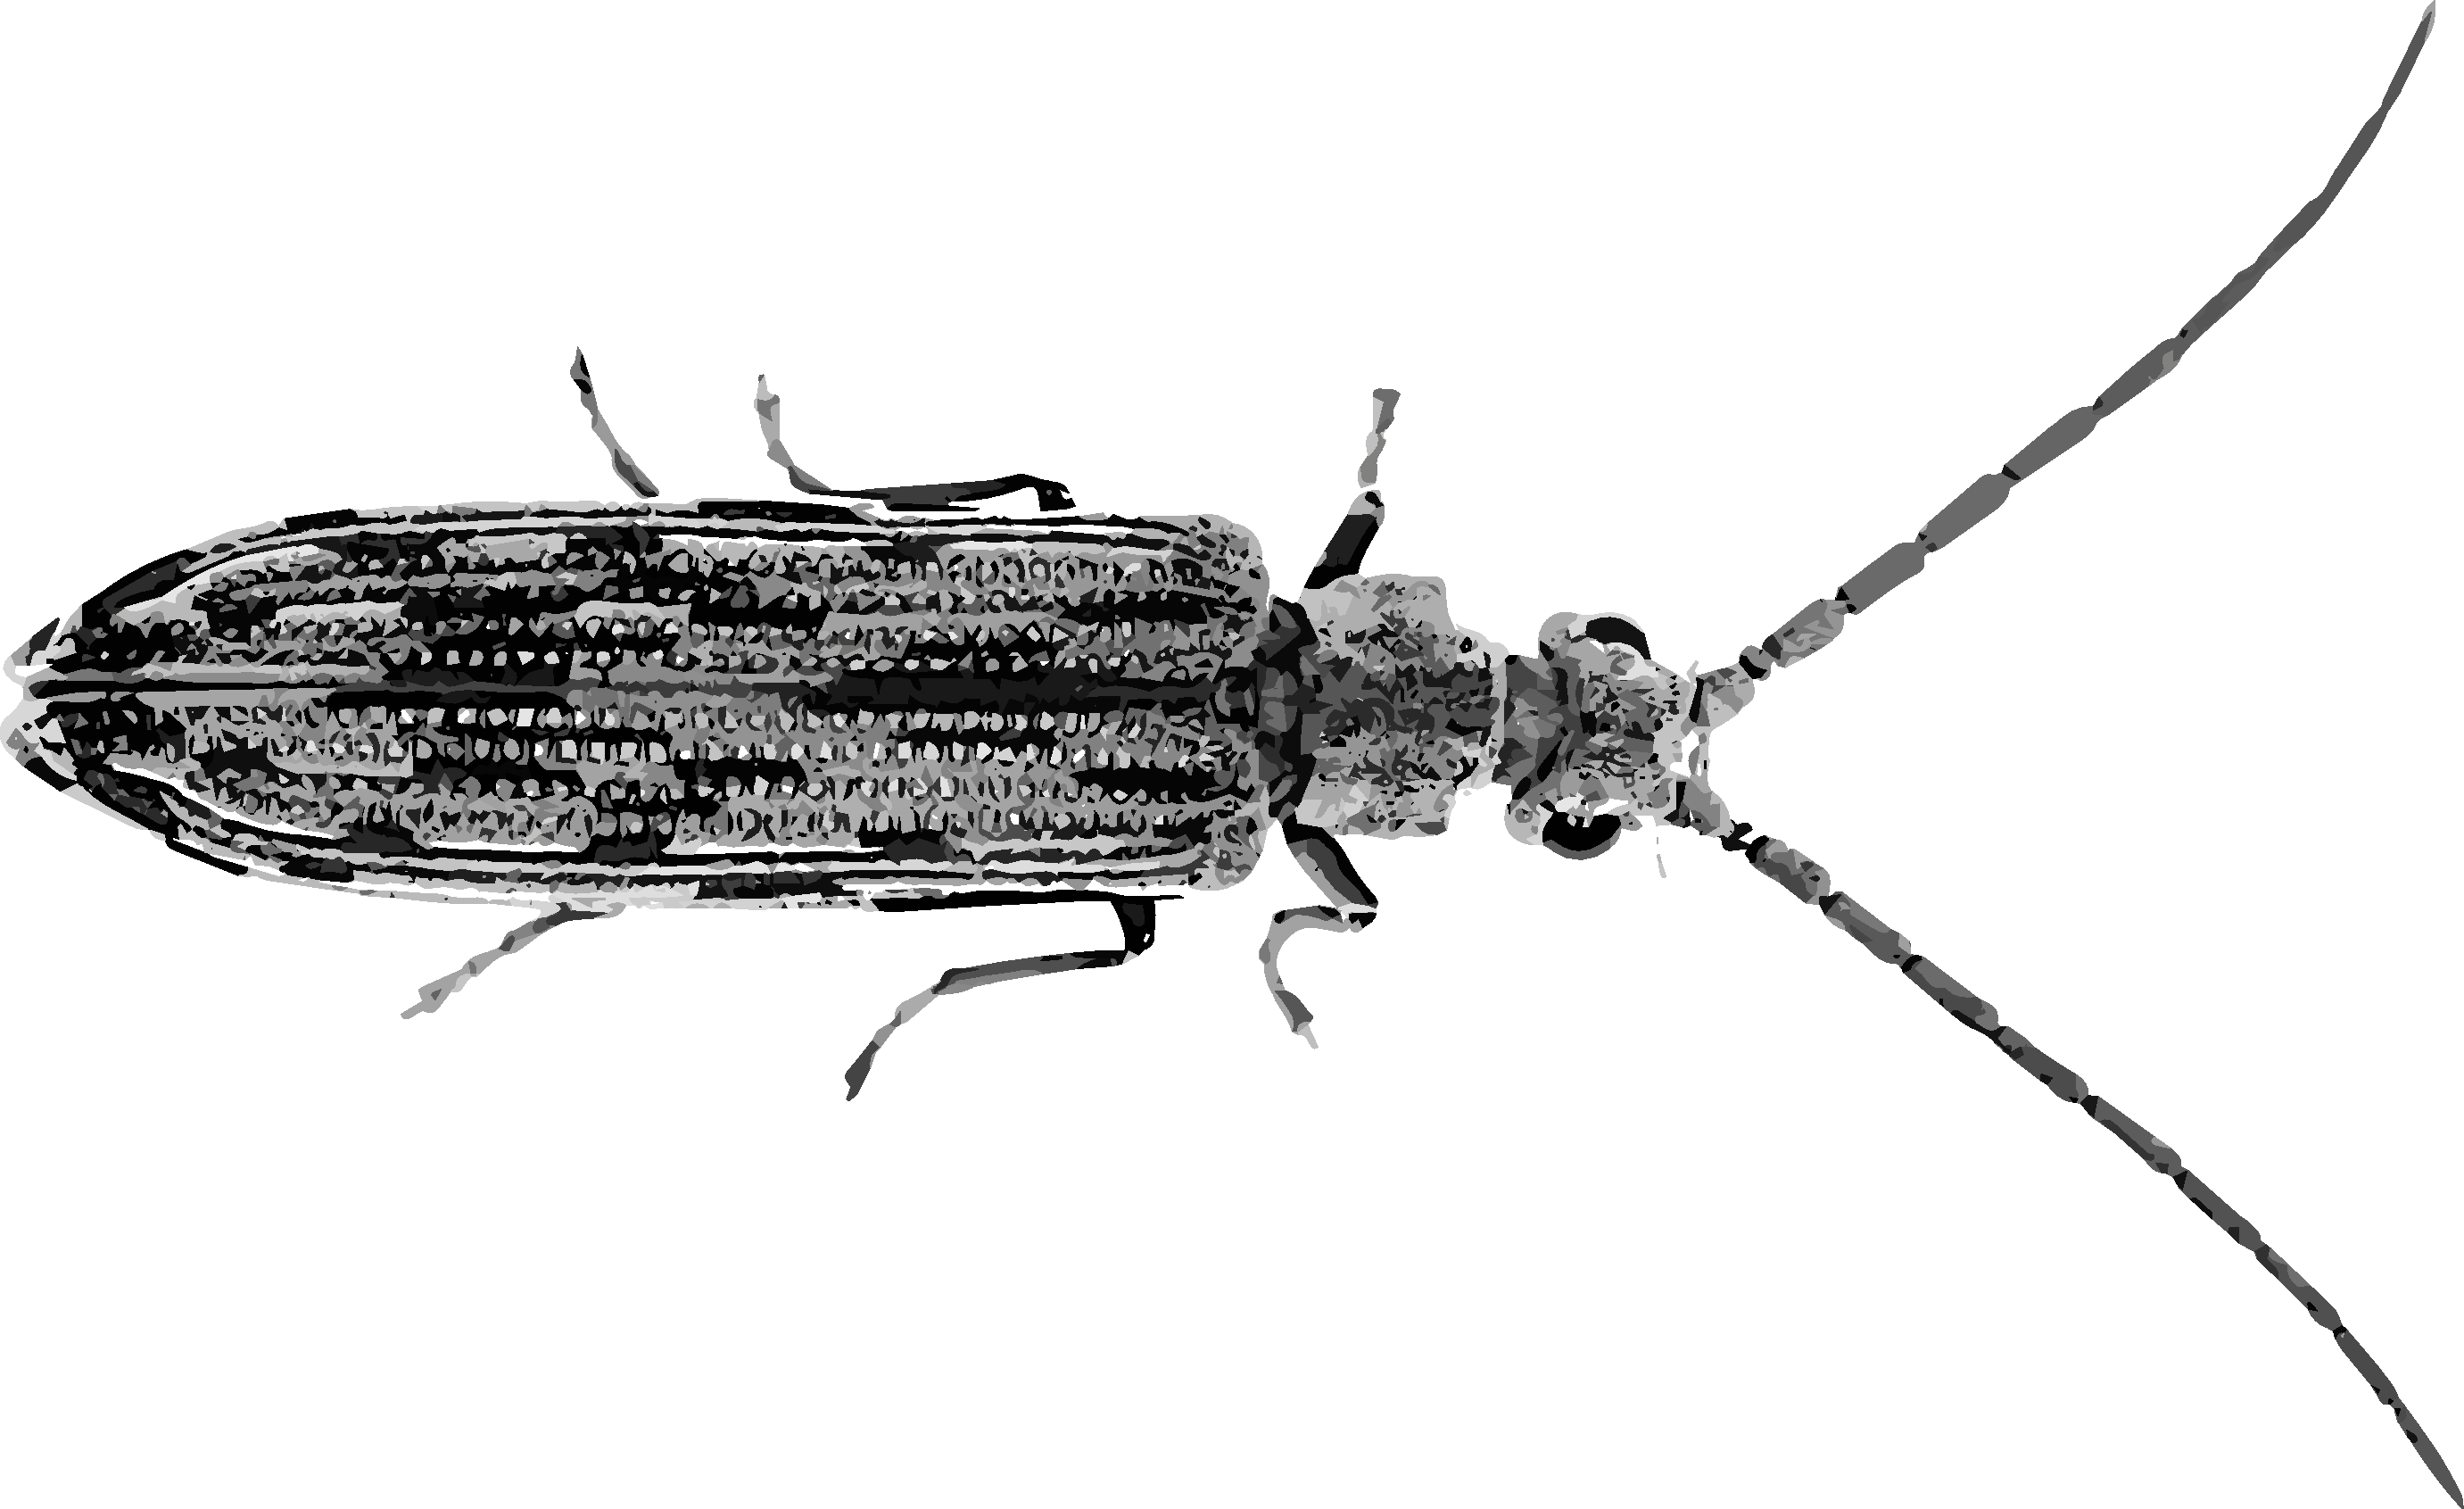
\includegraphics[width=0.6\textwidth]{coleopterida/CupedidHabitus}
  \caption{Cupedidae. Redrawn from photo (CC BY-NC-SA 2.0) by Patrick Coin \url{https://flic.kr/p/5zAYrU}}
  \label{fig:cupedid}%need line drawing or black and white
\end{figure}

\subsection{Adephaga}\index{Adephaga}
\begin{itemize}
\item antenna almost always thread-like
\item notopleural suture present 
\item hind trochanter partially separated from hind femur and coxa %(Figure \ref{fig:adephagaventral}{}, \texorpdfstring{tr\textsubscript{3}}{})
\item hind coxa dividing first abdominal sternite
\end{itemize}
With almost 50,000 known species, this is one of the two largest suborders of beetles. Most species are predaceous, but some feed on algae, seeds, and/or fungi. This taxon is often further divided into Geadephaga (terrestrial families; primarily Carabidae) and Hydradephaga (aquatic species; Gyrinidae, Dytiscidae, Haliplidae, \textit{etc}.) 

\subsubsection{Carabidae (ground beetles)} \index{Carabidae}
\noindent{}\textit{Diagnostic characters:} Antennae threadlike, inserted between eyes and mandibles; fore tibia with antenna cleaner (Can you find it?); legs cursorial.\vspace{3mm}

\noindent{}\textit{Natural history:} Most species are predators of other invertebrates, although there are many that feed on plant material, especially seeds. This family is extraordinarily diverse, with about 40,000 species described.

\begin{figure}[ht!]
  \centering
\begin{subfigure}[ht!]{0.44\textwidth}
   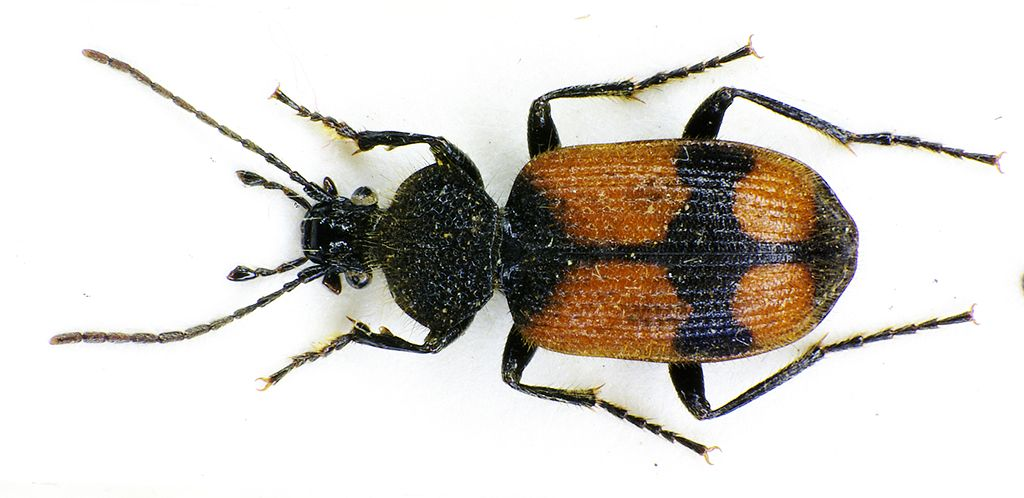
\includegraphics[width=\textwidth]{coleopterida/CarabidHabitus}
   \caption{}
    \label{fig:carab2}
\end{subfigure}
    \qquad
\begin{subfigure}[ht!]{0.48\textwidth}
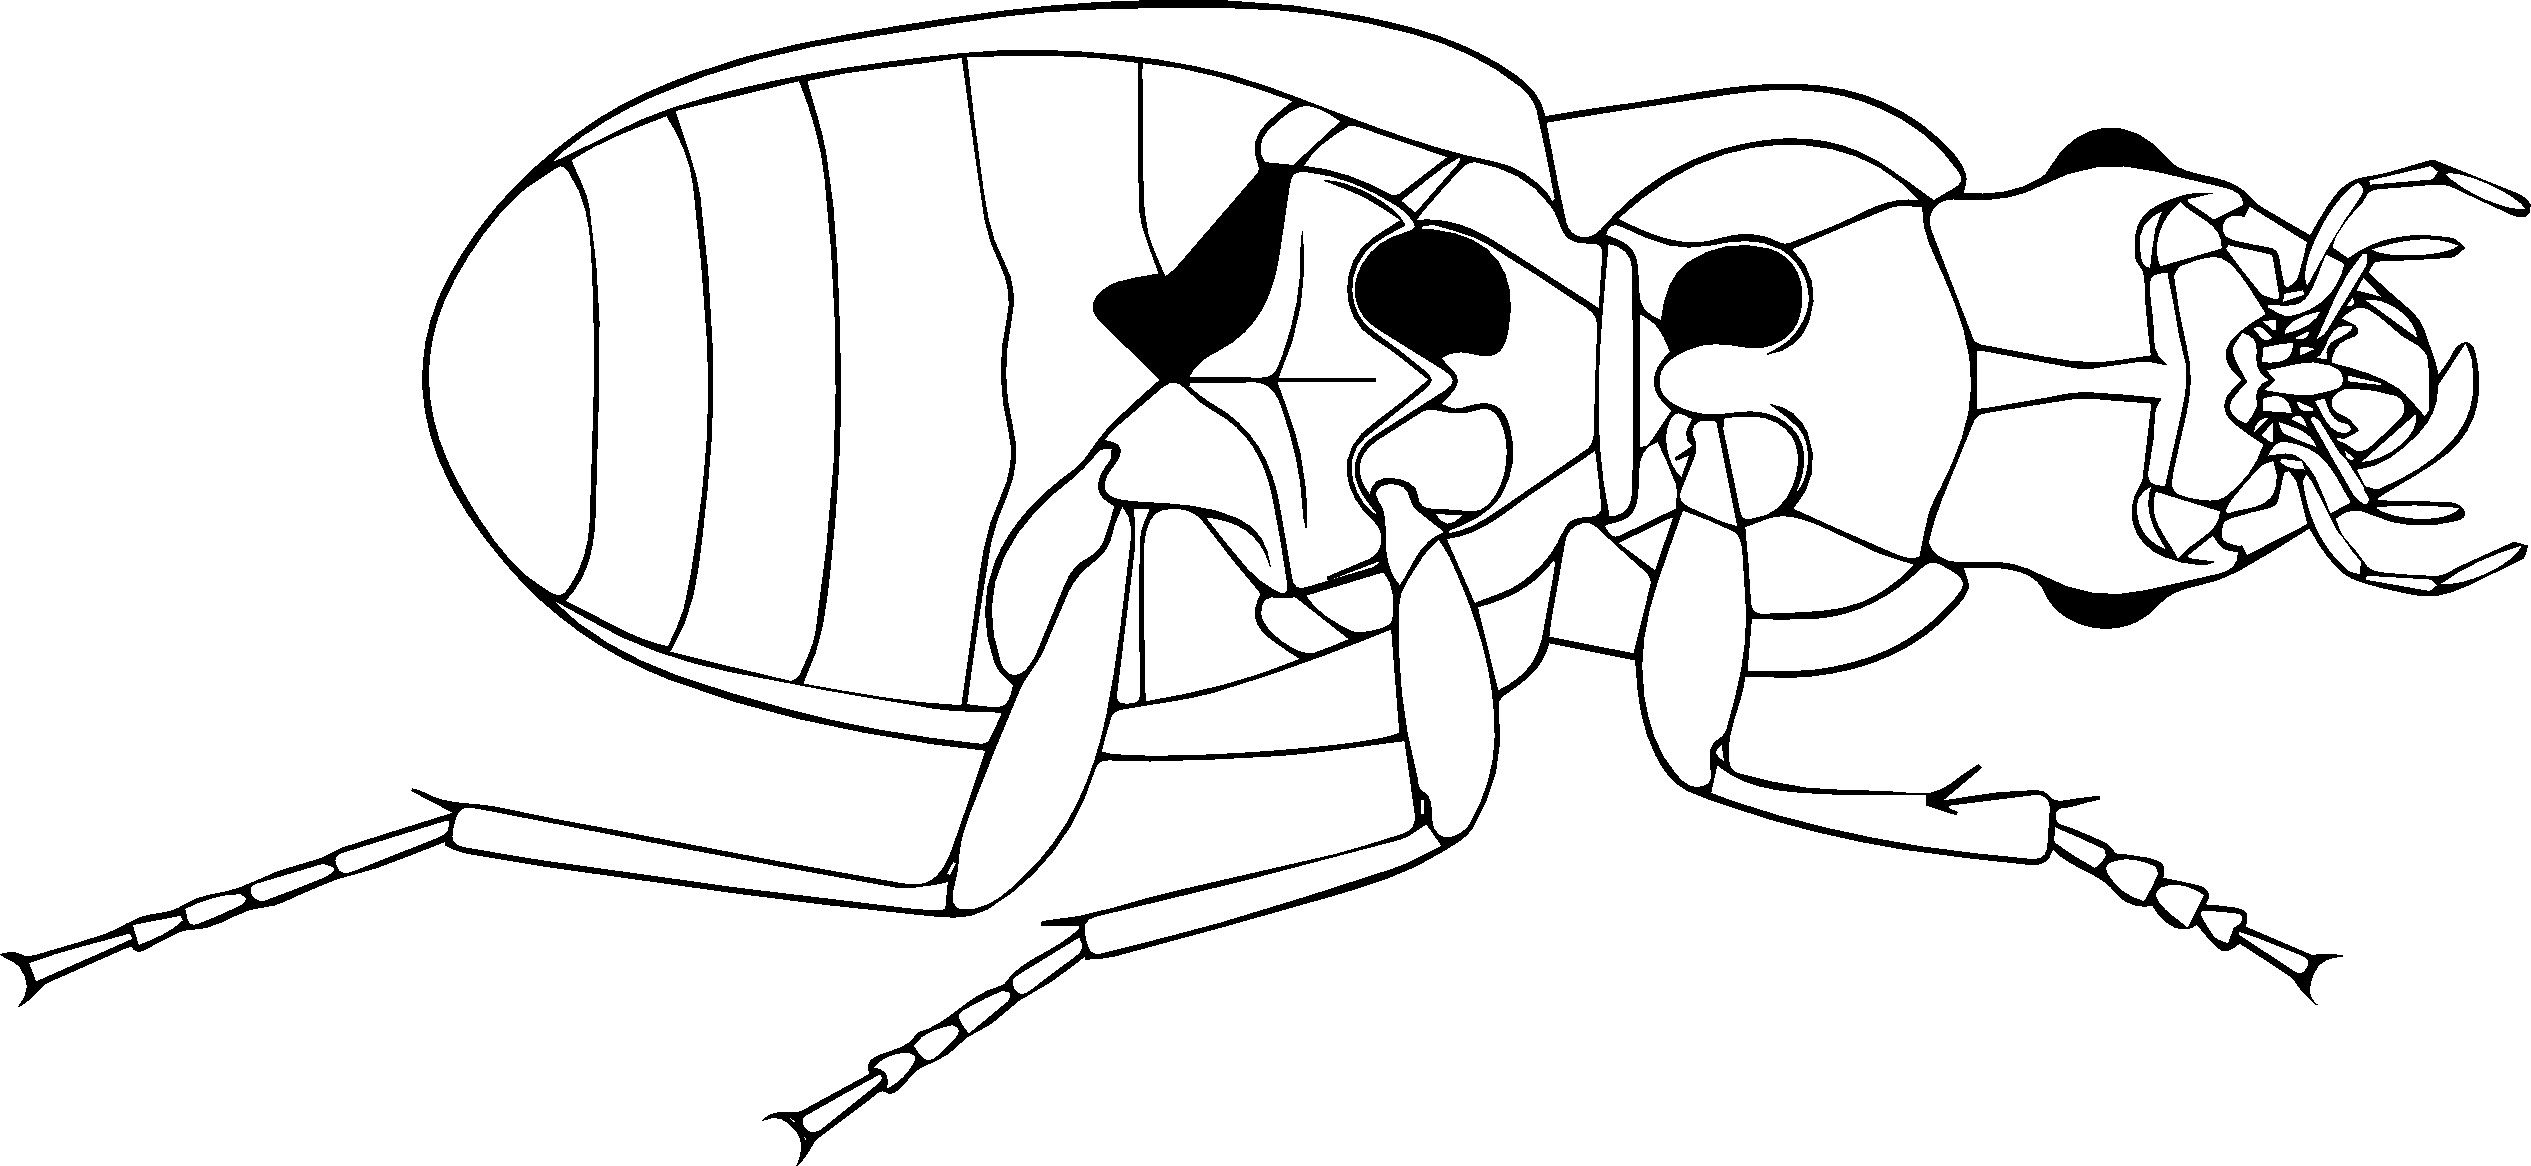
\includegraphics[width=\textwidth]{coleopterida/carabidVentral}
   \caption{}
    \label{fig:carabVentral}
\end{subfigure}
    \caption{Carabidae. (a) Dorsal habitus \citep[Modified from][Plate 24, Fig. 1b]{reitter1908fauna}; (b) ventral habitus (modified from illustration by Des Helmore, Manaaki Whenua – Landcare Research)}
\end{figure}

\subsubsection{Haliplidae (crawling water beetles)}\index{Haliplidae}
\noindent{}\textit{Diagnostic characters:} Body oval, tapered at both ends, convex above, head relatively small; antennae threadlike but fairly short; hind coxae greatly enlarged into flat plates, covering 2 or more abdominal segments (figure \ref{fig:haliplididvent}).\vspace{3mm}

\noindent{}\textit{Natural history:} These beetles are aquatic, and they store air in the expanded region near their hind coxae. Approximately 200 species have been described, all of which feed primarily on algae. They can usually be found crawling around in aquatic vegetation.

\begin{figure}[ht!]
  \centering
\begin{subfigure}[ht!]{0.22\textwidth}
   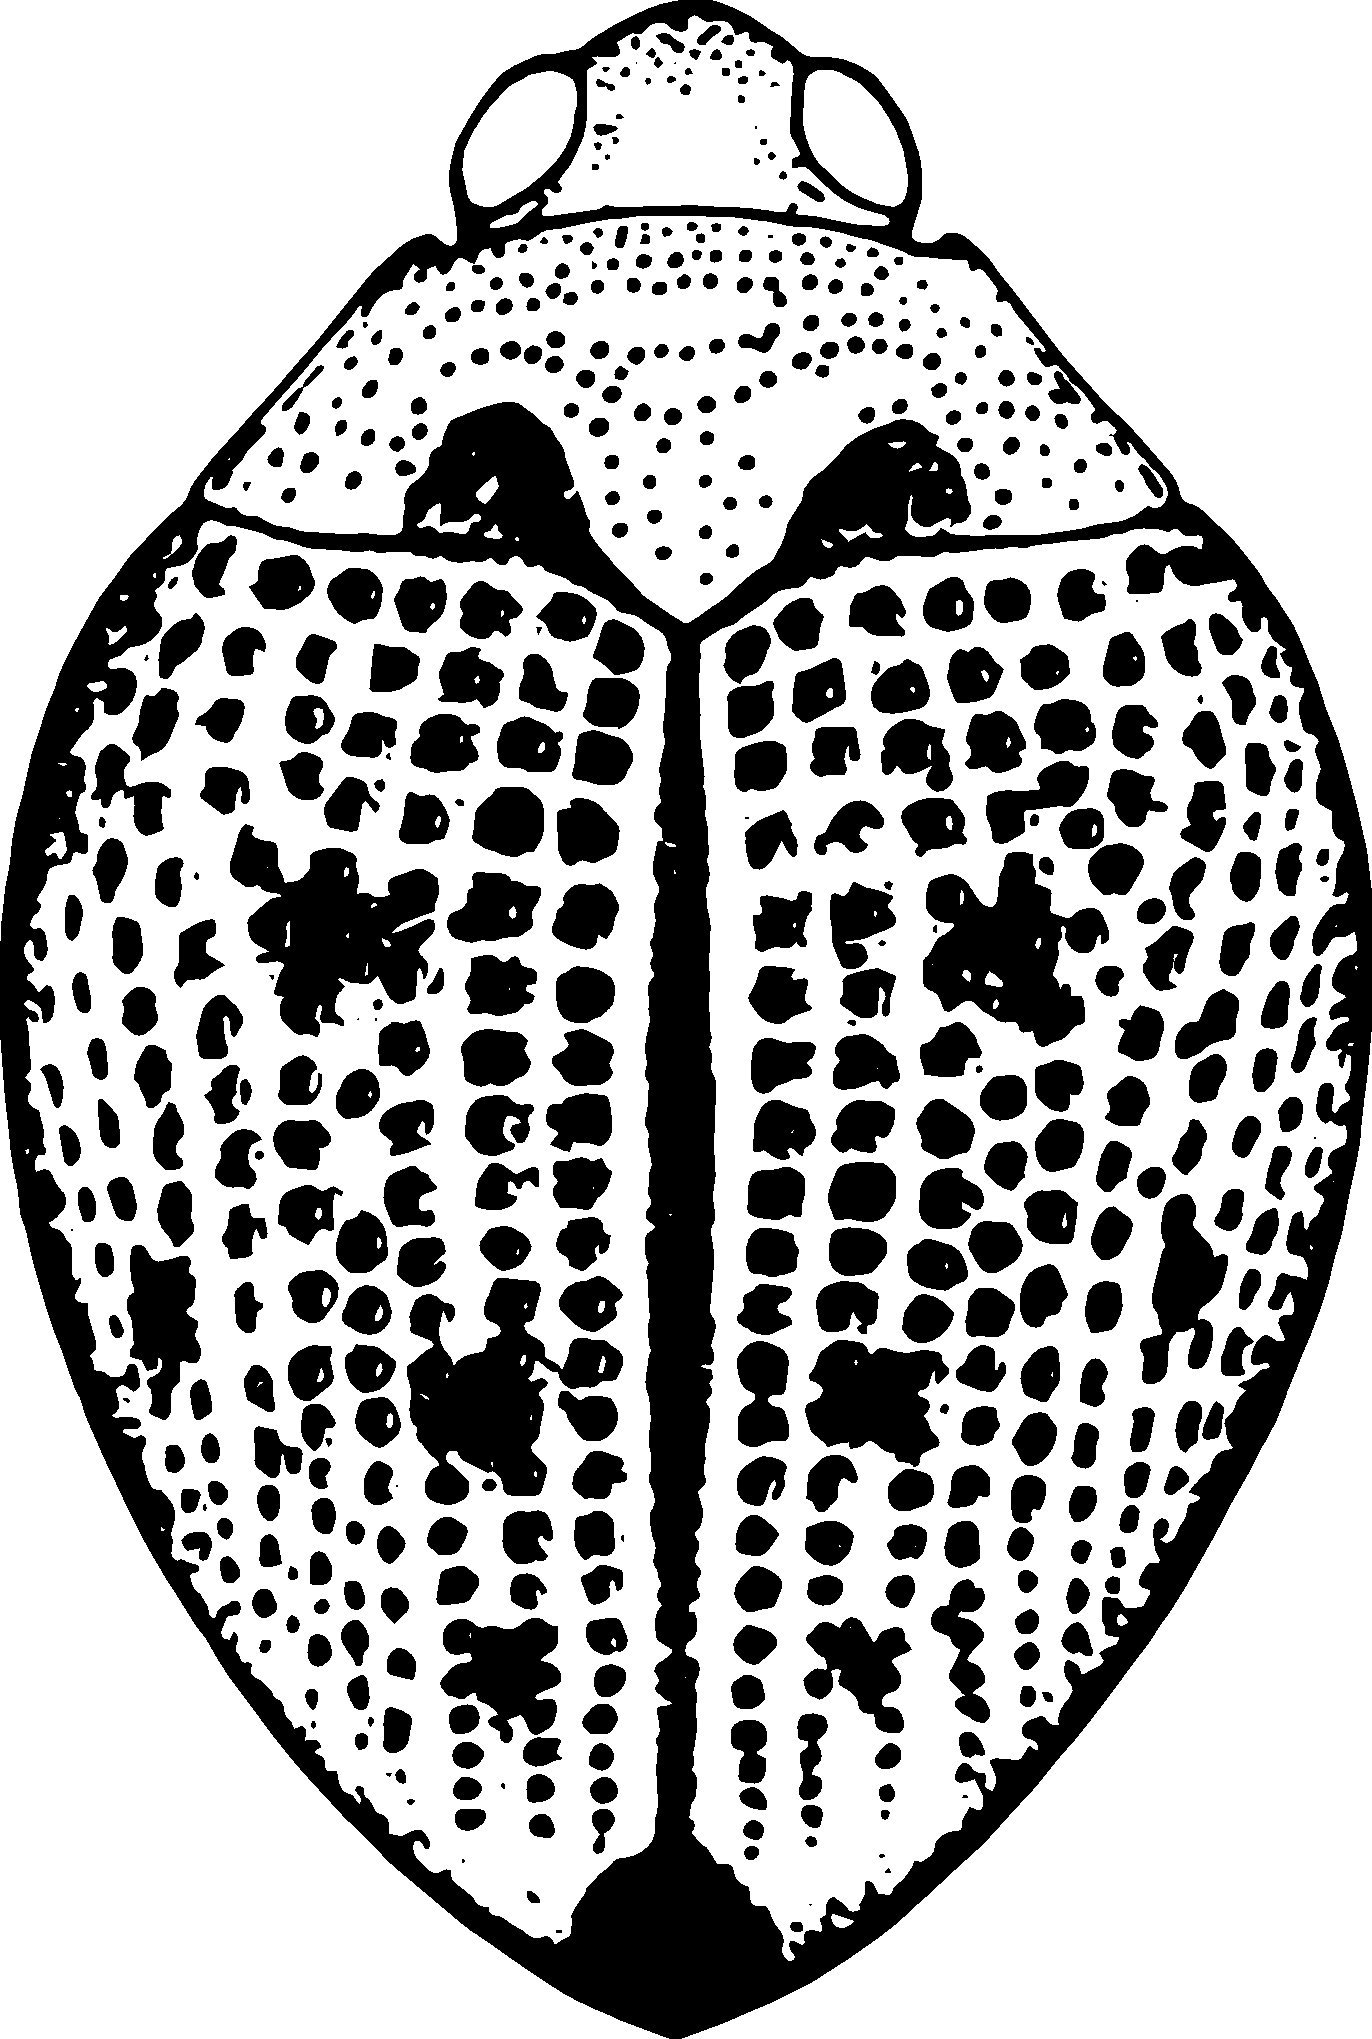
\includegraphics[width=\textwidth]{coleopterida/HaliplidHabitus}
   \caption{}
    \label{fig:halipliddors}
\end{subfigure}
    \qquad
\begin{subfigure}[ht!]{0.45\textwidth}
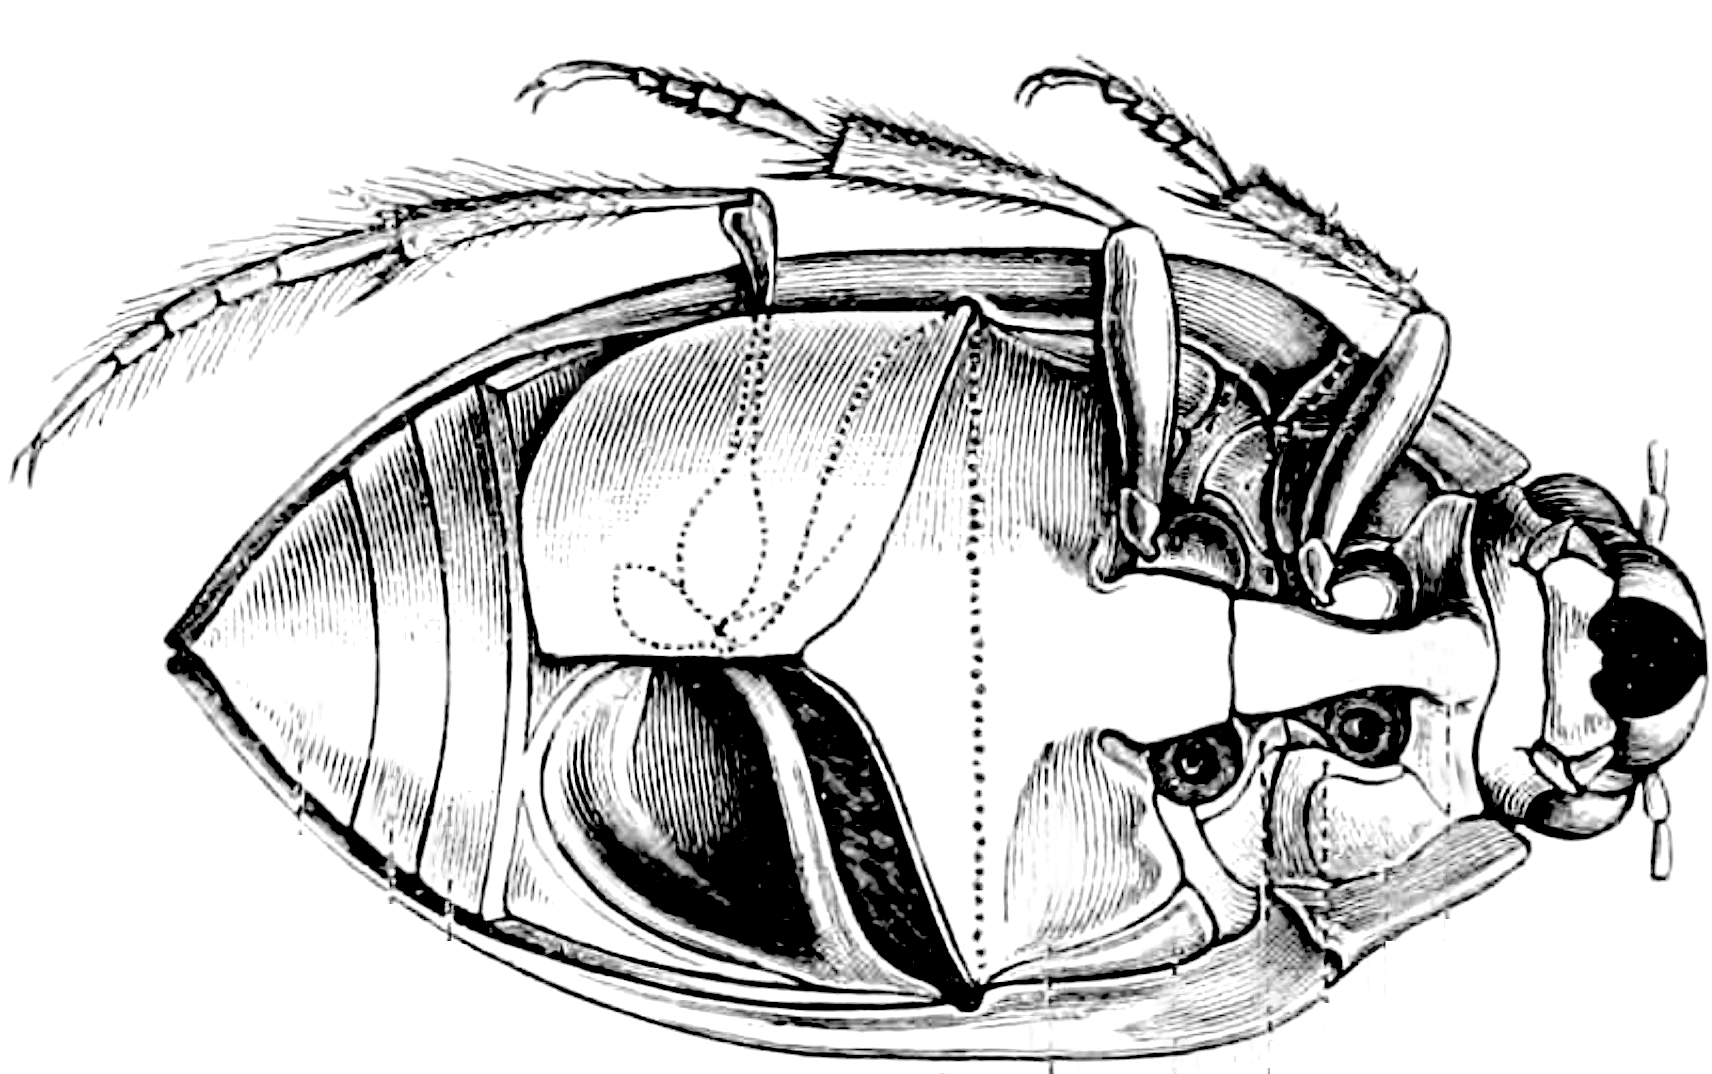
\includegraphics[width=\textwidth]{coleopterida/HaliplidHabitus2}
   \caption{}
    \label{fig:haliplididvent}
\end{subfigure}
    \caption{Haliplidae. (a) Dorsal habitus \citep[][Fig. 13:4a]{bhlitem126080aquatic}; (b) ventral habitus \citep[][Fig. 34]{bhlitem36600}}
\end{figure}


\subsubsection{Gyrinidae (whirligig beetles)}\index{Gyrinidae}
\noindent{}\textit{Diagnostic characters:} Eyes appear to be divided into 2 parts (figure \ref{fig:gyrinidhead}); fore legs long, other legs short and flat like paddles; pedicel relatively large (Johnston's organ used to detect prey); antenna clubbed; body elongate-oval, dorso-ventrally flattened.\vspace{3mm}

\noindent{}\textit{Natural history:} These beetles are semi-aquatic and are usually found skimming across the surface in large aggregations. Approximately 700 species have been described worldwide.

\begin{figure}[ht!]
  \centering
    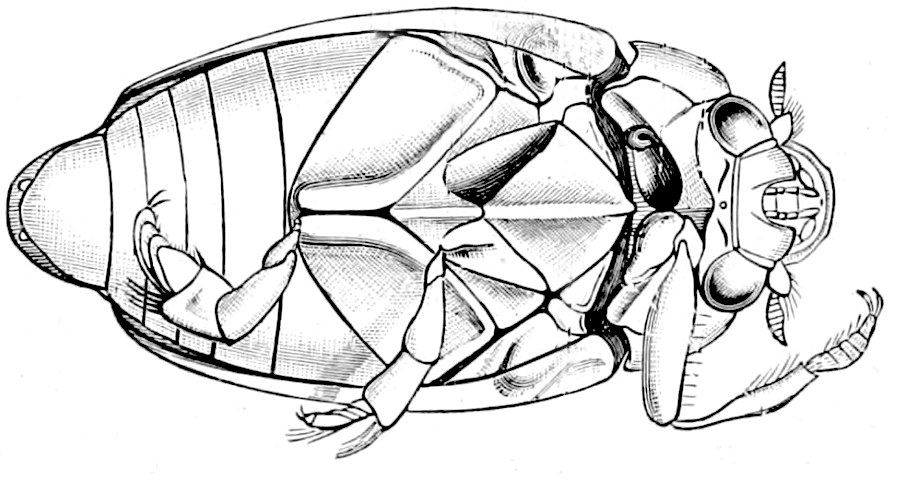
\includegraphics[width=0.5\textwidth]{coleopterida/gyrinid}
  \caption{Gyrinidae ventral habitus \citep[][Fig. 99B]{bhlitem56570}}
  \label{fig:gyrnidhabitus}
\end{figure}

\begin{figure}[ht!]
  \centering
\begin{subfigure}[ht!]{0.3\textwidth}
    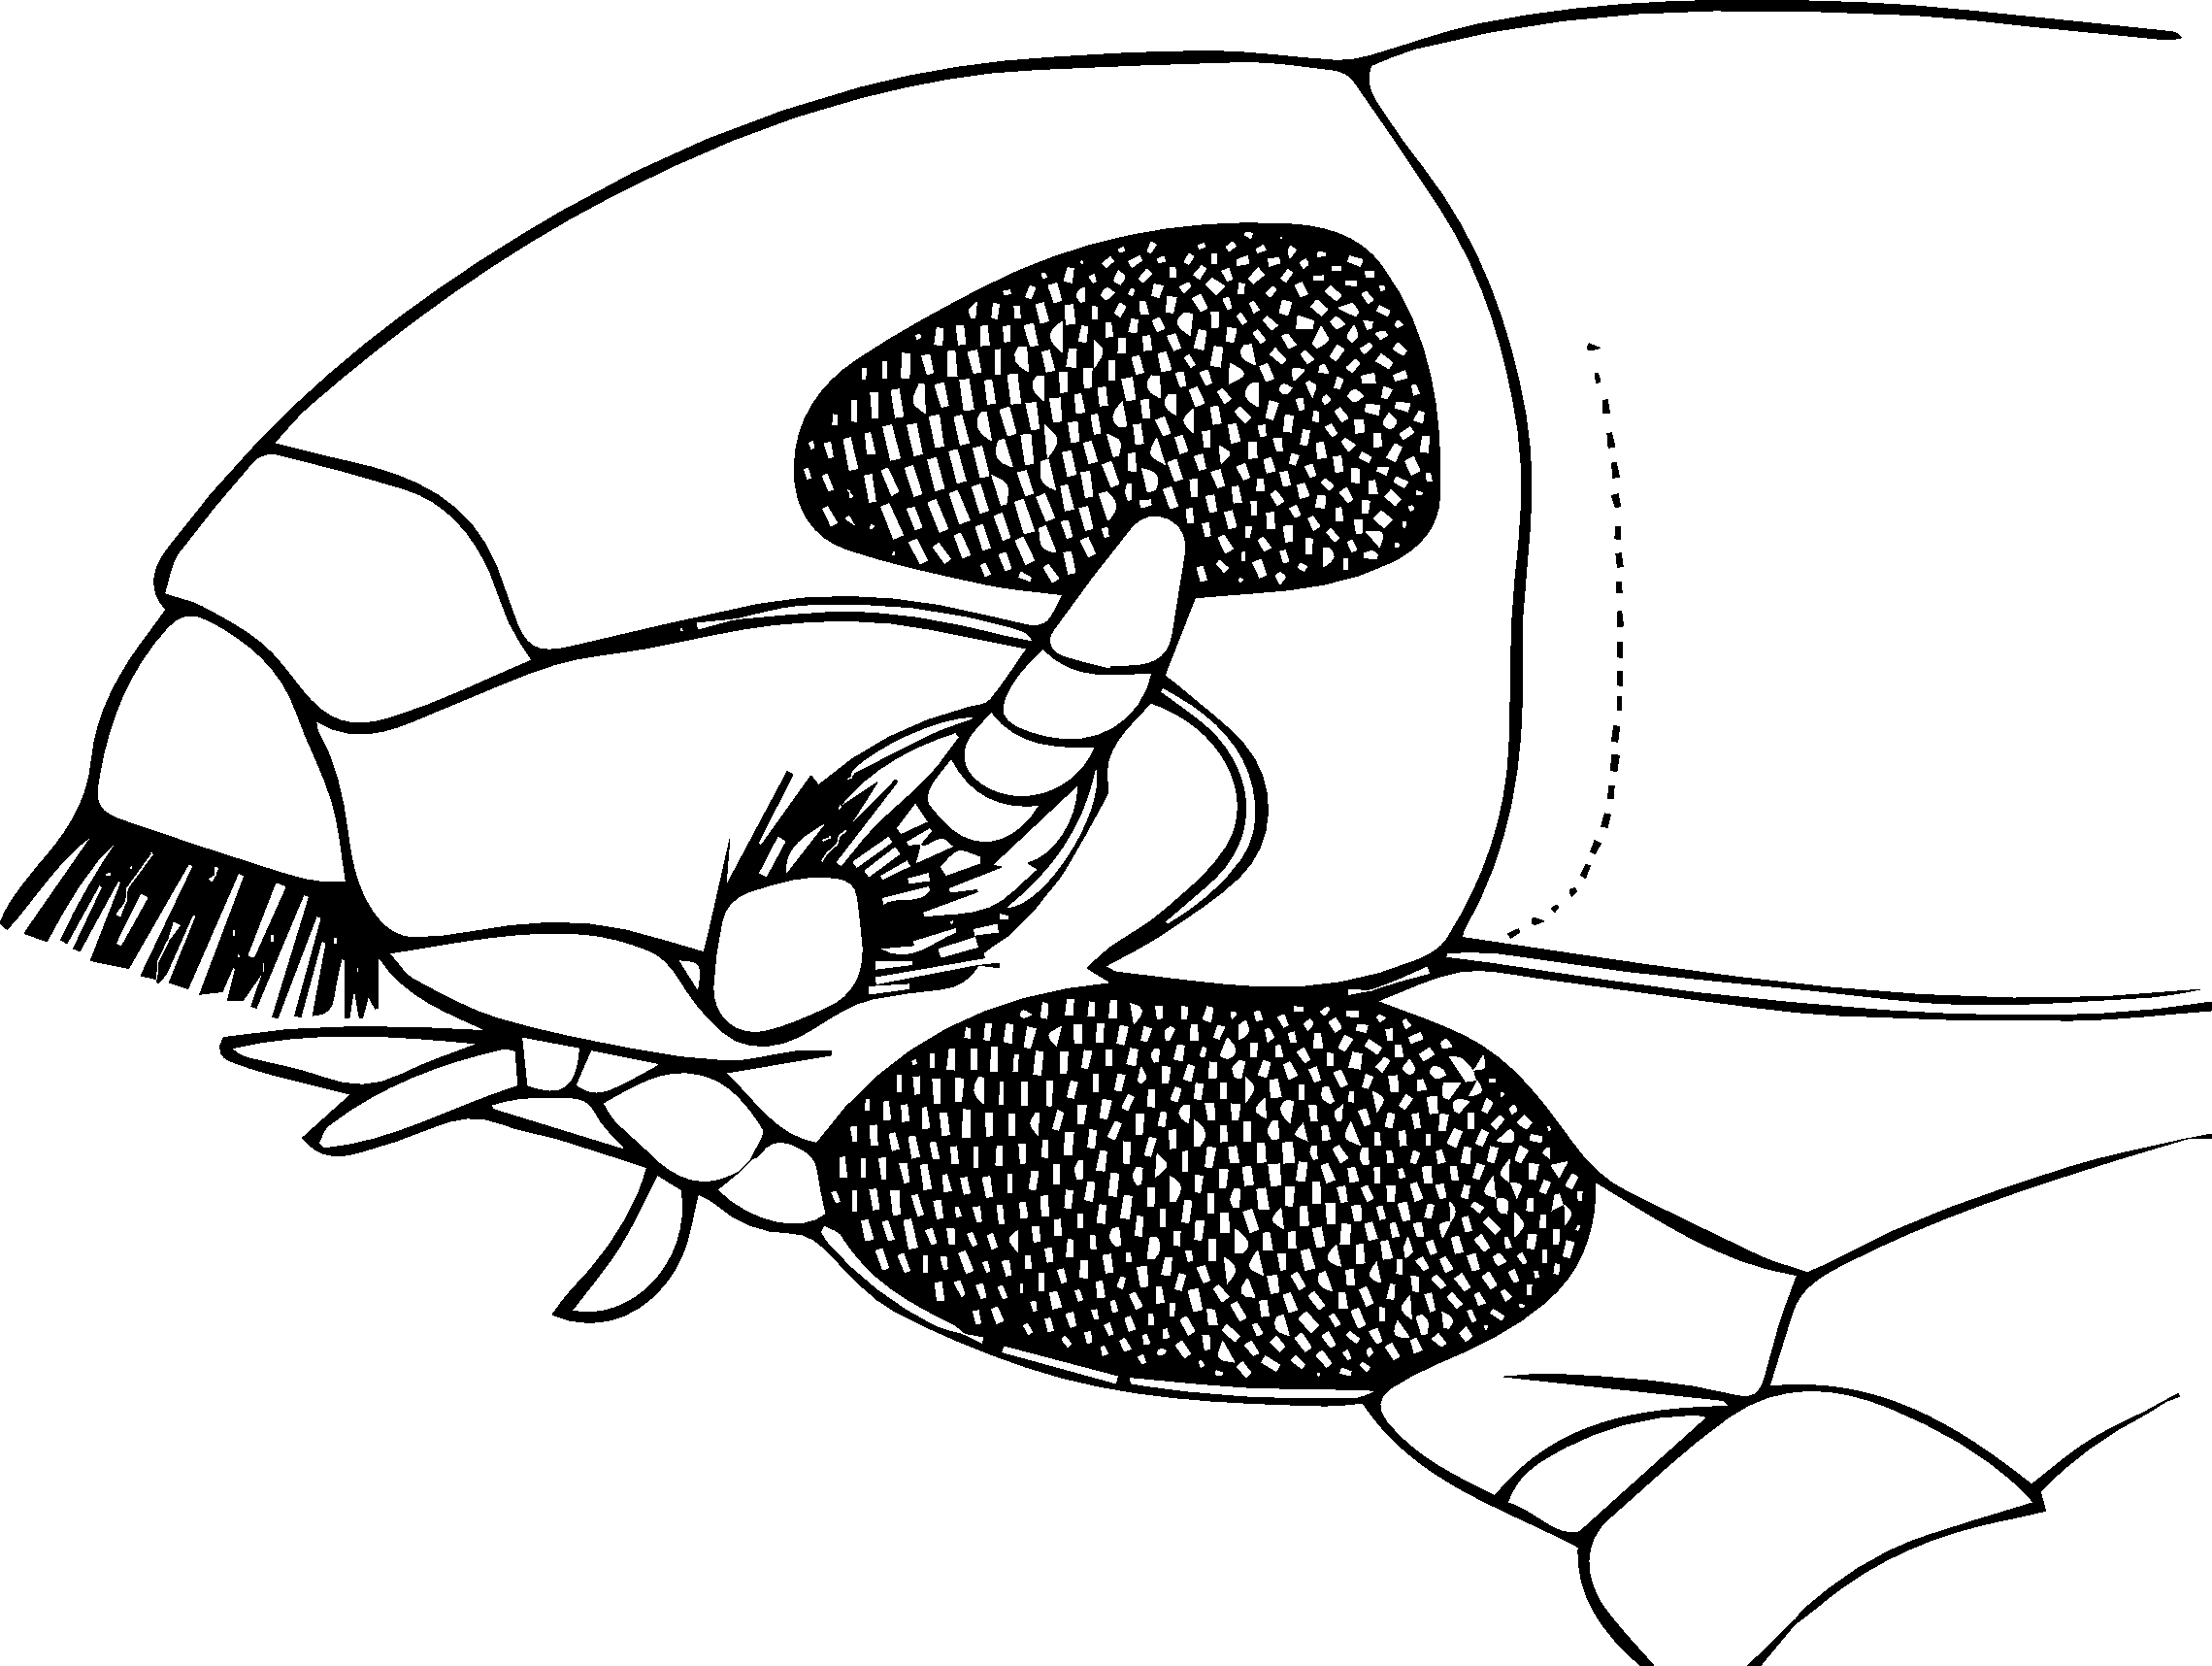
\includegraphics[width=\textwidth]{coleopterida/gyrinidHead}
  \caption{}
  \label{fig:gyrinidhead}
\end{subfigure}
    \hfill
\begin{subfigure}[ht!]{0.3\textwidth}
    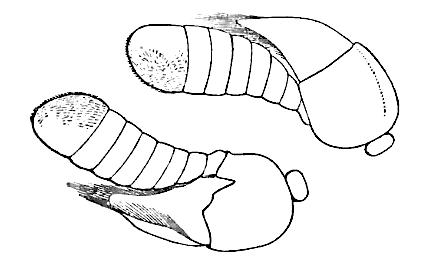
\includegraphics[width=\textwidth]{coleopterida/GyrinidAntennae}
  \caption{}
  \label{fig:gyrinidantenna}
\end{subfigure}
    \caption{Gyrinidae. \textbf{(a)} Head \citep[][Fig. 13:23]{bhlitem126080aquatic}; \textbf{(b)} antennae, illustration by Stavely (1873)}\label{fig:gyrinids}
\end{figure}

\subsubsection{Dytiscidae (predaceous diving beetles)}\index{Dytiscidae}
\noindent{}\textit{Diagnostic characters:} Body elongate-oval, convex and streamlined; fore tarsi sometimes pseudotetramerous; male tarsi often highly modified for mating (attachment device); hind legs flattened and fringed with hairs for swimming; antennae threadlike, fairly long, longer than palpi.\vspace{3mm}

\noindent{}\textit{Natural history:} These aquatic beetles feed on other invertebrates. They store air under their elytra and swim with both hind legs kicking simultaneously. Approximately 4,000 species have been described worldwide.\vspace{3mm}

\begin{theo}
{}How do the attachment structures work for males? Do you see corresponding structures (or ``defenses'') in females?
\end{theo}

\begin{figure}[ht!]
  \centering
\begin{subfigure}[ht!]{0.4\textwidth}
    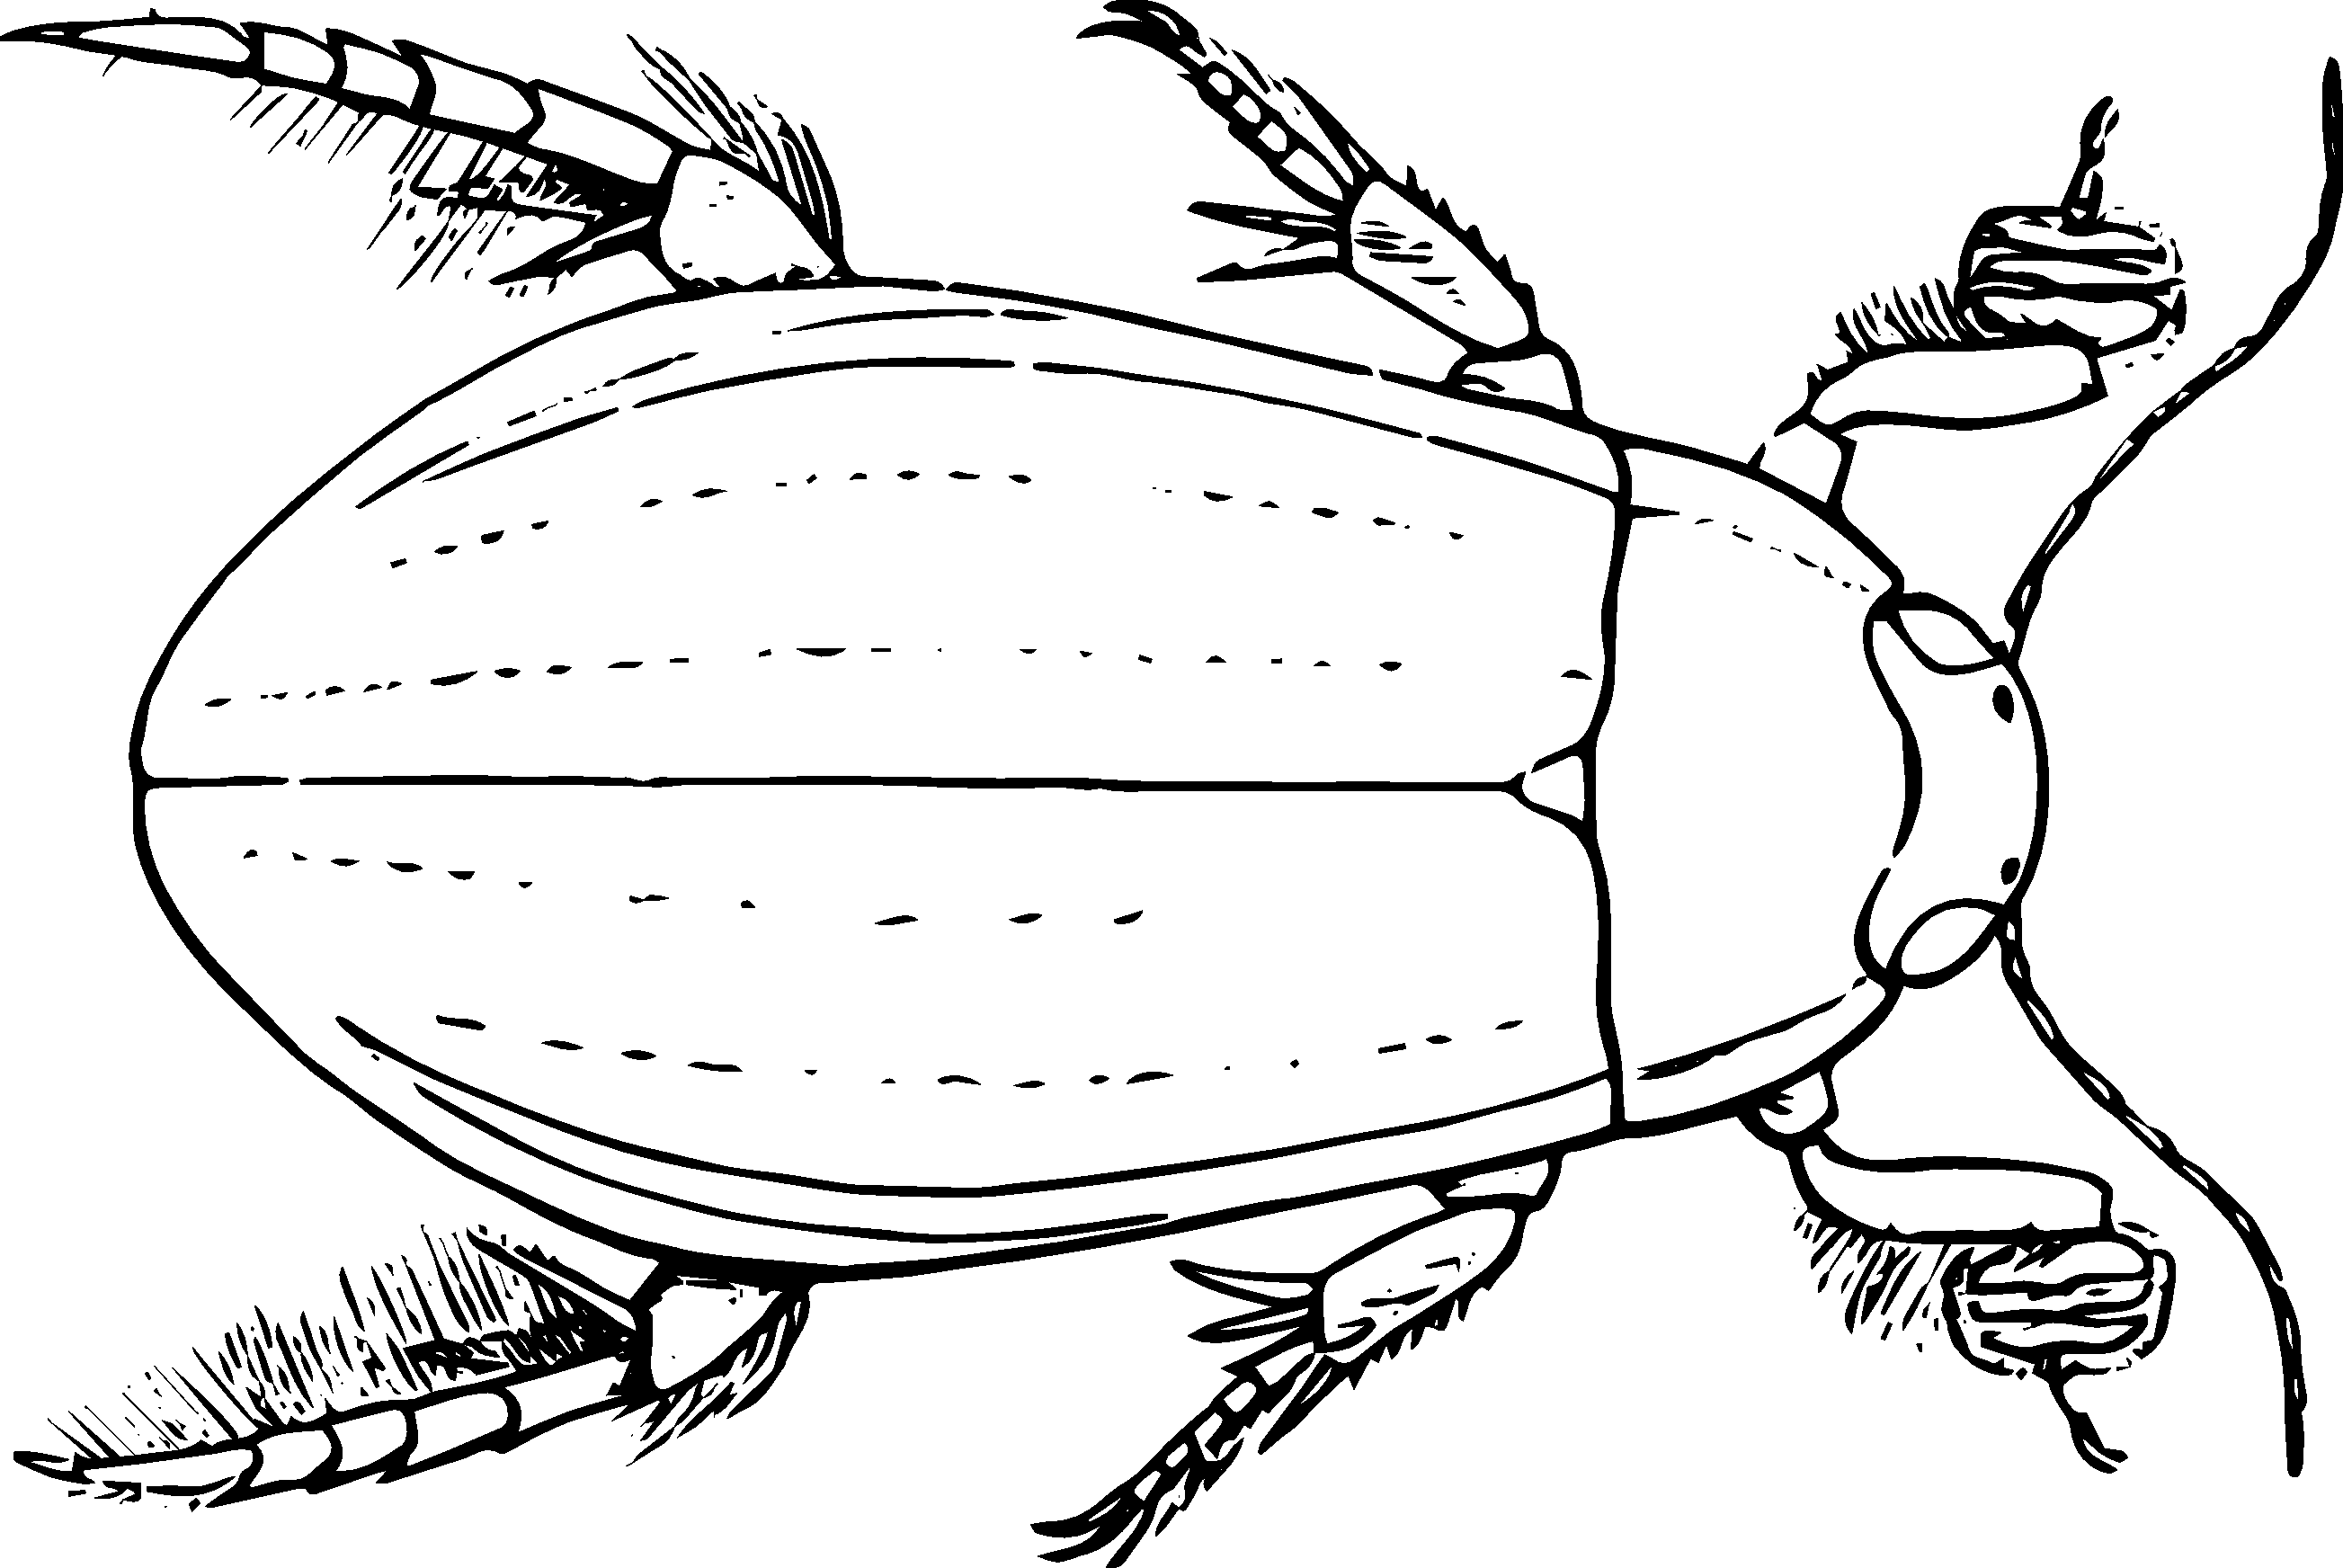
\includegraphics[width=\textwidth]{coleopterida/dyticiddorsal}
  \caption{}
  \label{fig:dytiscidHabitus1}
\end{subfigure}
    \hfill
\begin{subfigure}[ht!]{0.45\textwidth}
    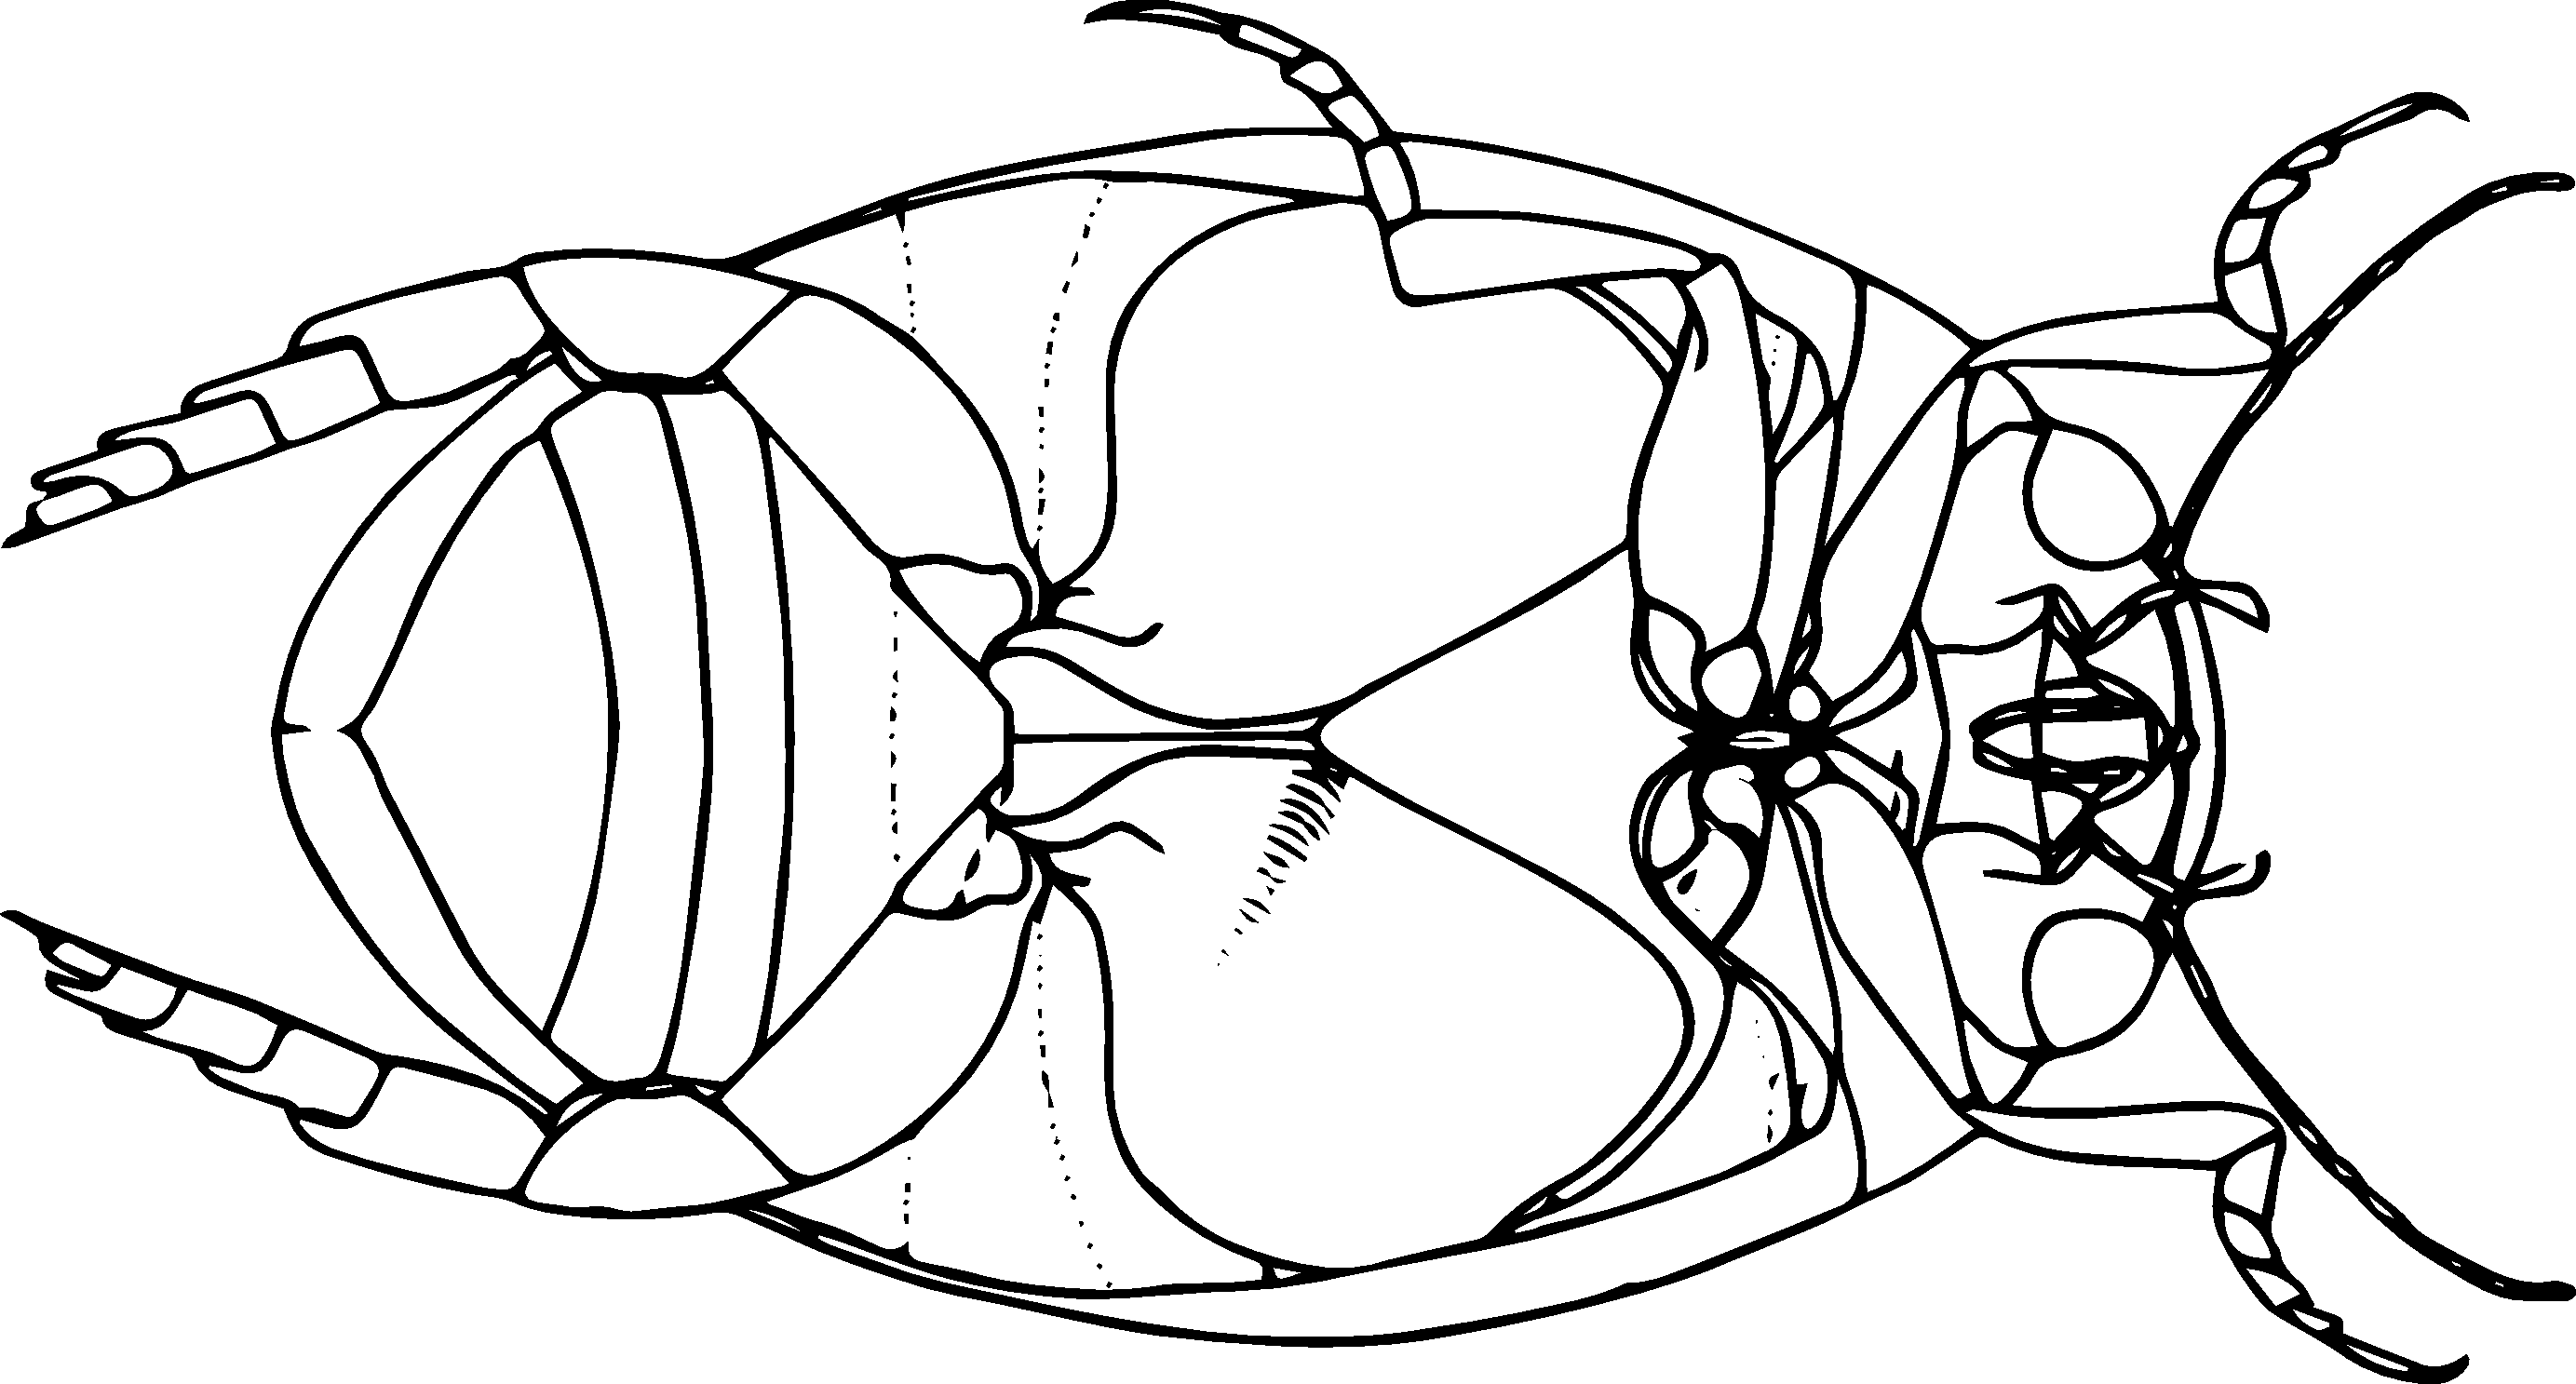
\includegraphics[width=\textwidth]{coleopterida/dytiscidVentral}
  \caption{}
  \label{fig:dytiscidHabitus2}
\end{subfigure}
    \caption{Dytiscidae. \textbf{(a)} Dorsal habitus \citep[][Fig. 96B]{bhlitem56570}; \textbf{(b)} ventral habitus \citep[Modified from Fig. 13:9 in][]{bhlitem126080aquatic}}\label{fig:dytiscids}
\end{figure}

\subsection{Myxophaga}\index{Myxophaga}
This another tiny suborder, with only 65+ species of small to minute beetles that are aquatic or semiaquatic, and feed on algae. These species do not occur in the northeastern USA.

\subsection{Polyphaga}\index{Polyphaga}
\begin{itemize}
\item notopleural suture usually absent
\item hind trochanter not separated and lobe-like (\textit{i.e.}, similar to most other insects) 
\end{itemize}
This lineage is by far the most diverse of the four coleopteran suborders, with \textgreater300,000 described species. These beetles vary considerably in their sizes, morphology, diets, and other life history traits.

\subsubsection{Ptiliidae (feather-wing beetles)}\index{Ptiliidae}
\noindent{}\textit{Diagnostic characters:} Extremely tiny (usually \textless1.2 mm); flight wings feather-like, often partially visible beyond elytra; antennae long, with 2--3-segmented loose club with whorl of setae; pronotum relatively large.\vspace{3mm}

\noindent{}\textit{Natural history:} Approximately 600 species of these minute (0.3--0.5 mm long) beetles have been described, many of which can be easily collected in leaf litter. Their common name is derived from their distinctive hind wing phenotype. These beetles have been the subject of research on the effects of miniaturization.

\begin{figure}[ht!]
  \centering
    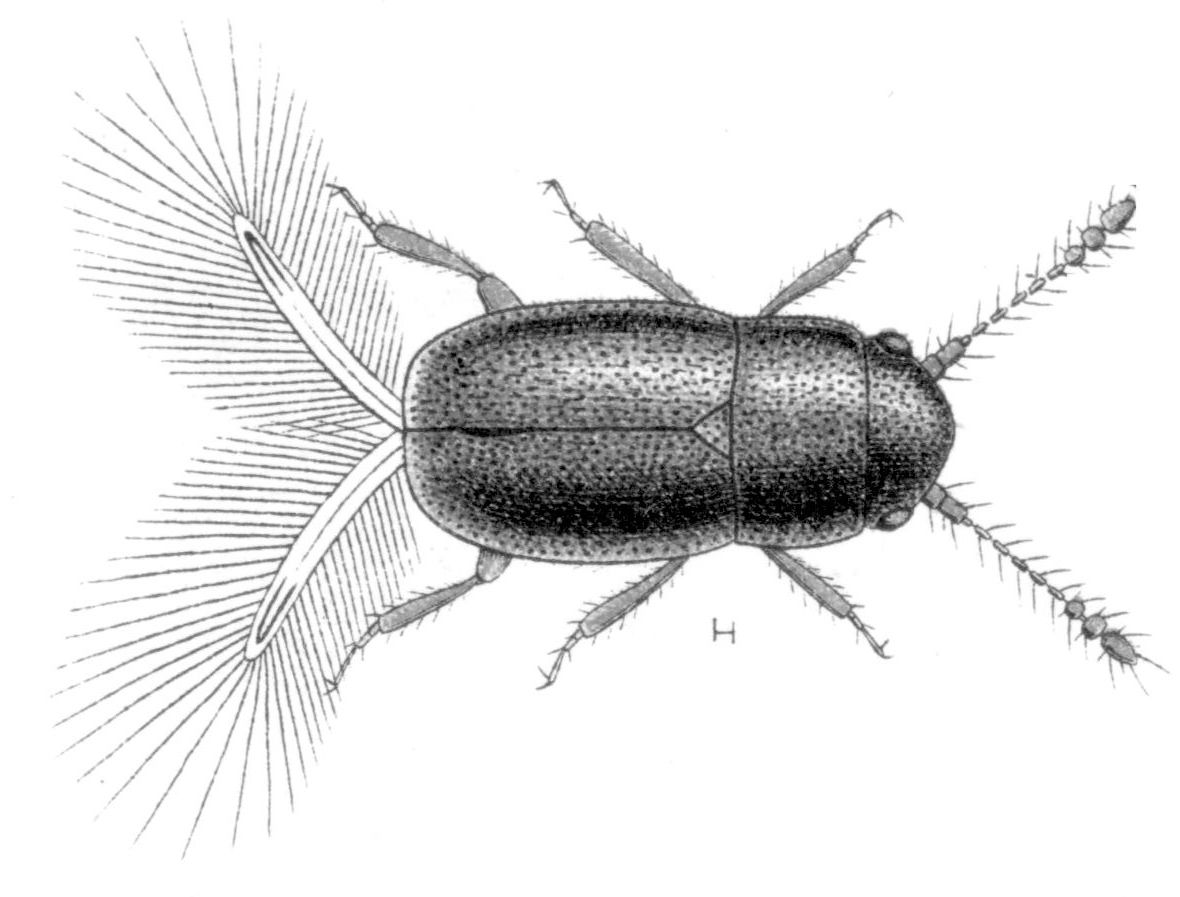
\includegraphics[width=0.5\textwidth]{coleopterida/PtiliidHabitus2}
  \caption{Ptiliidae habitus \citep[Modified from Fig. 17 in][]{reitter1908fauna}}
  \label{fig:ptiliids}
\end{figure}

\subsubsection{Silphidae (carrion beetles)}\index{Silphidae}
\noindent{}\textit{Diagnostic characters:} Elytra broader posteriorly, loosely fitting and not heavily sclerotized; 1 or 2 abdominal tergites exposed posteriorly; antennae with 4-merous asymmetrical club; usually black and orange or yellow, \textgreater12 mm.\vspace{3mm}

\noindent{}\textit{Natural history:} As their common name suggests, these beetles usually process carrion (dead vertebrates, usually, which they bury) for their young. Nearly 200 species have been described worldwide.

\begin{figure}[ht!]
  \centering
    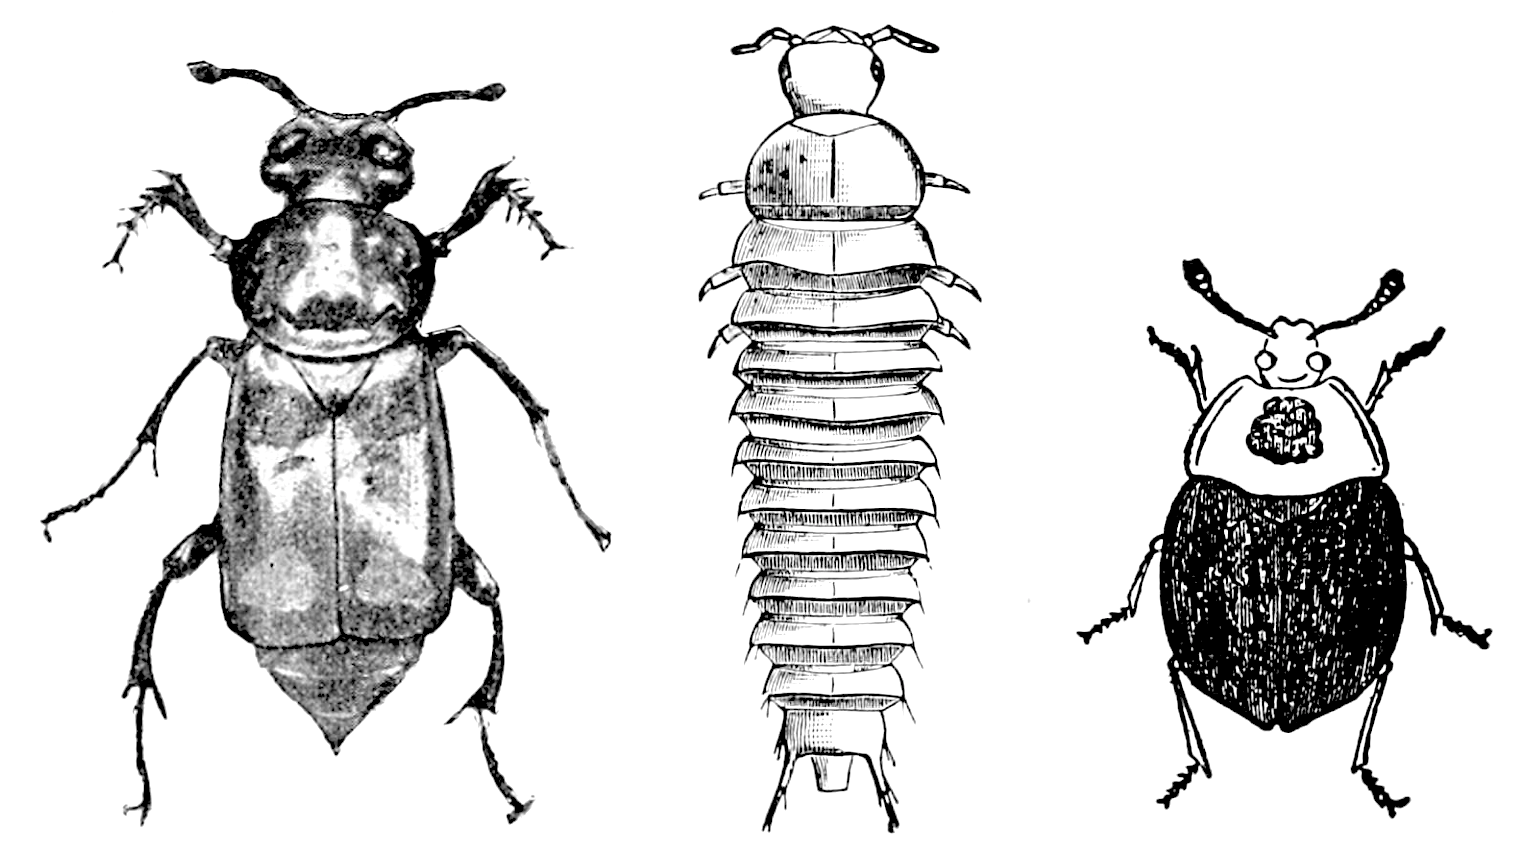
\includegraphics[width=0.5\textwidth]{coleopterida/silphids}
  \caption{Silphidae dorsal habitus \citep[][Fig. 142]{bhlitem92397}}
  \label{fig:silphid}
\end{figure}

\subsubsection{Staphylinidae (rove beetles)}\index{Staphylinidae}
\noindent{}\textit{Diagnostic characters:} Body usually elongate, slender; antennae usually thread-like; elytra almost always short, exposing 3--6 (usually 5--6) abdominal segments.\vspace{3mm}

\noindent{}\textit{Natural history:} This family is \textit{extraordinarily} diverse, with \textgreater60,000(!) described species, and therefore it is difficult to find a consistent set of easy-to-see diagnostic characters. Predation is the most common life history. Many species are saprophages, however,and even a few are parasitoids (of dipteran puparia).\vspace{3mm}

\begin{theo}
{}Why do staphylinids have short elytra? Think about where they live. What are the consequences of having such short elytra?
\end{theo}

\begin{figure}[ht!]
  \centering
    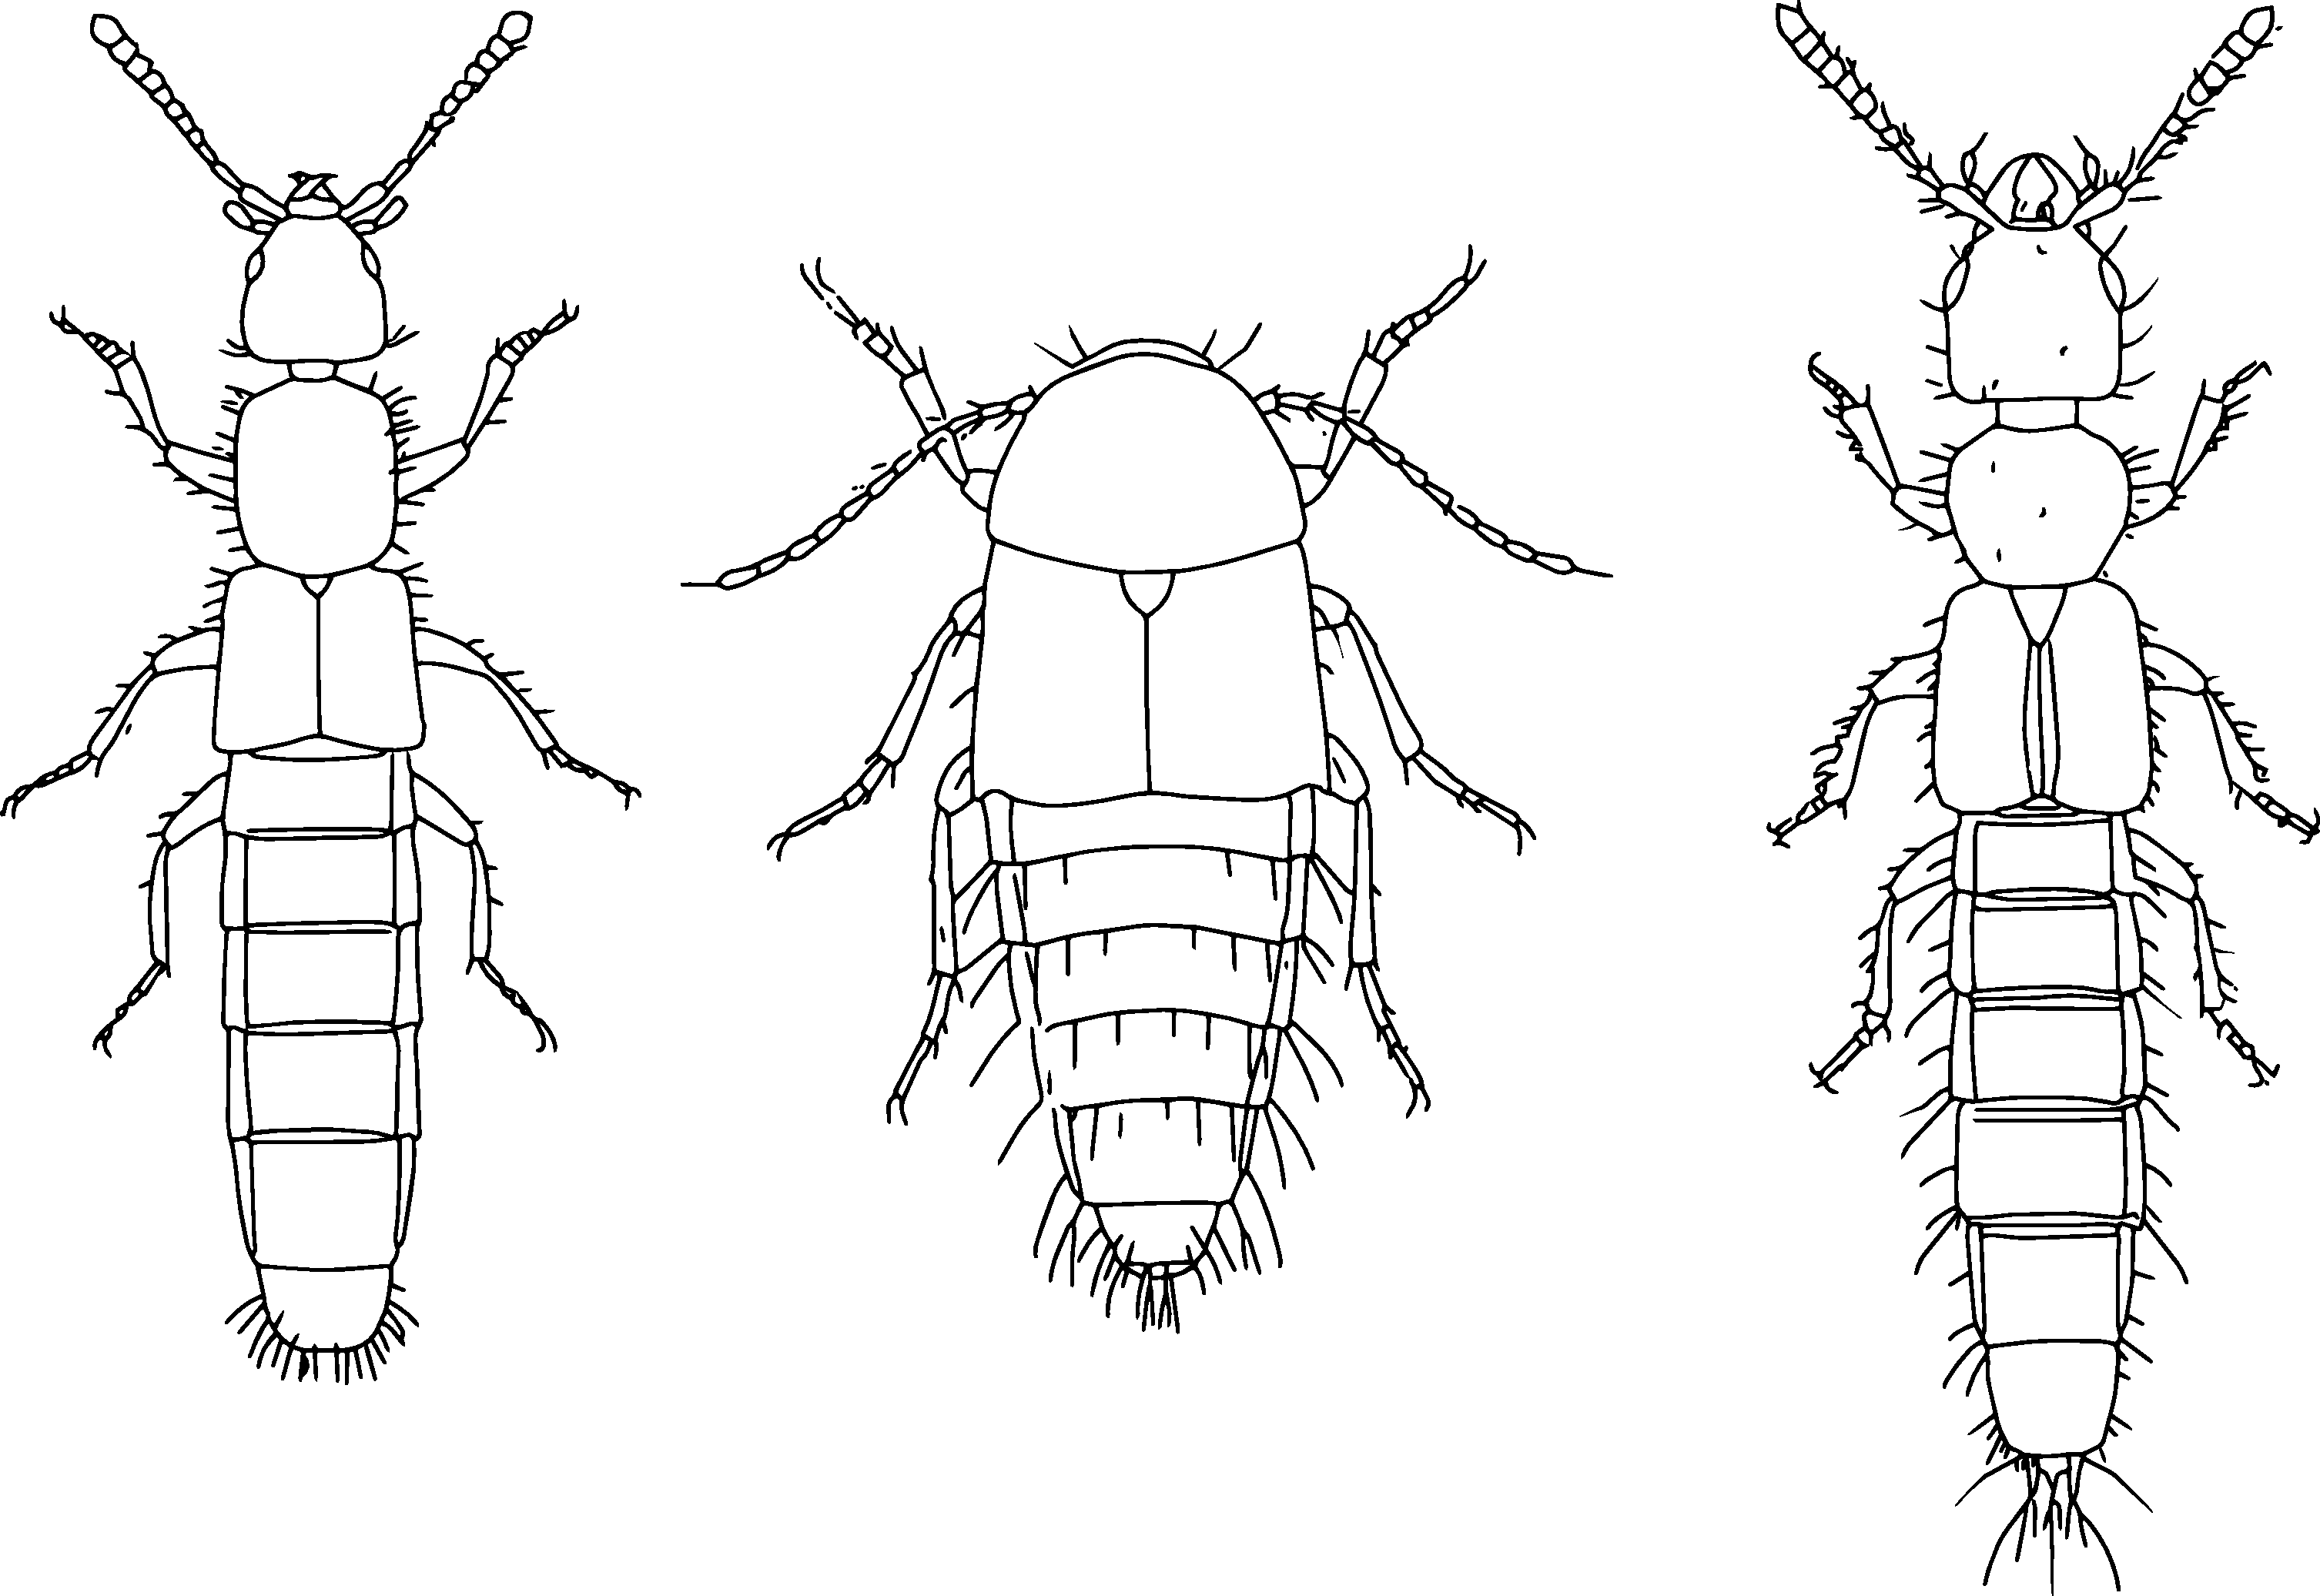
\includegraphics[width=0.65\textwidth]{coleopterida/staphylinids}
  \caption{Staphylinidae dorsal habitus \citep[][Plate I]{bhlitem132642}}
  \label{fig:staphylinids}
\end{figure}

\subsubsection{Hydrophilidae (water scavenger beetles)}\index{Hydrophilidae}
\noindent{}\textit{Diagnostic characters:} Antennae short, 7--9 subdivisions, often concealed and clubbed; maxillary palps usually as long or longer than antennae (compare with Dytiscidae); meta-sternum often extended into sharp spine; a few species have the hind legs not modified for swimming and the body not so streamlined; these beetles usually live in dung.\vspace{3mm}

\noindent{}\textit{Natural history:} Larvae are usually usually aquatic and are predators of other invertebrates; while adults are predators or herbivores, and many are terrestrial or semiaquatic. Almost 3,000 species have been described worldwide.

\begin{theo}
{}What is the function of that spine-like structure on the ventral side of hydrophilids?
\end{theo}

\begin{figure}[ht!]
  \centering
\begin{subfigure}[ht!]{0.4\textwidth}
    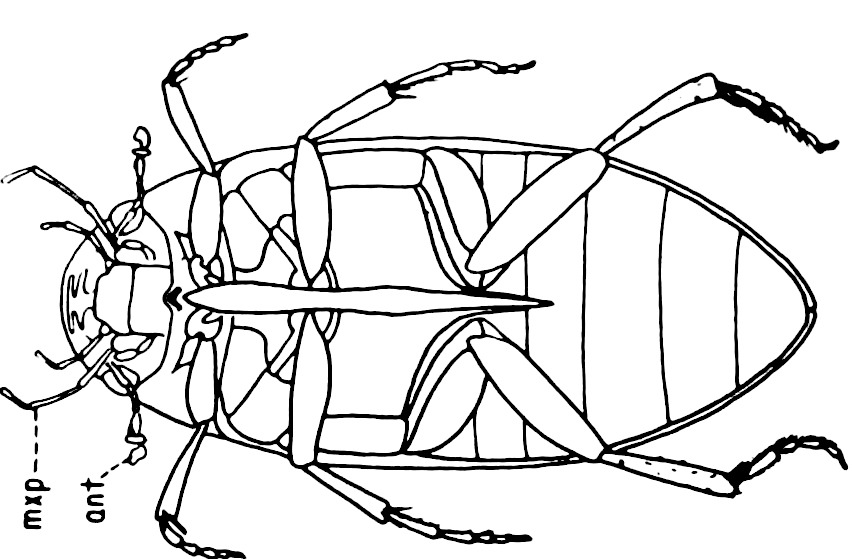
\includegraphics[angle=180,width=\textwidth]{coleopterida/Hydrophilid1}
  \caption{}
  \label{fig:hydrophilid1}
\end{subfigure}
    \qquad
\begin{subfigure}[ht!]{0.35\textwidth}
   \reflectbox{ 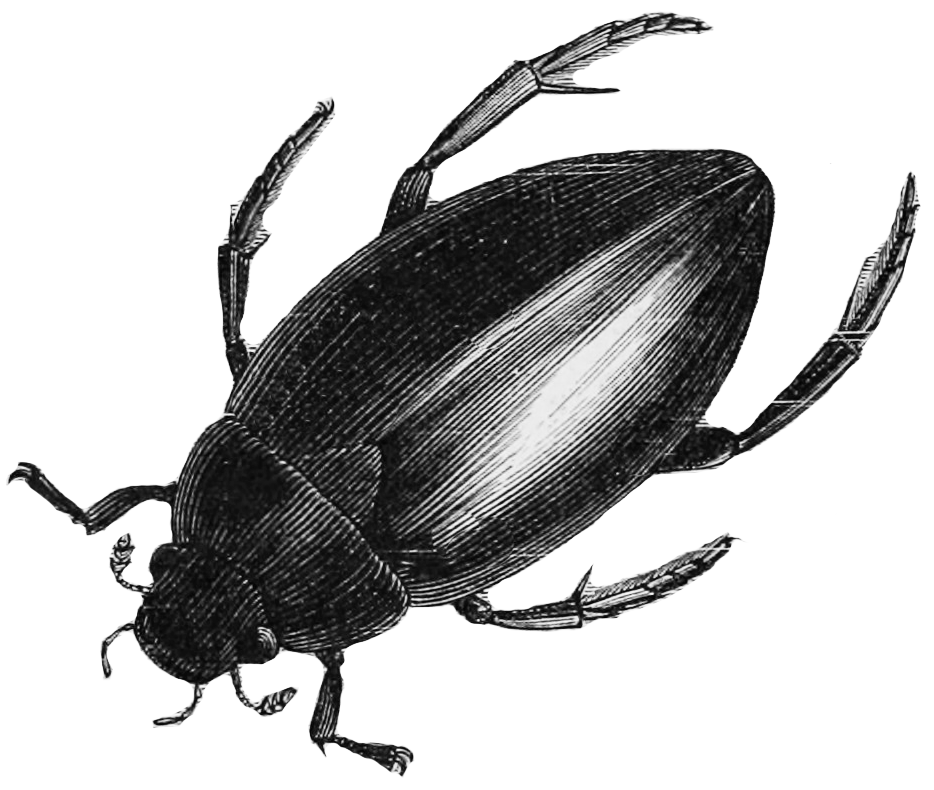
\includegraphics[width=\textwidth]{coleopterida/hydrophilidDorsal}}
  \caption{}
  \label{fig:hydrophilid2}
\end{subfigure}
    \caption{Hydrophilidae. \textbf{(a)} Ventral habitus \citep[][Fig. Fig. 13:36]{bhlitem126080aquatic}; \textbf{(b)} dorsal habitus \citep[][pg. 99]{brehm1877brehms}}\label{fig:hydrophilids}
\end{figure}

\subsubsection{Histeridae (clown beetles)}\index{Histeridae}
\noindent{}\textit{Diagnostic characters:} Elytra short, exposing 2 rigid tergites; body usually somewhat flattened to very flattened; antennae geniculate (elbowed), with distinct 3-segmented club; hind coxae widely separated and without distinct posterior face.\vspace{3mm}

\noindent{}\textit{Natural history:} Almost 4,000 species have been described worldwide, and all are thought to be predators of other insects. Like many staphylinids, some species are inquiline-predators in the nests of ants and termites.

\begin{figure}[ht!]
  \centering
    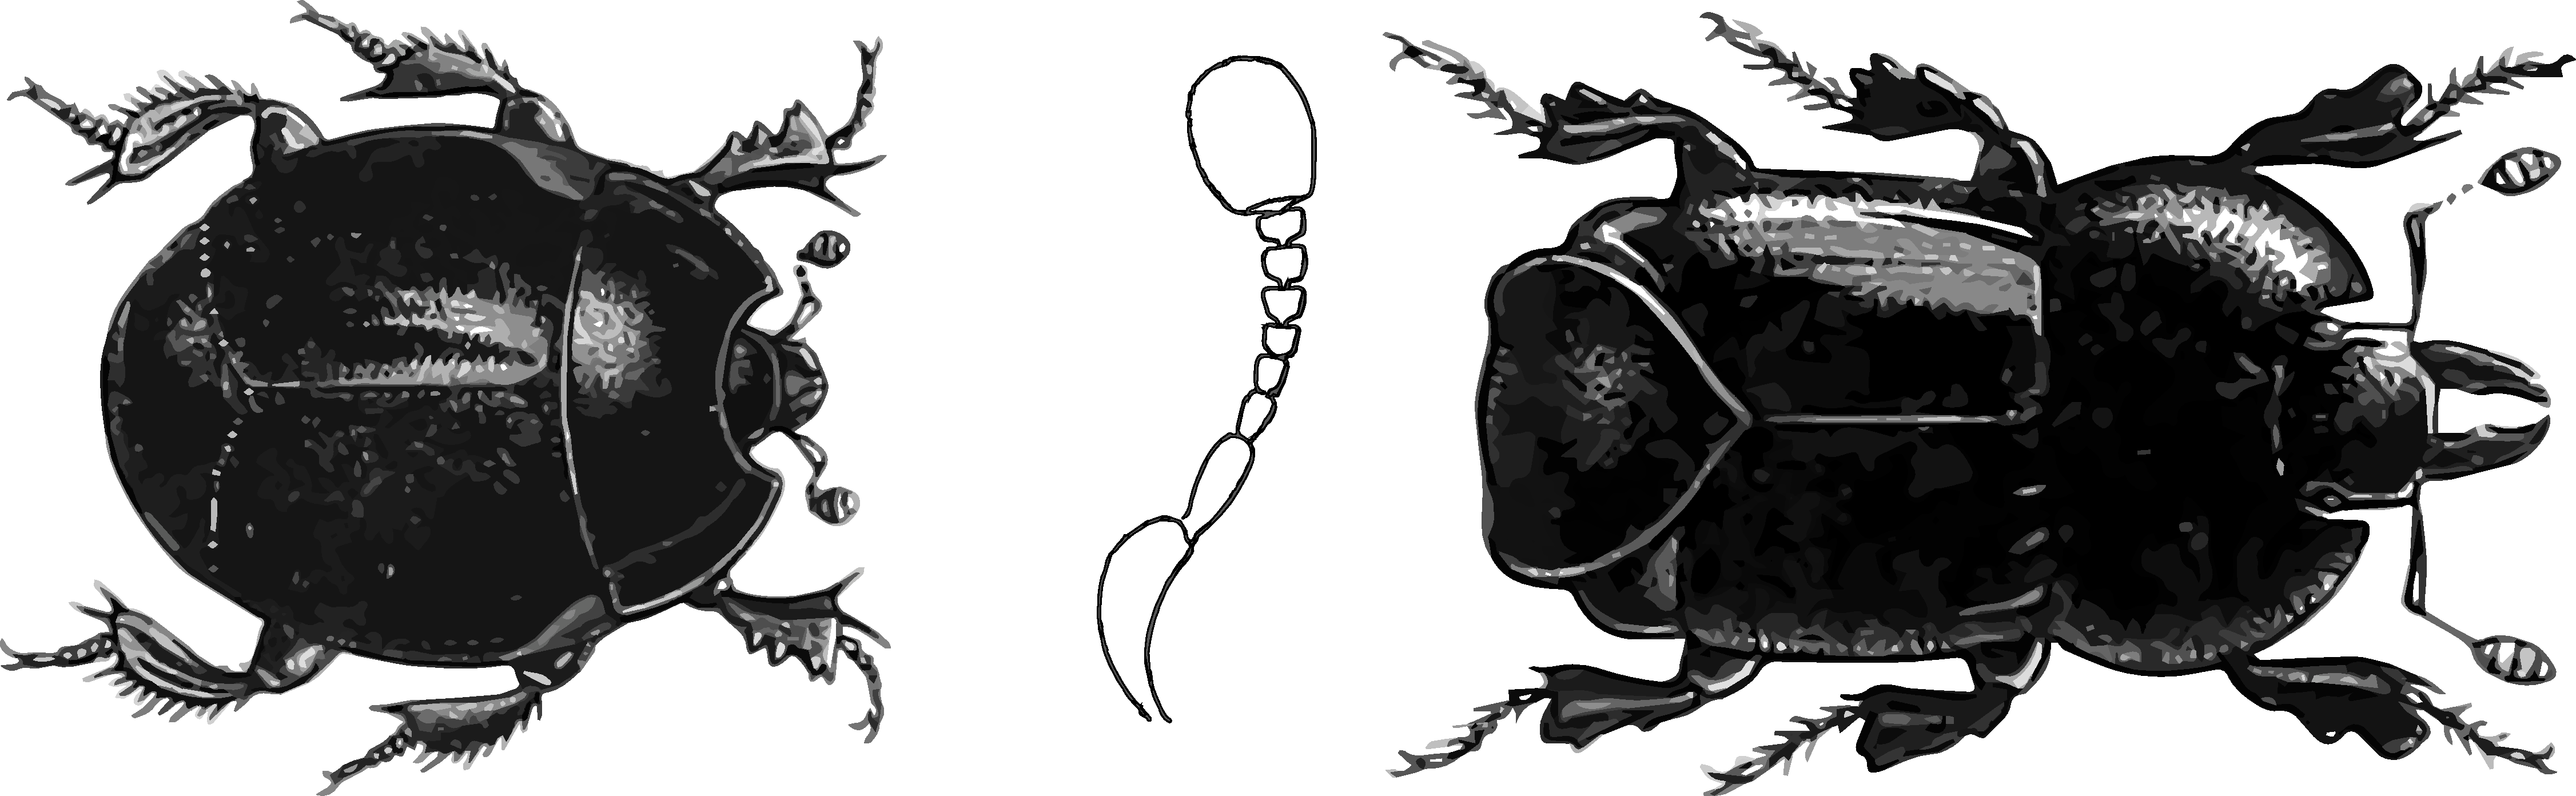
\includegraphics[width=0.75\textwidth]{coleopterida/histerids}
  \caption{Histeridae \citep[modified from][Plate 21, Figs. 20,22]{bhlitem240513beetles}}
  \label{fig:histerid}
\end{figure}

\subsubsection{Scarabaeidae (scarab, dung beetles, chafers)}\index{Scarabaeidae}
\noindent{}\textit{Diagnostic characters:} Antennae with asymmetrical lamellate, 3--4 merous club which can close tightly [Note that several families we don't cover in lab, \textit{e.g.}, Geotrupidae, have similar antennae!]; morphologically diverse, but abdomen with 6 sternites; fore legs often fossorial.\vspace{3mm}

\noindent{}\textit{Natural history:} Extraordinarily diverse family, with about 30,000 described species. Most are saprophages, feeding in decaying vegetation/wood, dung, \textit{etc}. The subfamily Dynastinae (Rhinoceros beetles) includes many large, popular, well-known species, as does Cetoniinae (Goliath Beetles). Males often have cranial or pronotal evaginations that serve as fighting instruments.

\begin{theo}
{}We've looked at several beetle families now. Why does each have an expanded mesoscutellum? They don't use their fore wings much for flight.
\end{theo}

\begin{figure}[ht!]
  \centering
    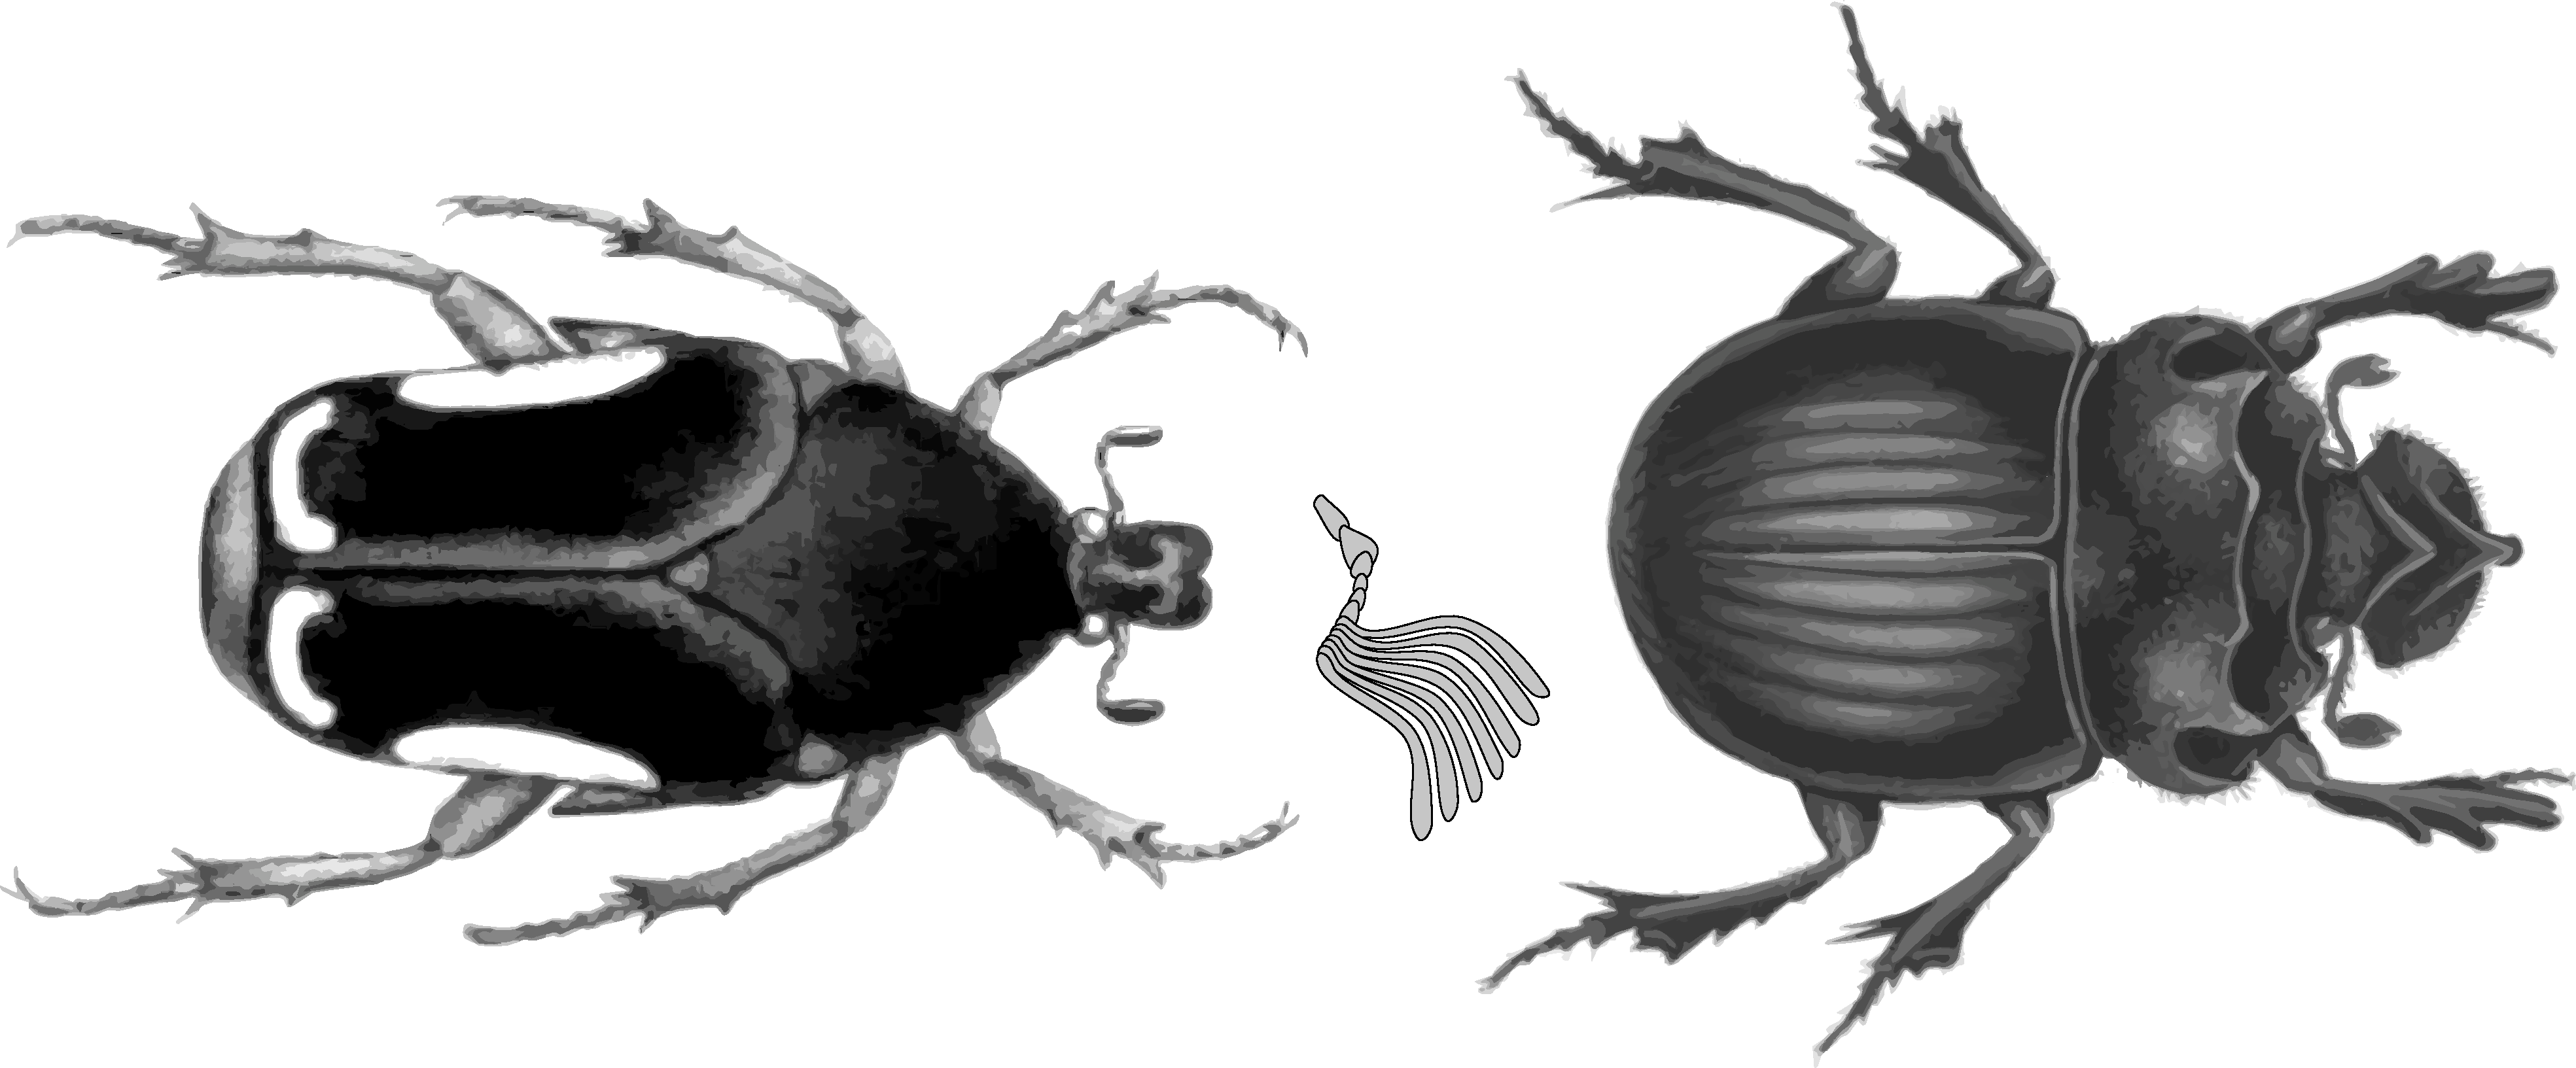
\includegraphics[width=0.75\textwidth]{coleopterida/Scarabaeidae}
  \caption{Scarabaeidae. L to R: dorsal habitus \citep[redrawn from][Plate V, Fig. 5]{bhlitem86018scarab}; lamellate antenna (vector drawing (CC BY-SA 4.0 International) by M. A. Broussard); dorsal habitus \citep[redrawn from plate in][]{bhlitem290909scarab}}
  \label{fig:scarabaeids}
\end{figure}

\subsubsection{Passalidae (bess or patent leather beetles)}\index{Passalidae}
\noindent{}\textit{Diagnostic characters:} Antennae with asymmetrical lamellate 3--6 merous club which does not close; sternites enclose mid coxal cavity, epimera not adjacent to coxal cavity; body elongate, parallel-sided, flattened, striated/grooved; head often with horn (figure \ref{fig:passalid}); very little morphological variation within this family.\vspace{3mm}

\noindent{}\textit{Natural history:} Approximately 500 species are known worldwide, most of which are found in the tropics. These beetles are known to exhibit subsocial behavior, living in colonies in rotten wood, where adults care for larvae over an extended period of time. Like termites, these beetles need to re-acquire gut symbionts after each molt.

\begin{figure}[ht!]
  \centering
    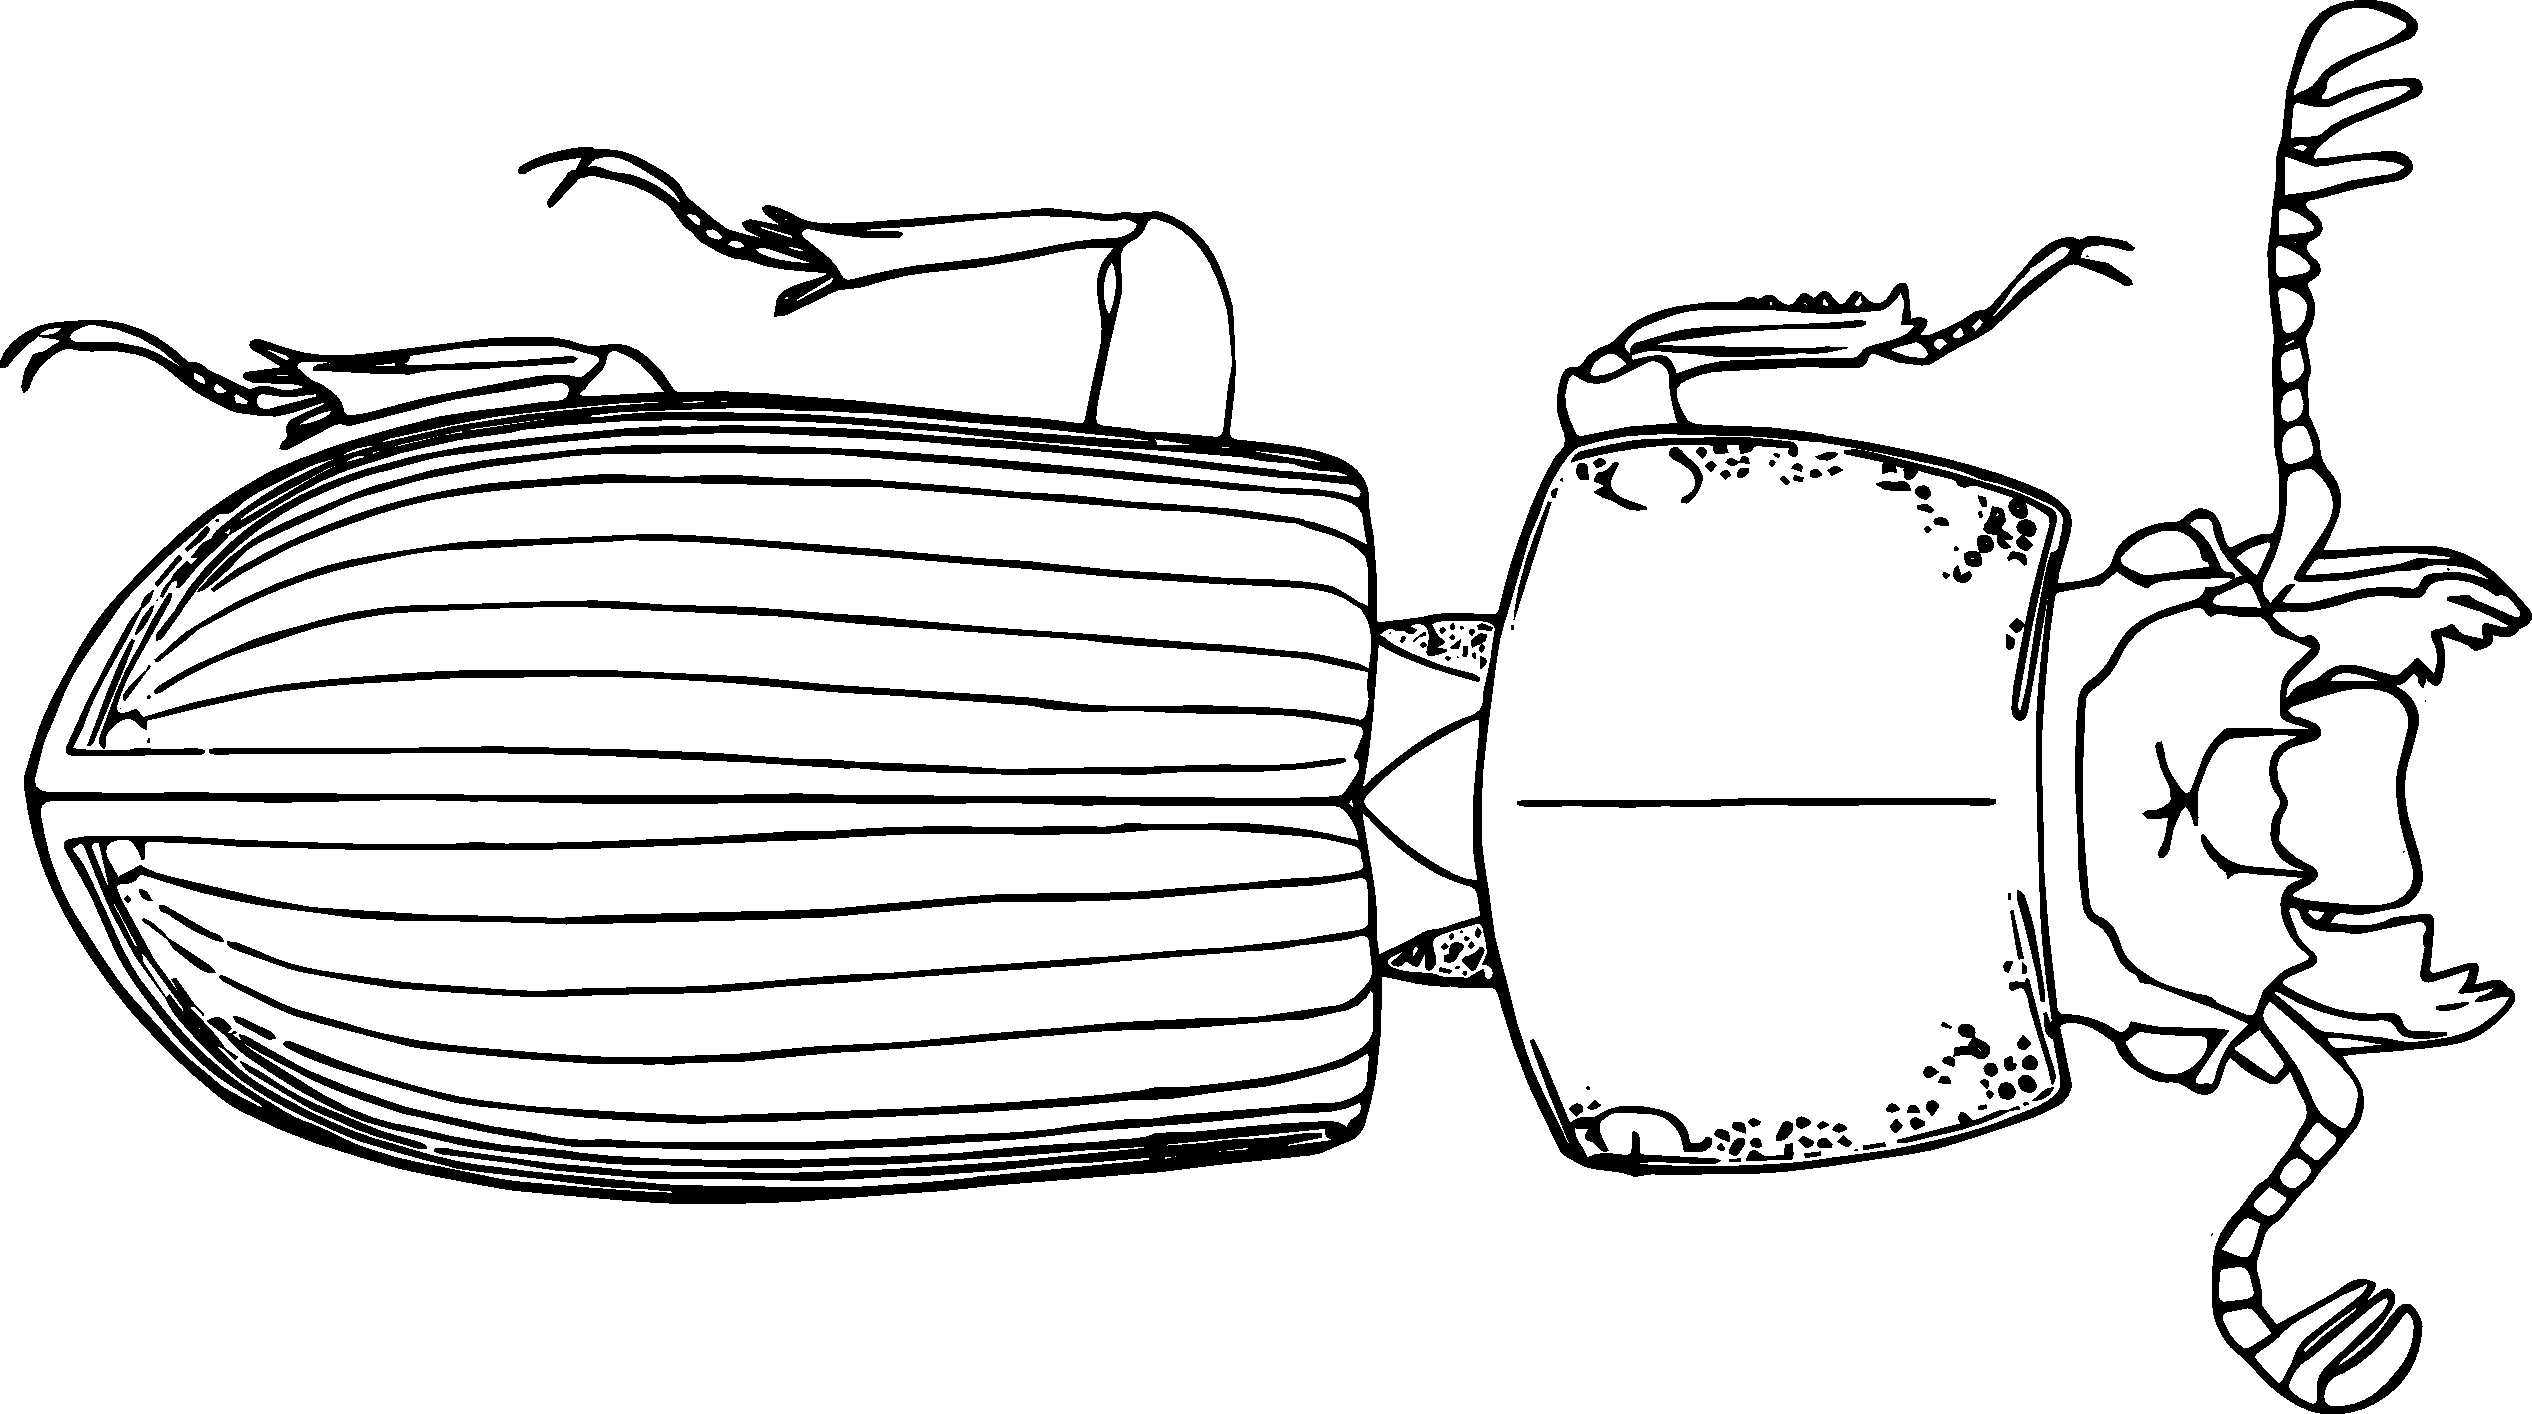
\includegraphics[width=0.5\textwidth]{coleopterida/PassalidHabitus}
  \caption{Passalidae \citep[redrawn from][Fig. 1A]{bhlitem38036beetles}}
  \label{fig:passalid} 
\end{figure}

\subsubsection{Lucanidae (stag beetles)}\index{Lucanidae}
\noindent{}\textit{Diagnostic characters:} Antennae often elbowed; with asymmetrical lamellate, 3--4 merous club which can not close completely; sternites do not enclose mid coxal cavity, epimera adjacent to coxal cavity; body not dorso-ventrally flattened, not striated; mandibles often very large.\vspace{3mm}

\noindent{}\textit{Natural history:} Approximately 1,200 species have been described worldwide, almost all of which feed on rotting wood. Males are well-known for ``fighting'' each other with over-sized mandibles.

\begin{figure}[ht!]
  \centering
    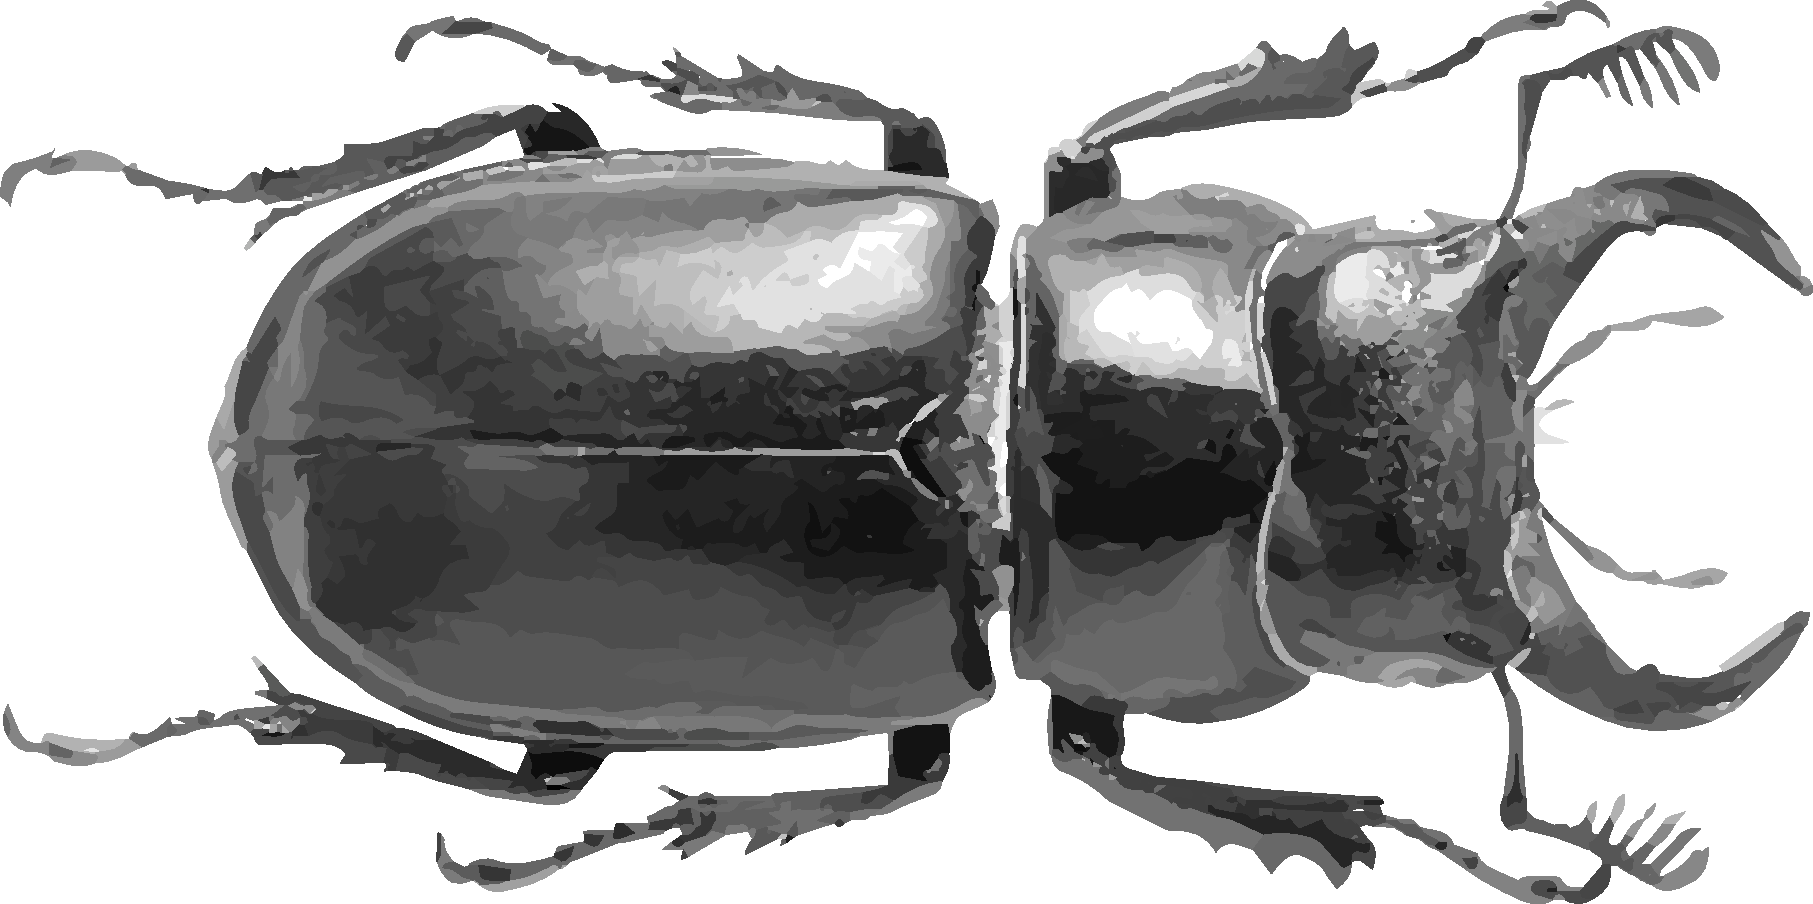
\includegraphics[width=0.55\textwidth]{coleopterida/Lucanidae}
  \caption{Lucanidae \citep[drawn from][Fig. 1F]{Lucanus2017}}
  \label{fig:lucanid1}%https://flic.kr/p/Dy1Eiv
\end{figure}

\subsubsection{Lycidae (net-winged beetles)}\index{Lycidae}
\noindent{}\textit{Diagnostic characters:} Abdomen with 7--8 visible sternites; elytra broad, flexible, reticulate, with network of ridges, usually broadest posteriorly; pronotum flattened, usually with strong median ridge, usually covering head; mid coxae separated far apart; femora and tibiae often flattened; antennae usually saw-toothed, occasionally thread-like.\vspace{3mm}

\noindent{}\textit{Natural history:} A diverse family, with \textgreater4,500 described species worldwide. Most species are understood to be fungivores as larvae, and adults will feed on nectar and honeydew. Many species are toxic and are aposematically colored and/or involved in mimicry complexes.

\begin{figure}[ht!]
  \centering
    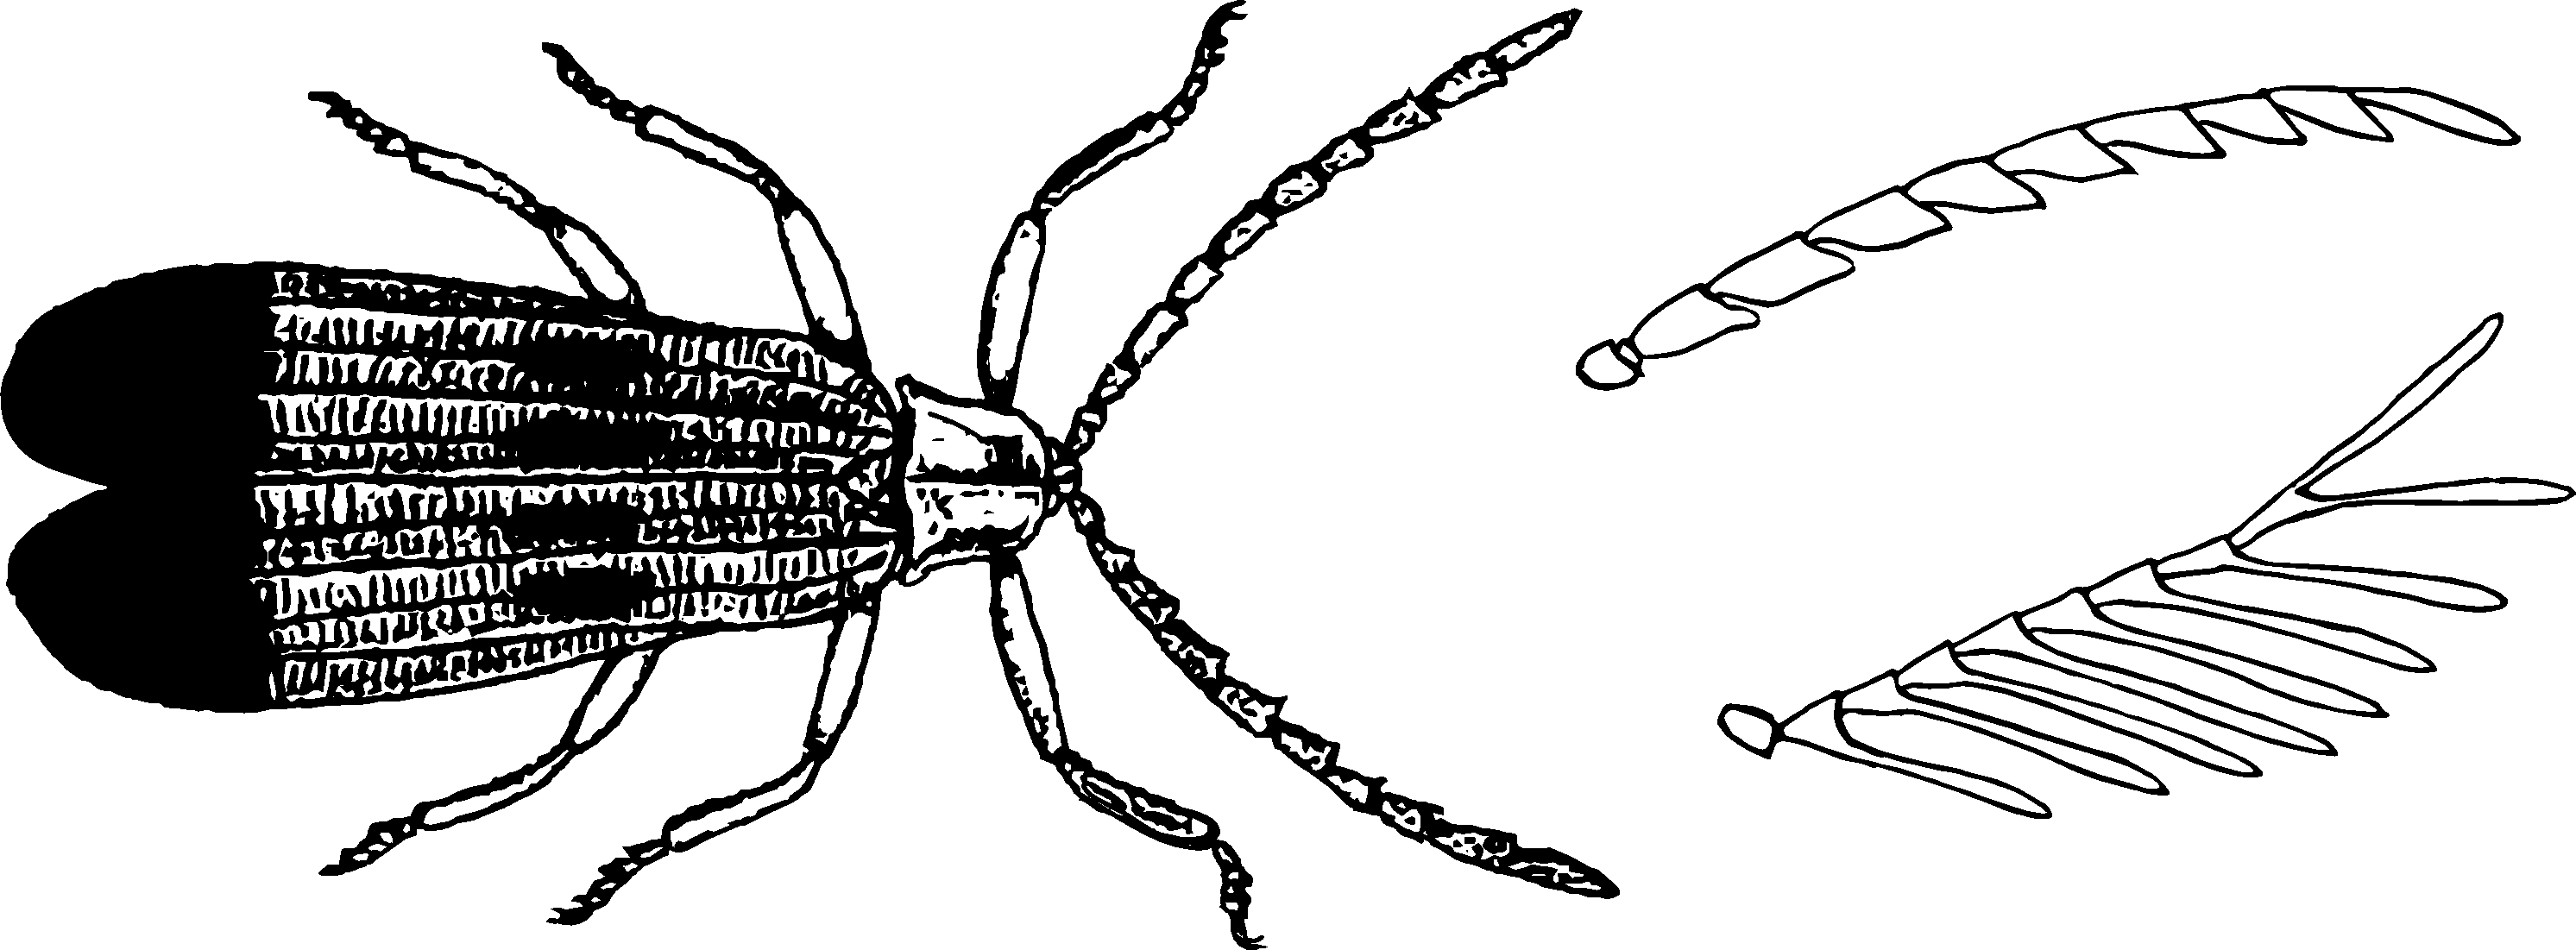
\includegraphics[width=0.7\textwidth]{coleopterida/Lycidae}
  \caption{Lycidae \citep[redrawn from][Plate V, Fig. 9]{bhlpart243991} }
  \label{fig:lycid}
\end{figure}

\subsubsection{Lampyridae (fireflies)}\index{Lampyridae}
\noindent{}\textit{Diagnostic characters:} Tarsi sometimes pseudotetramerous; abdomen with 7--8 visible sternites; antennae thread-like to saw-toothed; body and elytra soft, ridged but not reticulate, nearly parallel-sided, fairly elongate; head concealed from above by flattened pronotum; antennal insertions very close to each other; often with prominent luminescent organs.\vspace{3mm}

\noindent{}\textit{Natural history:} Approximately 2,000 species of lampyrids are known, many of which are bioluminescent as larvae and/or adults. Larvae are generally predators of other invertebrates, while adults may also feed on nectar and pollen. These beetles are generally toxic.

\begin{figure}[ht!]
  \centering
\begin{subfigure}[ht!]{0.42\textwidth}
    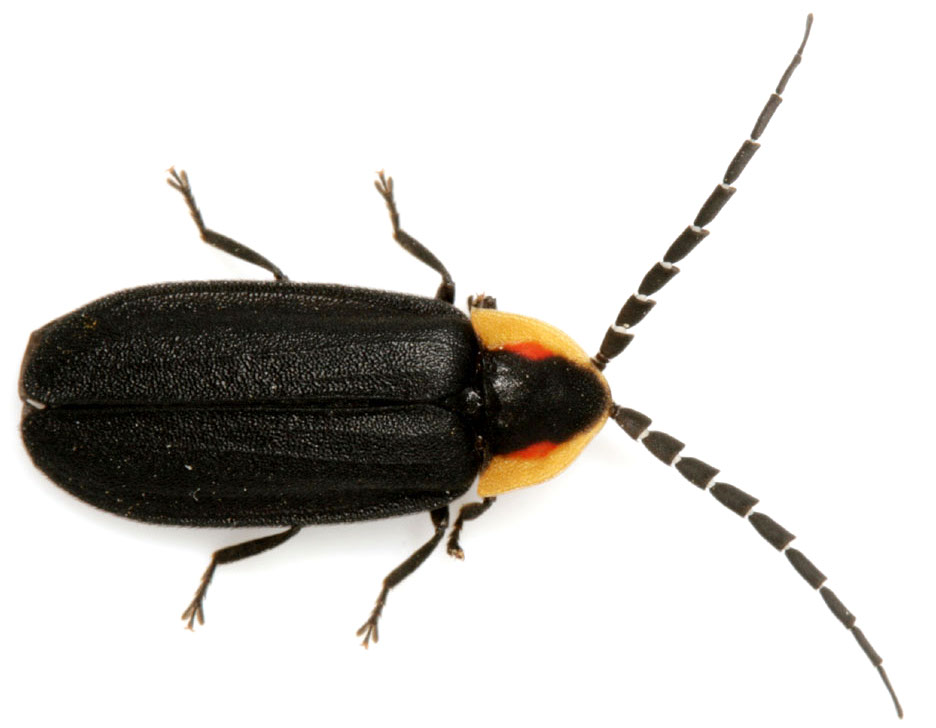
\includegraphics[width=\textwidth]{coleopterida/LampyridHabitus}
  \caption{}
  \label{fig:lampyrid1}
\end{subfigure}
    \qquad
\begin{subfigure}[ht!]{0.3\textwidth}
    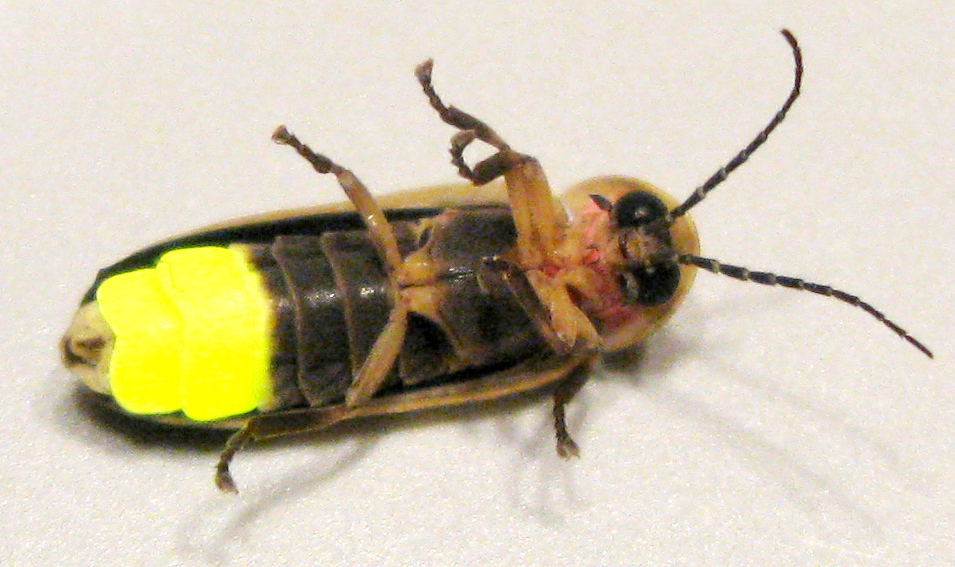
\includegraphics[width=\textwidth]{coleopterida/LampyridHabitusVentral}
  \caption{}
  \label{fig:lampyrid2}\end{subfigure}
    \caption{Lampyridae. \textbf{(a)} Dorsal habitus \citep[modified from][Tab. 4, Fig. 22]{bhlitem14605}; \textbf{(b)} ventral habitus (photo CC BY 2.0 by Andy Deans)}\label{fig:lampyrids}
\end{figure}

\subsubsection{Cantharidae (soldier beetles)}\index{Cantharidae}
\noindent{}\textit{Diagnostic characters:} Abdomen with 7--8 visible sternites; antennae usually long, threadlike to saw-toothed; similar to Lampyridae (soft-bodies, elongate, \textit{etc}.), but: head usually not completely concealed from above; legs long; most of femur usually visible dorsally; antennal insertions further apart; no luminescent organ.\vspace{3mm}

\noindent{}\textit{Natural history:} Cantharid larvae develop as predators of other insects, especially eggs and larvae. Adult diets also may include pollen and nectar. More than 5,000 species have been described worldwide. bhlitem14605

\begin{figure}[ht!]
  \centering
    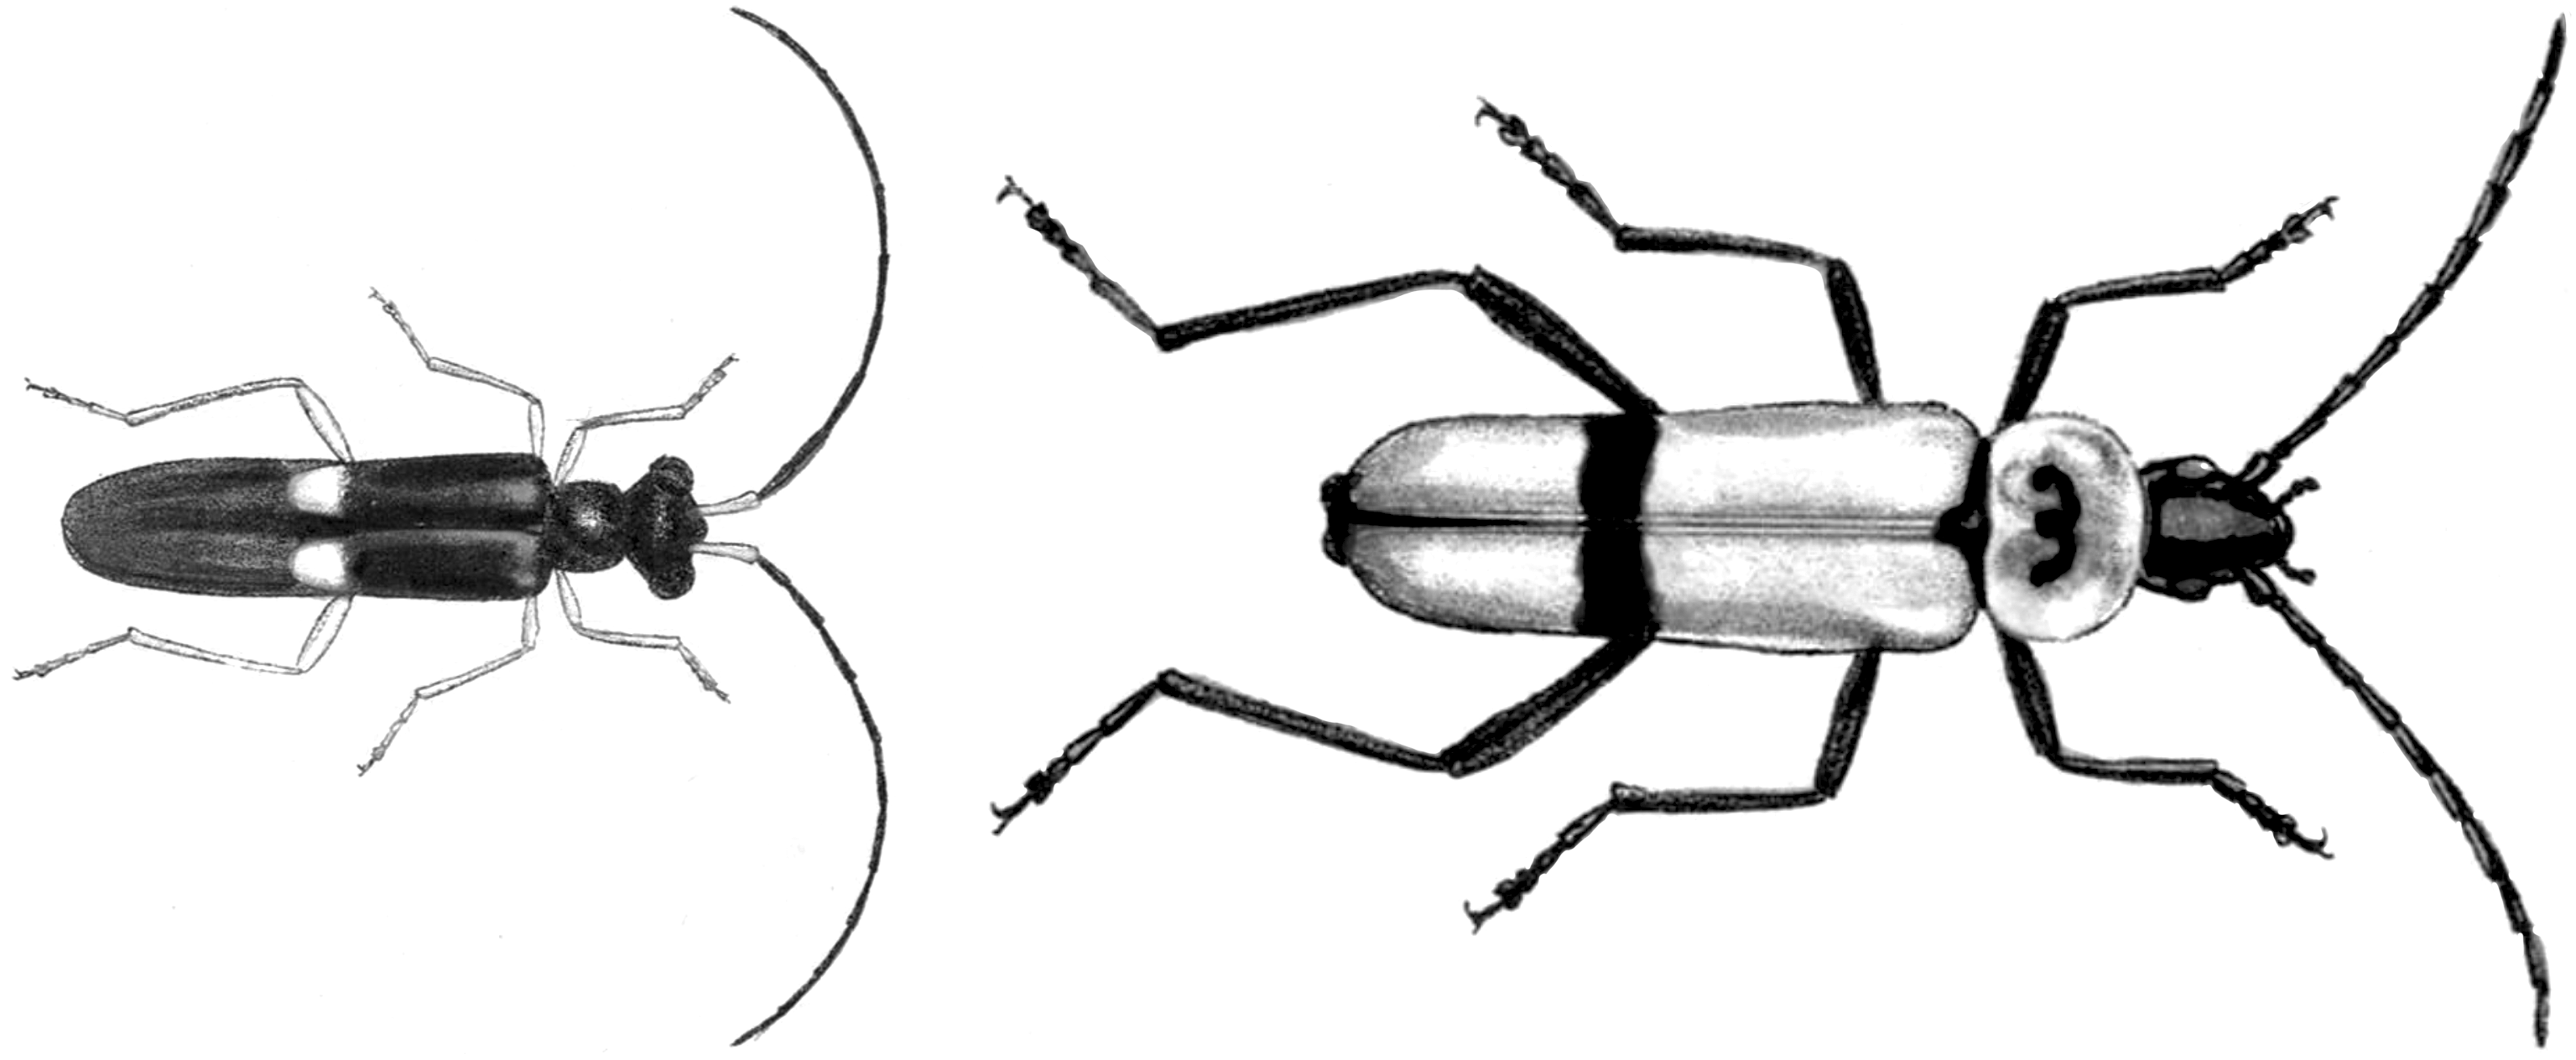
\includegraphics[width=0.8\textwidth]{coleopterida/cantharids}
  \caption{Cantharidae, dorsal habitus \cite[redrawn from][Plate 6, Fig. 14; plate 5, Fig. 11]{bhlitem14605}}
  \label{fig:cantharids}
\end{figure}

\subsubsection{Elateridae (click beetles)}\index{Elateridae}
\noindent{}\textit{Diagnostic characters:} Abdomen with 6 or fewer visible sternites; pronotal processes pointed posteriorly; prosternum has elongated lobe (clicking mechanism); antennae saw-toothed (occasionally comb-like), never clubbed; body elongate, narrow and parallel or tapering.\vspace{3mm}

\noindent{}\textit{Natural history:} The number of described click beetles is approaching 10,000 worldwide. Most species are capable of flipping their bodies via the click mechanism (prosternal process, clicking into mesosternal scrobe). Larvae typically develop as saprophages or predators, while adults are usually herbivores.\vspace{3mm}

\begin{figure}[ht!]
  \centering
    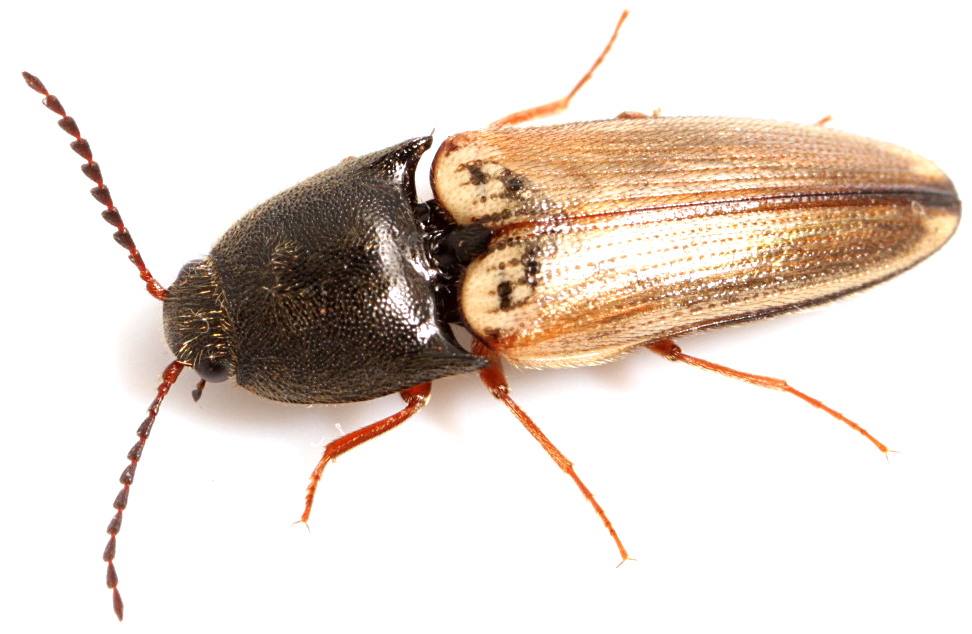
\includegraphics[width=0.8\textwidth]{coleopterida/ElateridHabitus}
  \caption{Elateridae habitus (right), with ventral view of prothoracic click mechanism (left) \cite[redrawn from][Plate 18, Fig. 21a; plate 15, Fig. 9a; Plate 12, Fig. 9]{bhlitem14604}}
  \label{fig:elaterids}
\end{figure}

\subsubsection{Dermestidae (carpet beetles)}\index{Dermestidae}
\noindent{}\textit{Diagnostic characters:} Abdomen with 6 or fewer visible sternites; mid coxal cavity always open; fore coxae usually conical; pronotum mostly conceals head dorsally; antennae short, with abrupt 3-merous club, often fitting into grooves in pronotum; elytra often patterned with scales or small hairs; body robust, elongate-oval to round.\vspace{3mm}

\noindent{}\textit{Natural history:} Approximately 600 species are known worldwide. All are scavengers of plant or animal materials, and several species are pests in museum collections.

\begin{figure}[ht!]
  \centering
\begin{subfigure}[ht!]{0.4\textwidth}
    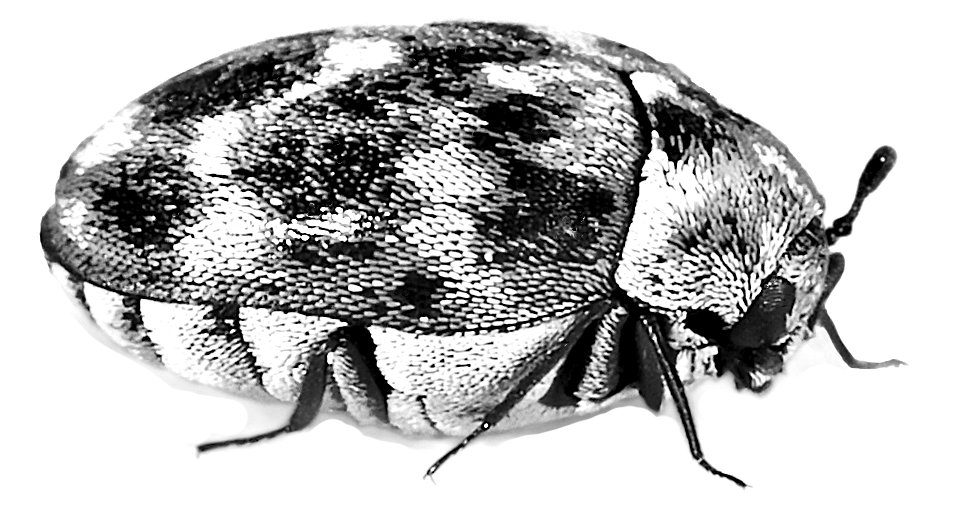
\includegraphics[width=\textwidth]{coleopterida/DermestidHabitus}
  \caption{}
  \label{fig:dermestid1}
\end{subfigure}
\hfill
\begin{subfigure}[ht!]{0.45\textwidth}
    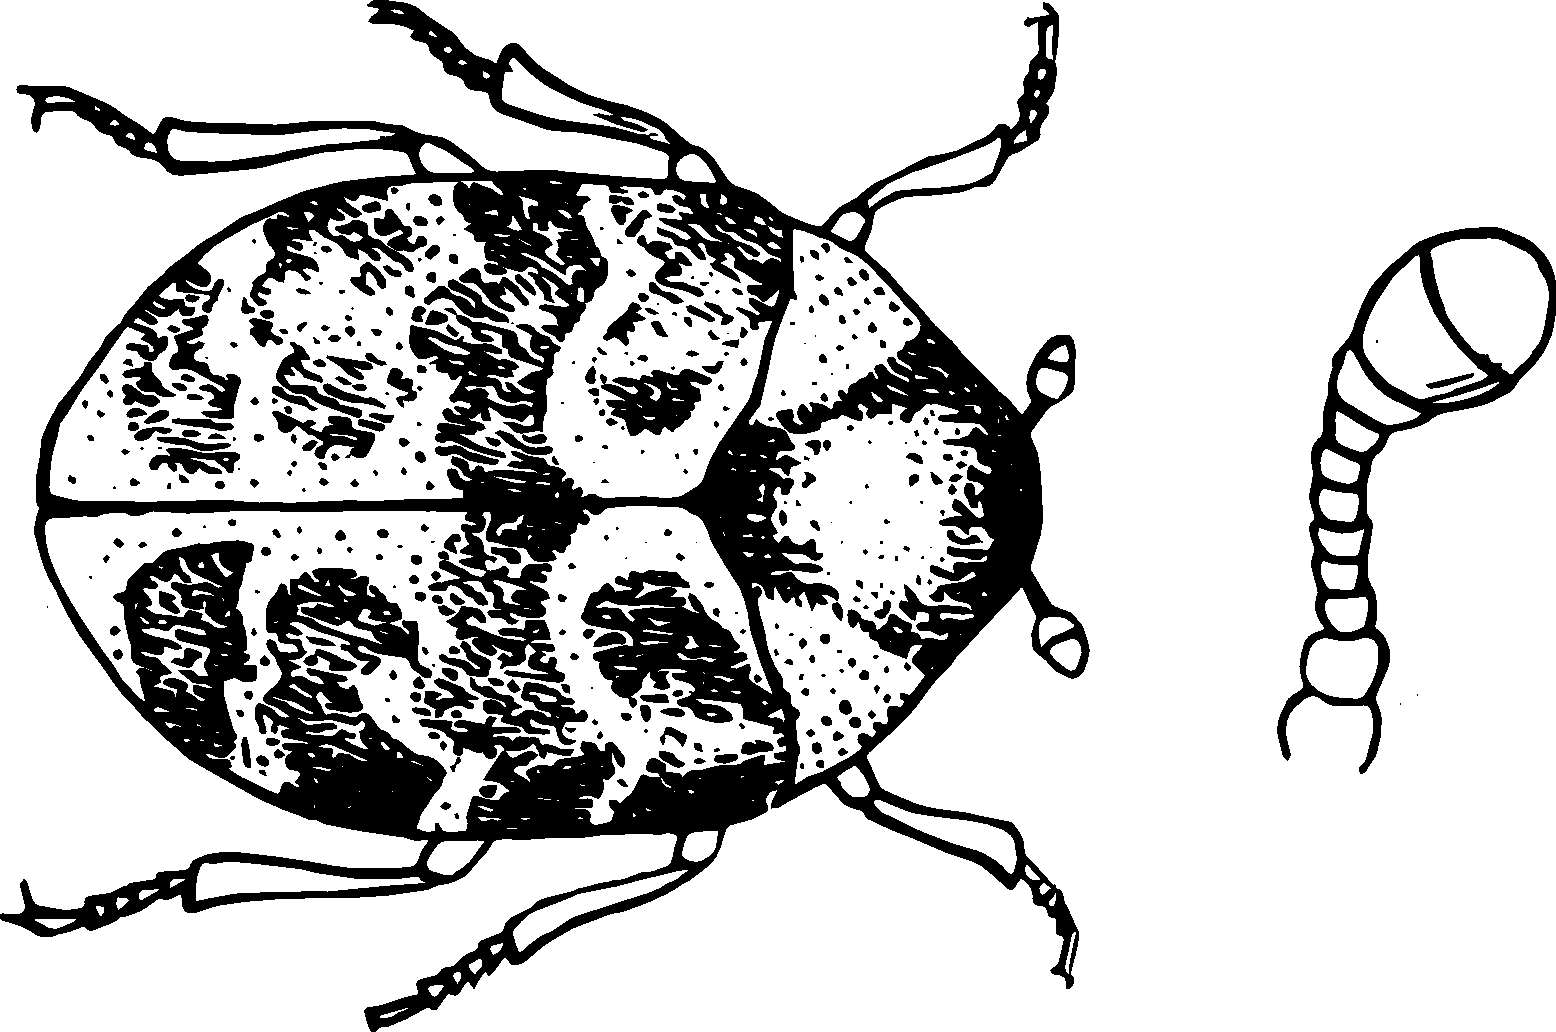
\includegraphics[width=\textwidth]{coleopterida/Dermestidae}
  \caption{}
  \label{fig:dermestid2}\end{subfigure}
    \caption{Dermestidae. \textbf{(a)} Lateral habitus (modified from photo (CC BY-SA 4.0 International) by Didier Descouens \url{https://goo.gl/HwFCZA}); \textbf{(b)} dorsal habitus \citep[redrawn from][Plate 35, Fig. 7]{bhlitem37317beetles}}\label{fig:dermestid}
\end{figure}

\subsubsection{Buprestidae (metallic wood-boring beetles)}\index{Buprestidae}
\noindent{}\textit{Diagnostic characters:} Abdomen with 6 or fewer visible sternites; sternites do not enclose mid coxal cavity, epimera adjacent to coxal cavity; pronotum encircles head; antennae often short, rarely with 3-merous club; body narrow, distinctive shape, often metallic or shiny.\vspace{3mm}

\noindent{}\textit{Natural history:} These beetles are all herbivores as larvae and generally develop as borers of plants. Approximately 15,000 species have been described worldwide, including many important pests (\textit{e.g.}, Emerald Ash Borer; \textit{Agrilus planipennis} Fairmaire, 1888).

\begin{figure}[ht!]
  \centering
     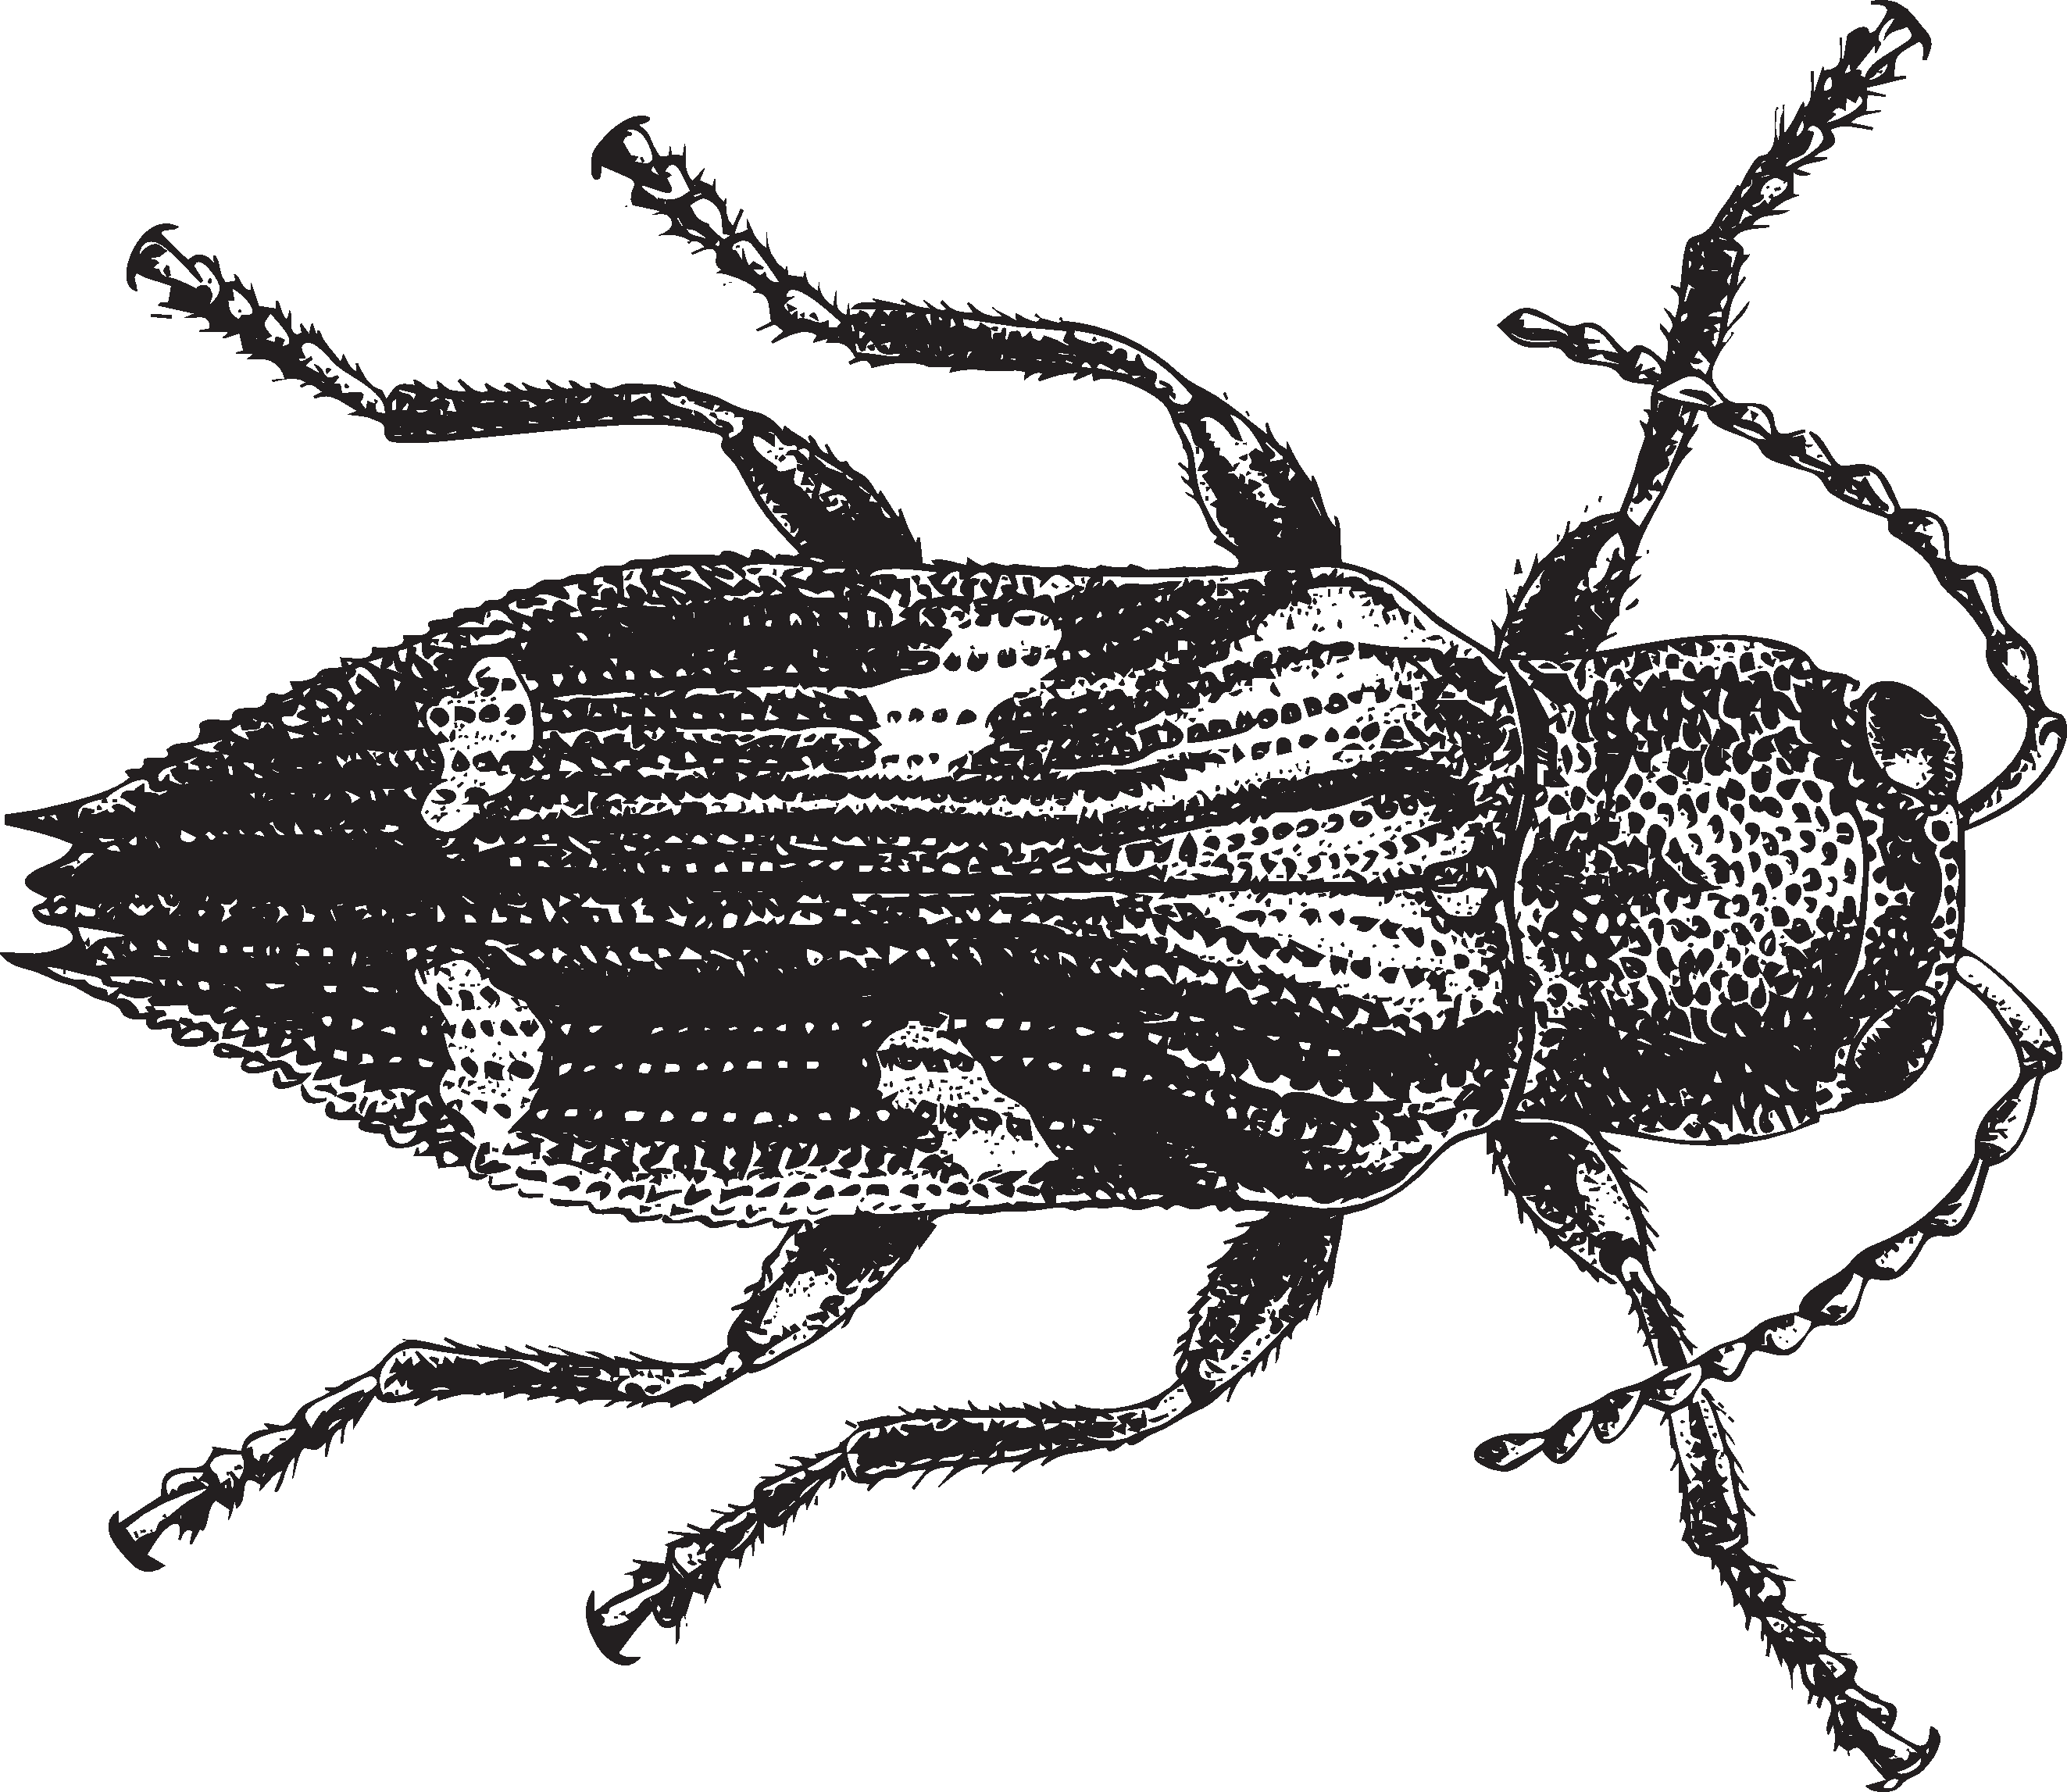
\includegraphics[width=0.45\textwidth]{sections/img/coleopterida/Buprestidae.pdf}
  \caption{Buprestidae habitus. Redrawn from habitus by A.C. Harris  \url{https://en.m.wikipedia.org/wiki/File:COLE_Buprestidae_Nascioides_enysi.png}}
  \label{fig:buprestid}
\end{figure}

\subsubsection{Bostrichidae (auger, powderpost beetles)}\index{Bostrichidae}
\noindent{}\textit{Diagnostic characters:} 1st tarsomere often very small; abdomen with 6 or fewer visible sternites; sternites enclose mid coxal cavity, epimera not adjacent to coxal cavity; prothorax hood-like, mostly concealing head from above, usually with rasp-like texture anteriorly; antennae with fairly compact 3--4-merous club; hind trochanter short, triangular; body well sclerotized, somewhat cylindrical; head bent down, usually concealed from above.\vspace{3mm}

\noindent{}\textit{Natural history:} These beetles usually feed in living or dead/dried wood as larvae. Some species feed on woody fungi. Approximately 600 species are known worldwide.

\begin{figure}[ht!]
  \centering
     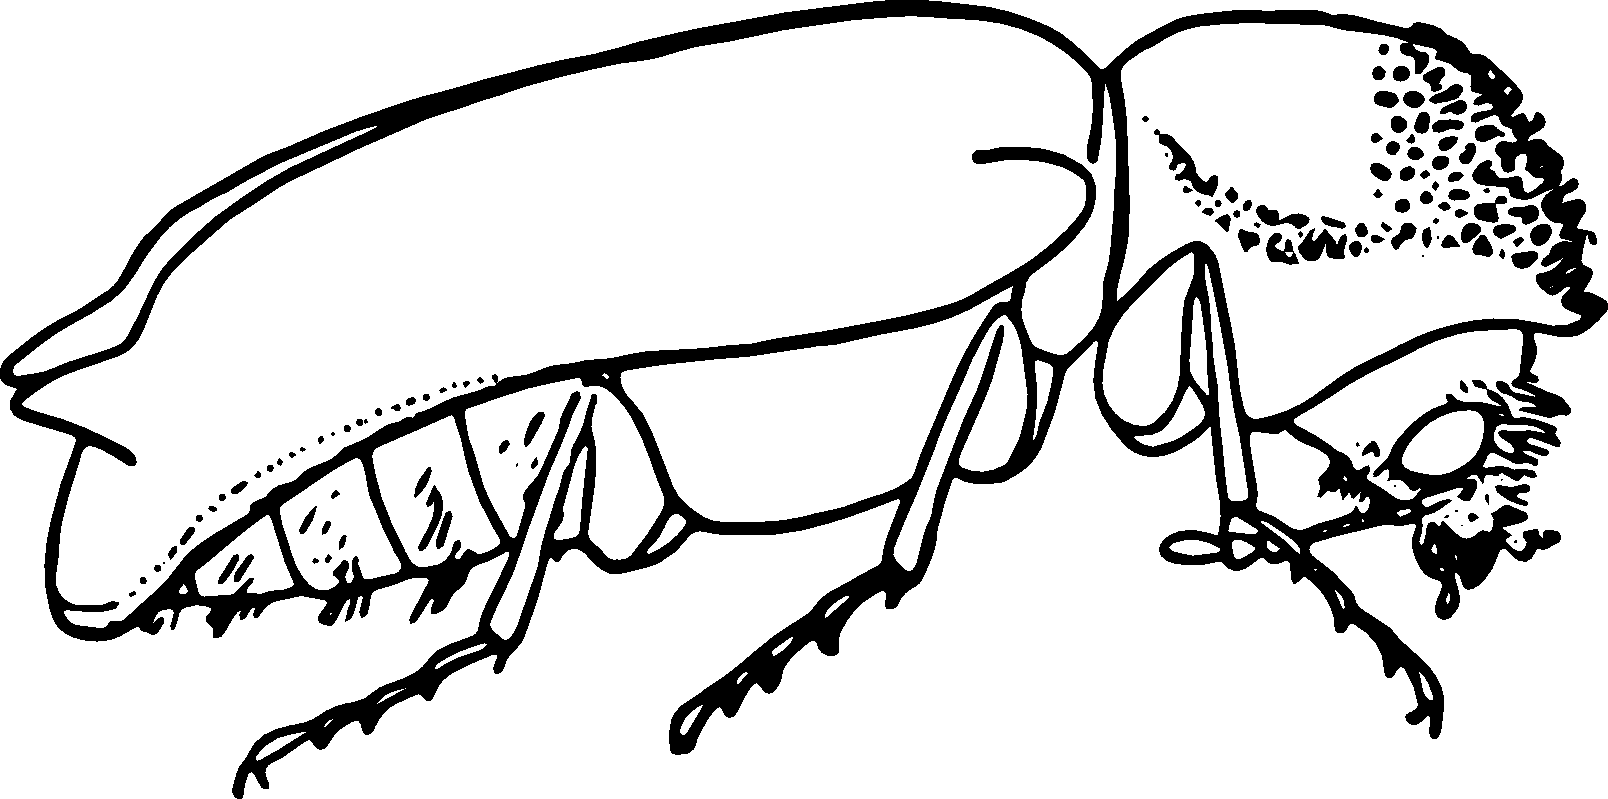
\includegraphics[width=0.4\textwidth]{sections/img/coleopterida/bostrichid}
  \caption{Bostrichidae habitus \citep[redrawn from][Fig. 183b]{bhlitem92397}}
  \label{fig:bostrichid}
\end{figure}

\begin{figure}[ht!]
  \centering
     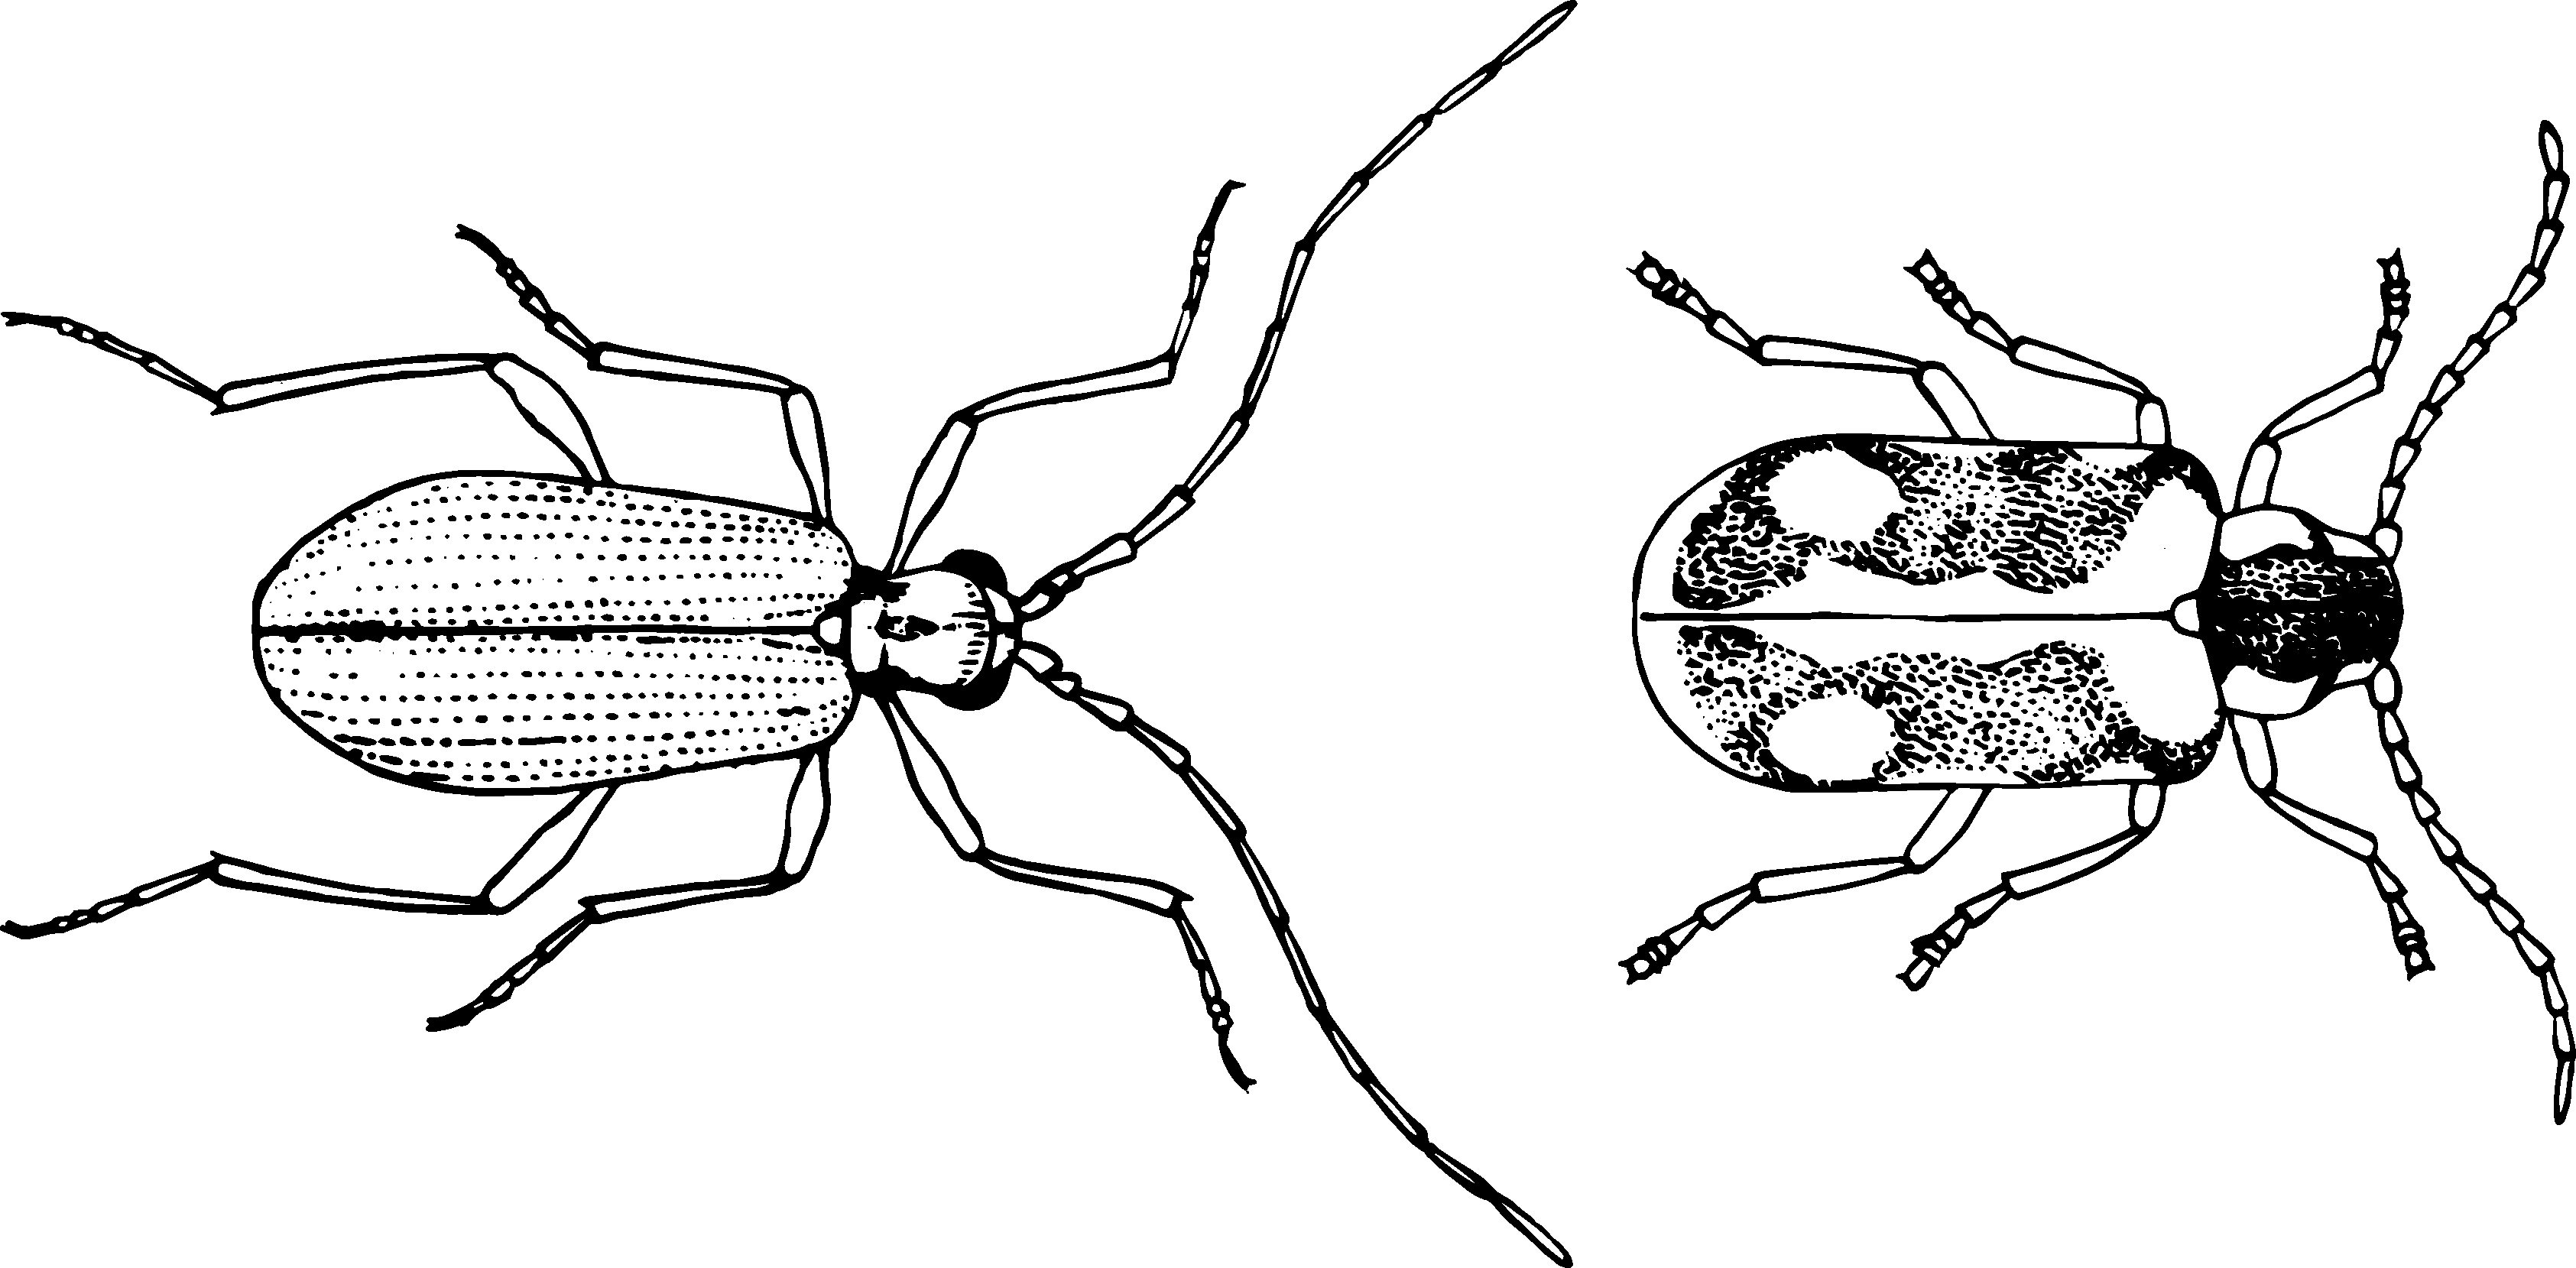
\includegraphics[width=0.65\textwidth]{sections/img/coleopterida/ptinids}
  \caption{Ptinidae habitus \citep[redrawn from][Plate 54, Figs 5,6]{bhlitem37317beetles}}
  \label{fig:anobiid}
\end{figure}

\subsubsection{Ptinidae (deathwatch, spider beetles)}\index{Ptinidae}
\noindent{}\textit{Diagnostic characters:} Abdomen with 6 or fewer visible sternites; sternites enclose mid coxal cavity, epimera not adjacent to coxal cavity; prothorax hood-like, partially enclosing head and concealing it from above; antennae with loose 3-merous club, sometimes comb-like; hind trochanter longer and cylindrical; head and appendages, particularly hind femur, can often be tucked into grooves (scrobes).\vspace{3mm}

\noindent{}\textit{Natural history:} Like bostrichids, these beetles typically bore in wood as larvae. Many species are pests of natural history and other museum collections and/or dried, stored products. The current name should probably be Ptinidae \citep{arango2012death}.

\begin{theo}
{}Many of these families (\textit{e.g}., Dermestidae, Bostrichidae, Ptinidae, and Tenebrionidae) have a \latinword{cryptonephridial system} that allows for efficient water recovery from the gut. Can you describe how such a system would be adaptive? In what situations can these beetles become pests?
\end{theo}

\subsubsection{Nitidulidae (sap beetles)}\index{Nitidulidae}
\noindent{}\textit{Diagnostic characters:} Fore coxa with exposed trochantin; hind coxa does not reach elytra; antennal club abrupt, ball-like, 3-merous; elytra usually not striate, usually shorter than abdomen; pronotum often covering part of head dorsally; body usually robust, sometimes very flattened- if very flat, not parallel-sided; similar to Erotylidae but usually smaller in size, with exposed hind trochantin and usually shortened elytra.\vspace{3mm}

\noindent{}\textit{Natural history:} These beetles typically feed on decaying vegetable matter and sap. More than 4,500 species have been described worldwide, including some pests of stored products.

\begin{figure}[ht!]
  \centering
\begin{subfigure}[ht!]{0.4\textwidth}
    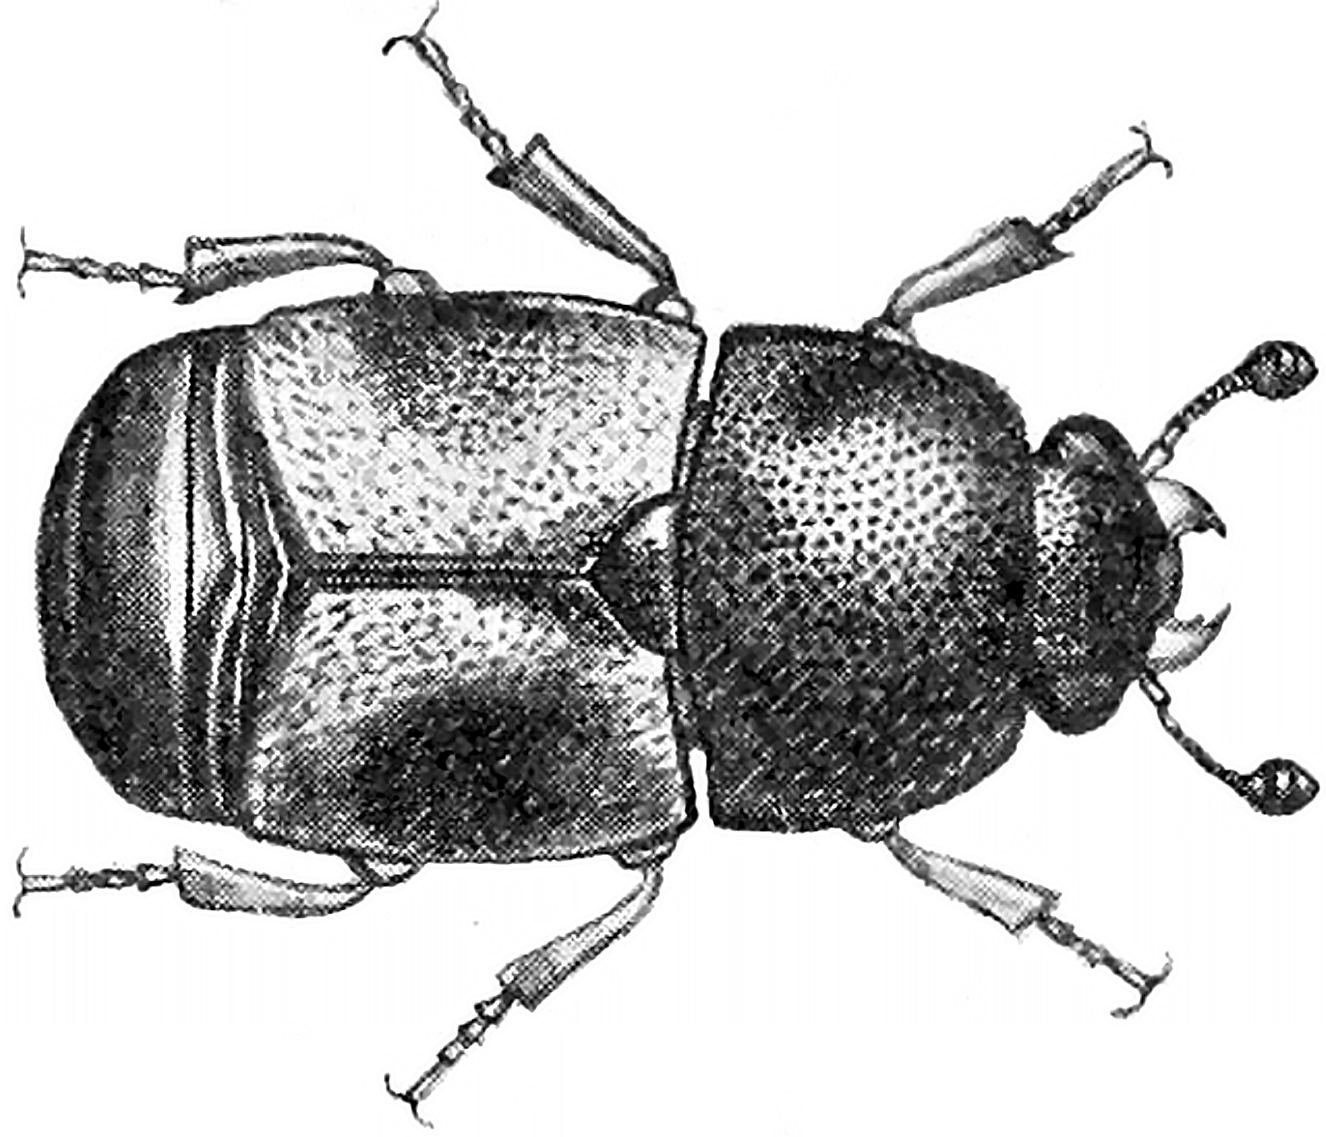
\includegraphics[width=\textwidth]{coleopterida/Nitidulidae}
  \caption{Nitidulidae}
  \label{fig:nitidulid}
\end{subfigure}
    \hfill
\begin{subfigure}[ht!]{0.46\textwidth}
    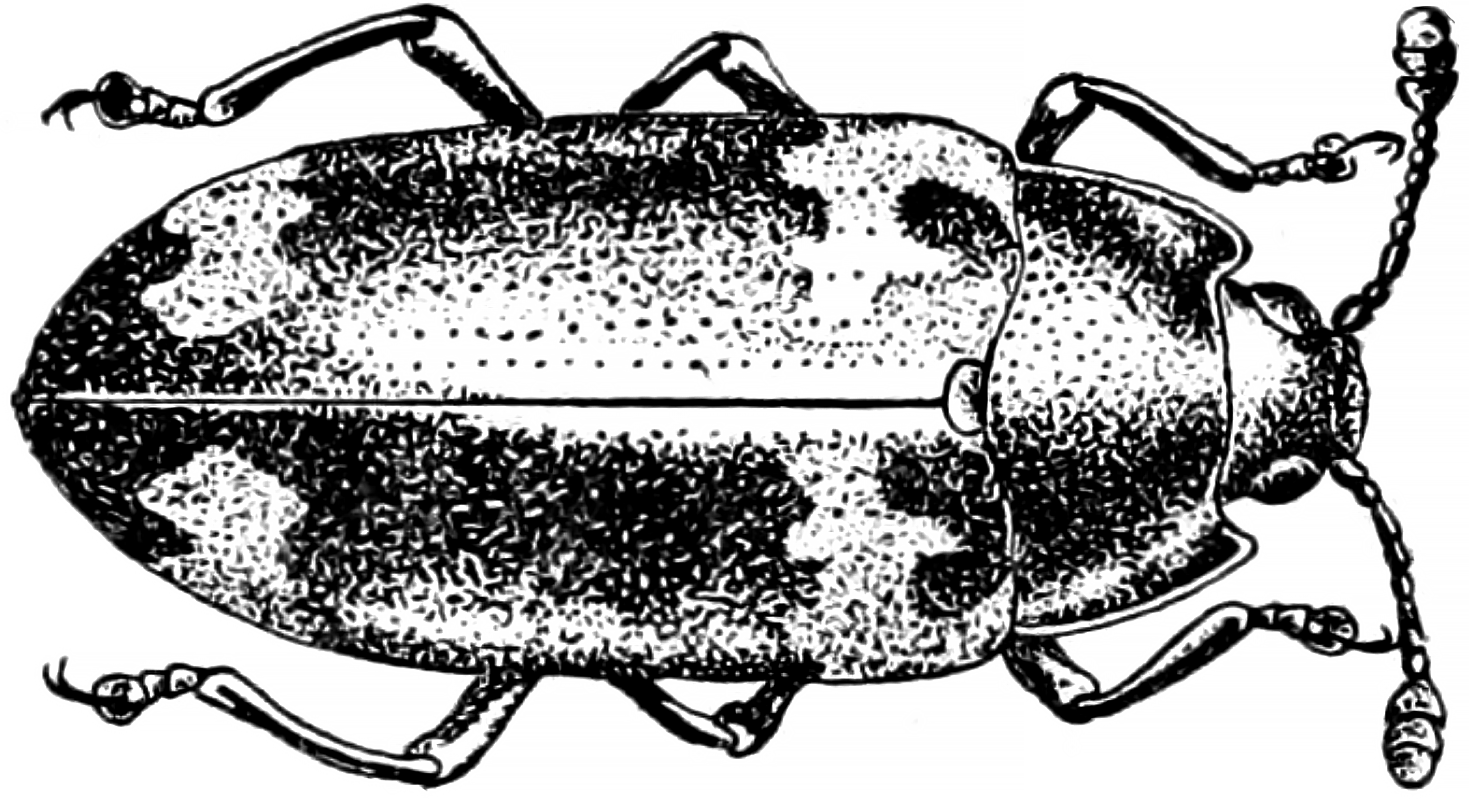
\includegraphics[width=\textwidth]{coleopterida/Erotylidae}
  \caption{Erotylidae}
  \label{fig:erotylid}\end{subfigure}
    \caption{\textbf{(a)} Nitidulidae habitus \citep[modified from][Fig. 71]{bhlitem64043}; \textbf{(b)} Erotylidae habitus \citep[modified from][Fig. 11]{heller1918beitrag}}\label{fig:erotylnitid}
\end{figure}

\subsubsection{Erotylidae (pleasing fungus beetles)}\index{Erotylidae}
\noindent{}\textit{Diagnostic characters:} Trochantin concealed or absent mid coxal cavity closed; antennae with abrupt 3--4-merous club; elongate-oval to oval, usually black and shiny and often with reddish or yellowish markings; similar to Nitidulidae but typically larger in size and with concealed or absent hind trochantin and elytra that usually cover whole abdomen.\vspace{3mm}

\noindent{}\textit{Natural history:} Larvae and adults feed on the fruiting bodies of fungi. About 3,500 species have been described worldwide.

\subsubsection{Mordellidae (tumbling flower beetles)}\index{Mordellidae}
\noindent{}\textit{Diagnostic characters:} Tarsi 5-5-4; body wedge-shaped humpbacked, forming a spine posteriorly; hind legs enlarged, hind tibia and tarsus with serrated ridges; antennae fairly short, threadlike or saw-toothed; head strongly retracted backwards.\vspace{3mm}

\noindent{}\textit{Natural history:} Approximately 1,500 species of this distinctive family have been described worldwide. Adults, which are typically found on flowers, escape disturbance by jumping repeatedly (``tumbling'') until they can right themselves and fly. Larvae usually bore in plants of fungi.

\begin{figure}[ht!]
  \centering
    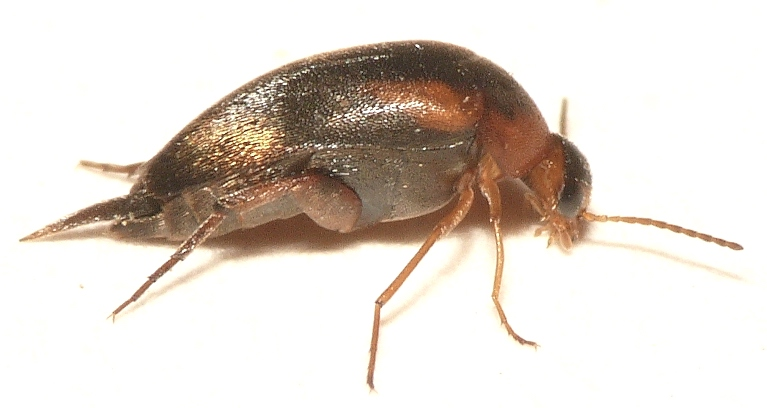
\includegraphics[width=0.5\textwidth]{coleopterida/MordellidHabitus}
  \caption{Mordellidae habitus. Photo (CC BY-SA 2.0) by Udo Schmidt, via Wikimedia Commons}
  \label{fig:mordellid}
\end{figure}%need line drawing or black and white - https://commons.wikimedia.org/wiki/Category:Georgiy_Jacobson._Beetles_Russia_and_Western_Europe#/media/File:Jacobs81.jpg   https://commons.wikimedia.org/wiki/Category:The_Coleoptera_of_the_British_islands#/media/File:The_coleoptera_of_the_British_Islands_BHL22446192.jpg

\subsubsection{Meloidae (blister beetles)}\index{Meloidae}
\noindent{}\textit{Diagnostic characters:} Tarsi 5-5-4; claw of fore tarsus with large blade ventrally; head broad, wider than pronotum, with gradual constriction behind eyes; pronotum narrower than head and elytra; antennae slender, not clubbed; body soft, leathery, elytra ``loose'', sometime shorter than abdomen.\vspace{3mm}

\noindent{}\textit{Natural history:} Cleptoparasites or parasitoids of bees and other insects. The first instar larvae (``triungulins'') are very small and phoretic, hitching rides on their hosts while hanging out near flowers. Adults are capable of reflex bleeding toxic hemolymph from weaknesses in the conjunctiva. This hemolymph can cause blistering in humans. About 7,500 species are known worldwide.\vspace{3mm}

\noindent{}CAUTION: Specimens exude toxic chemicals (even after death!)

\begin{figure}[ht!]
  \centering
\begin{subfigure}[ht!]{0.45\textwidth}
    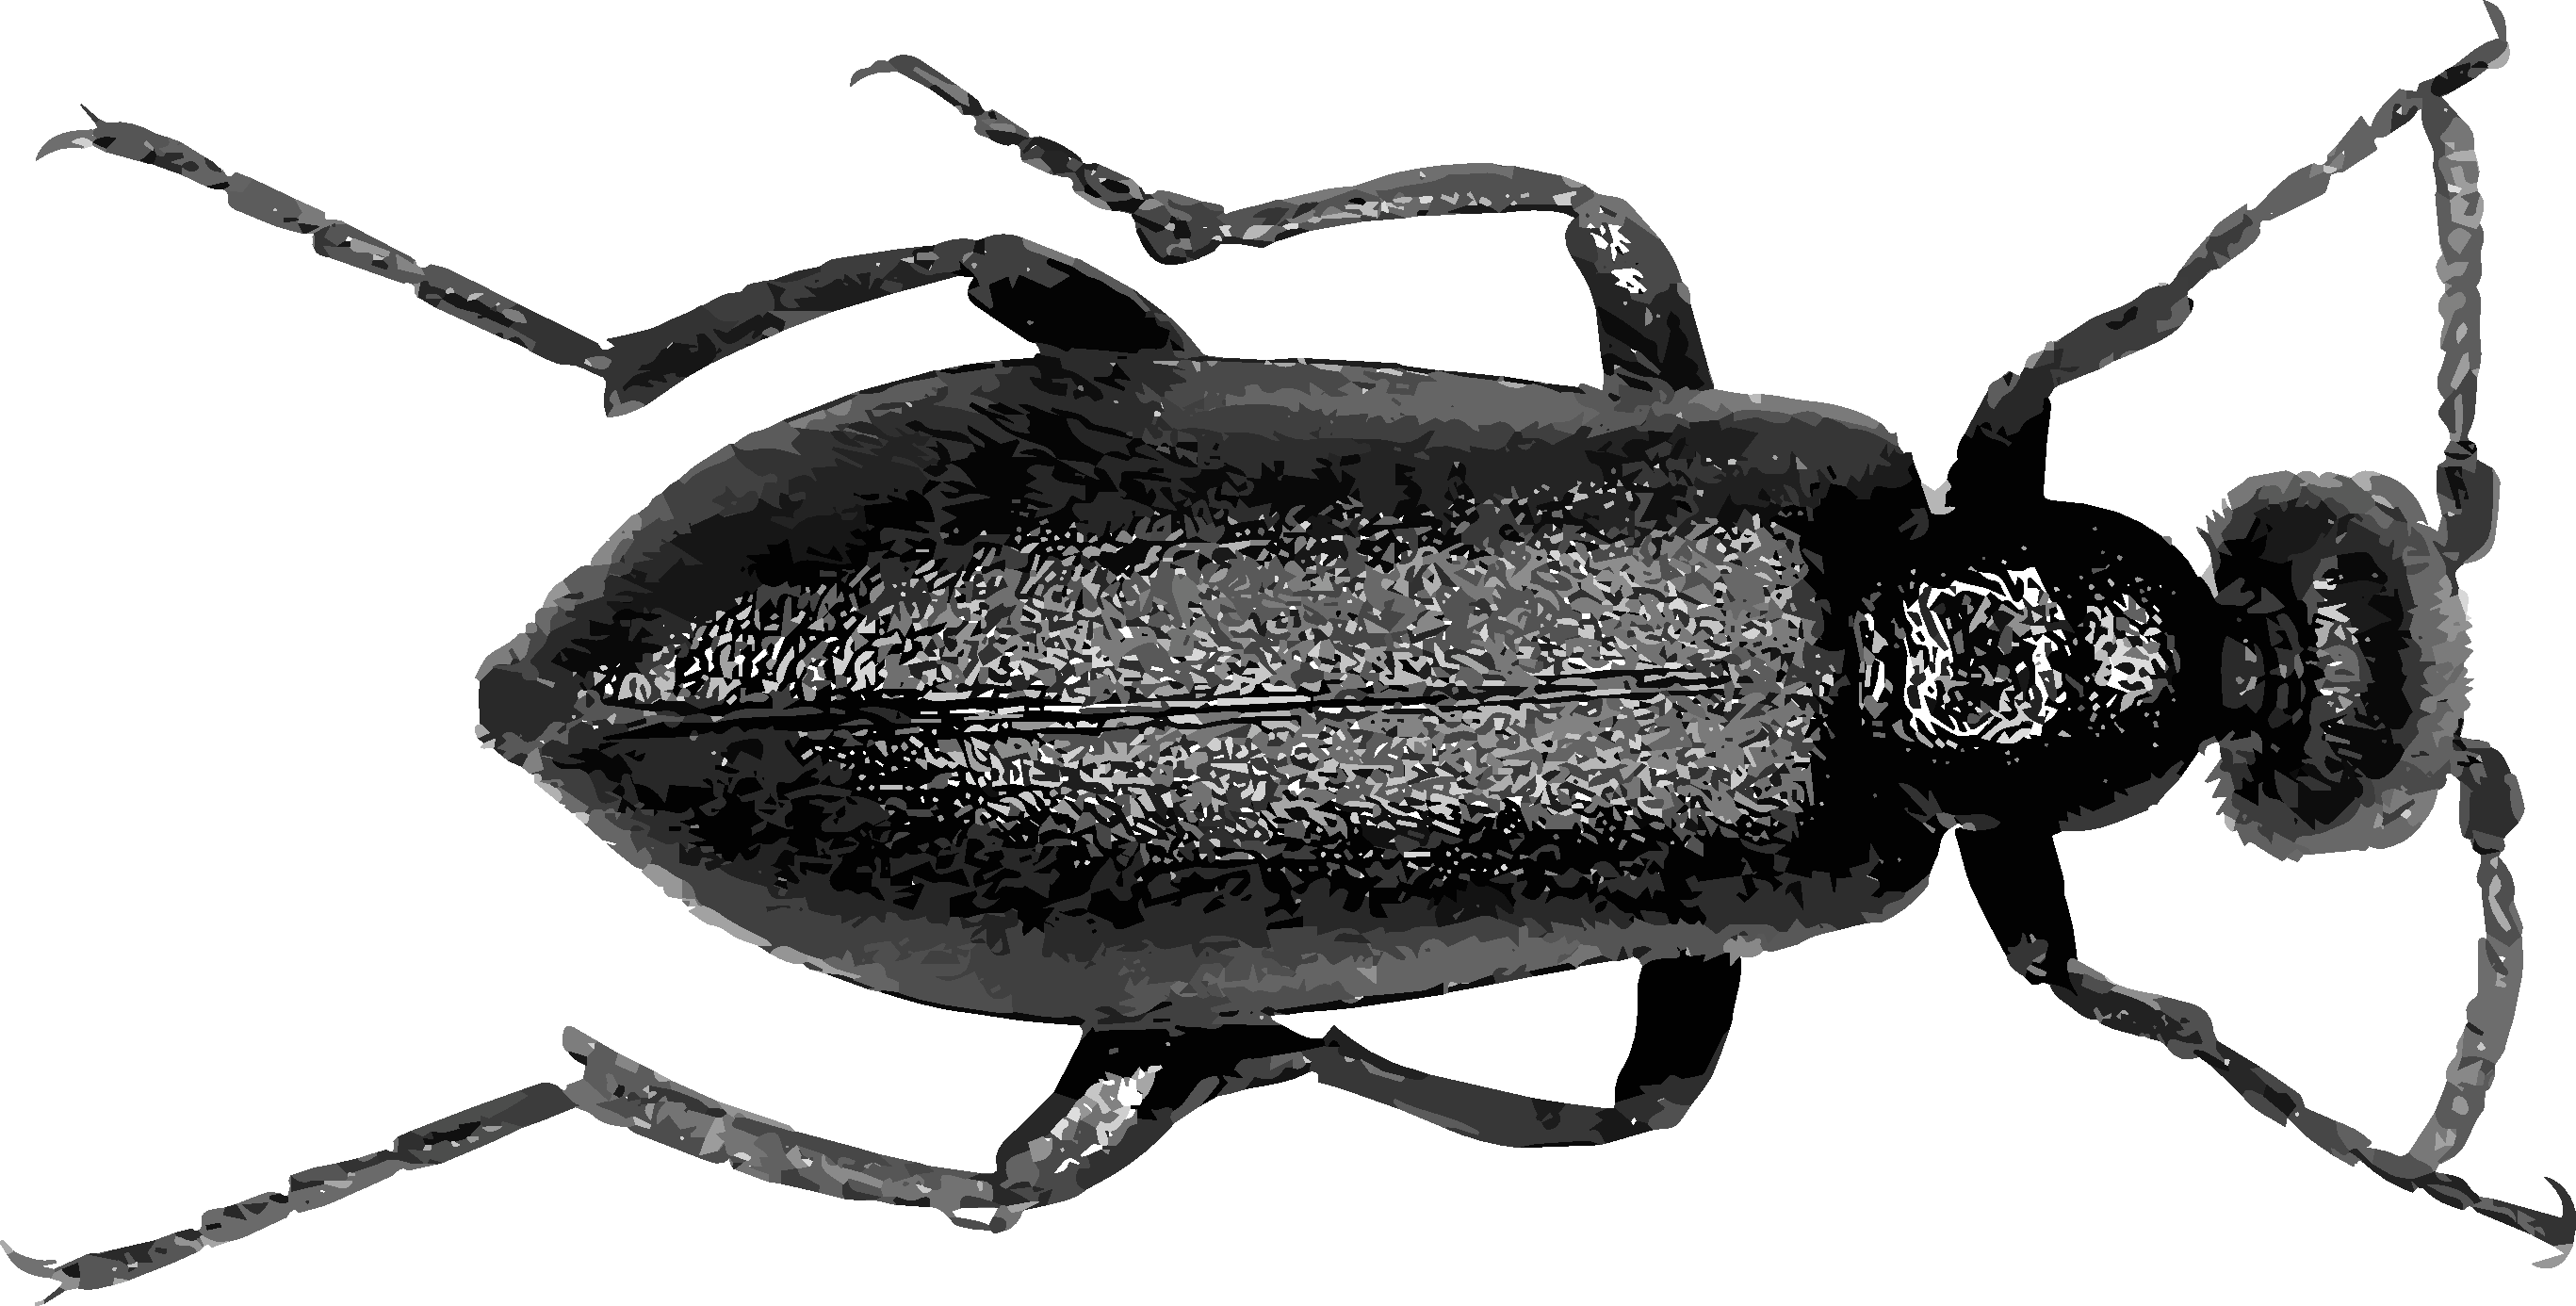
\includegraphics[width=\textwidth]{coleopterida/MeloidHabitus}
  \caption{Meloidae }
  \label{fig:meloid}
\end{subfigure}
    \hfill
\begin{subfigure}[ht!]{0.47\textwidth}
    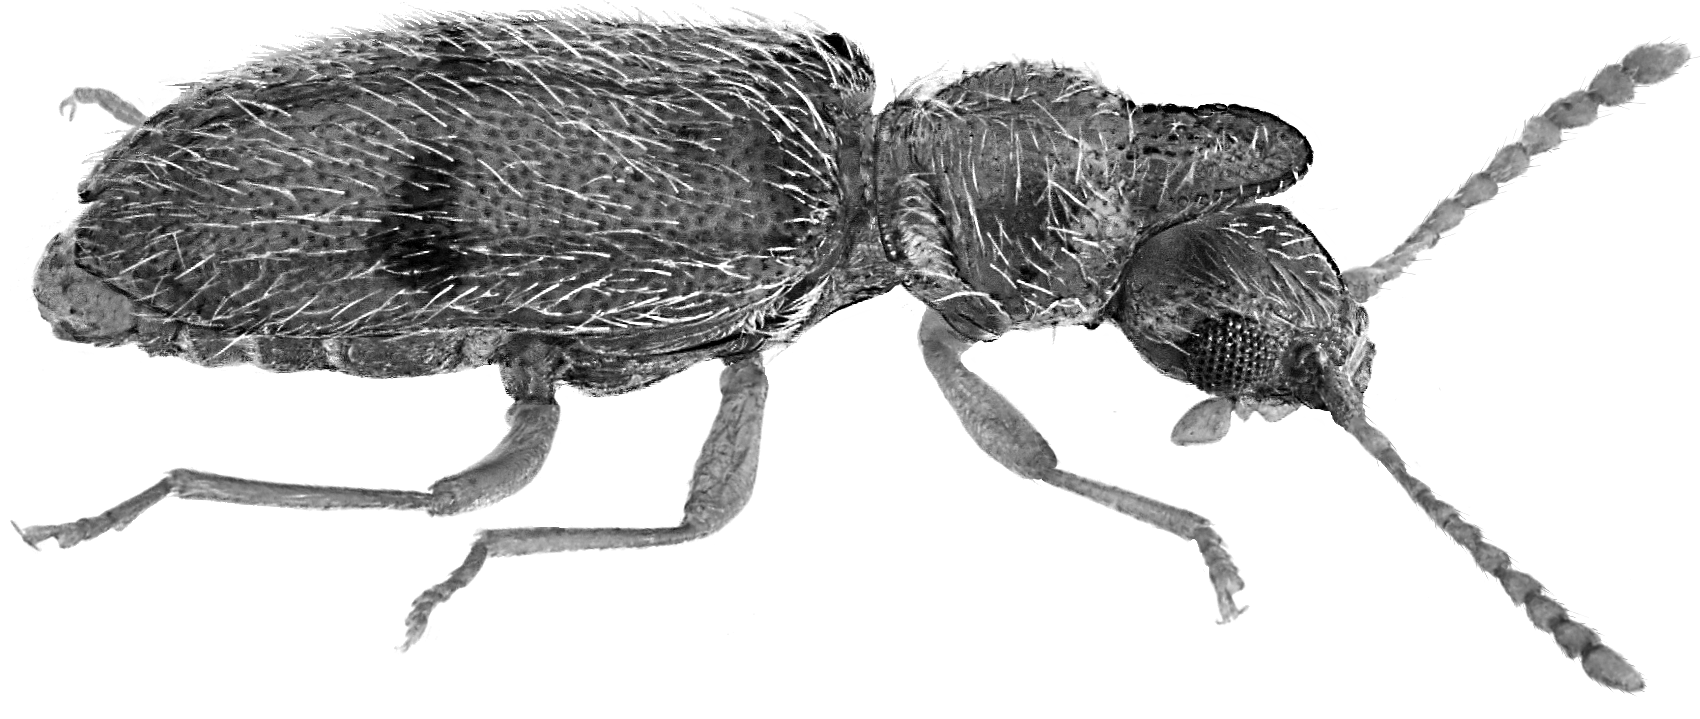
\includegraphics[width=\textwidth]{coleopterida/AnthicidHabitus}
  \caption{Anthicidae}
  \label{fig:anthicid}\end{subfigure}
    \caption{\textbf{(a)} Habitus (redrawn from photo (CC BY-SA 2.0) by Udo Schmidt \url{https://flic.kr/p/5uszAS}; \textbf{(b)} habitus (modified photo (CC BY-SA 2.0) by Udo Schmidt \url{https://flic.kr/p/qQRBXz})}\label{fig:anthmelo}
\end{figure}%need line drawing or black and white

\subsubsection{Anthicidae (ant-like flower beetles)}\index{Anthicidae}
\noindent{}\textit{Diagnostic characters:} Head as wide as pronotum, with ``neck'' (\textit{i.e.}, constriction behind eyes); pronotum widest near front, narrowed posteriorly, often with anterior pronotal horn; elytra often setose; antennae threadlike to weakly clubbed; Some have short elytra- tell apart from Staphylinidae by the hind coxae with a posterior face.\vspace{3mm}

\noindent{}\textit{Natural history:} Larvae and adults feed on a diverse array of foods. About 3,000 species have been described worldwide.

\subsubsection{Tenebrionidae (darkling beetles)}\index{Tenebrionidae}
\noindent{}\textit{Diagnostic characters:} Tarsi 5-5-4 (most beetles have 5-5-5); trochantin concealed or absent; eyes usually notched by frontal ridge (emarginate); antennae arising from under ridge on frons so that insertion can't be seen dorsally; antennae threadlike, bead-like to very weakly clubbed; 3 anteriormost sternites connate (fused); extremely variable in form.\vspace{3mm}

\noindent{}\textit{Natural history:} A diverse family, with at least 20,000 described species. Their diets vary, but most species seem to be fungivores and/or saprophages. These beetles are frequently found in xeric environments. \textit{Tenebrio molitor} Linnaeus, 1758, an important model for genetic research, is a tenebrionid.


\begin{figure}[ht!]
  \centering
    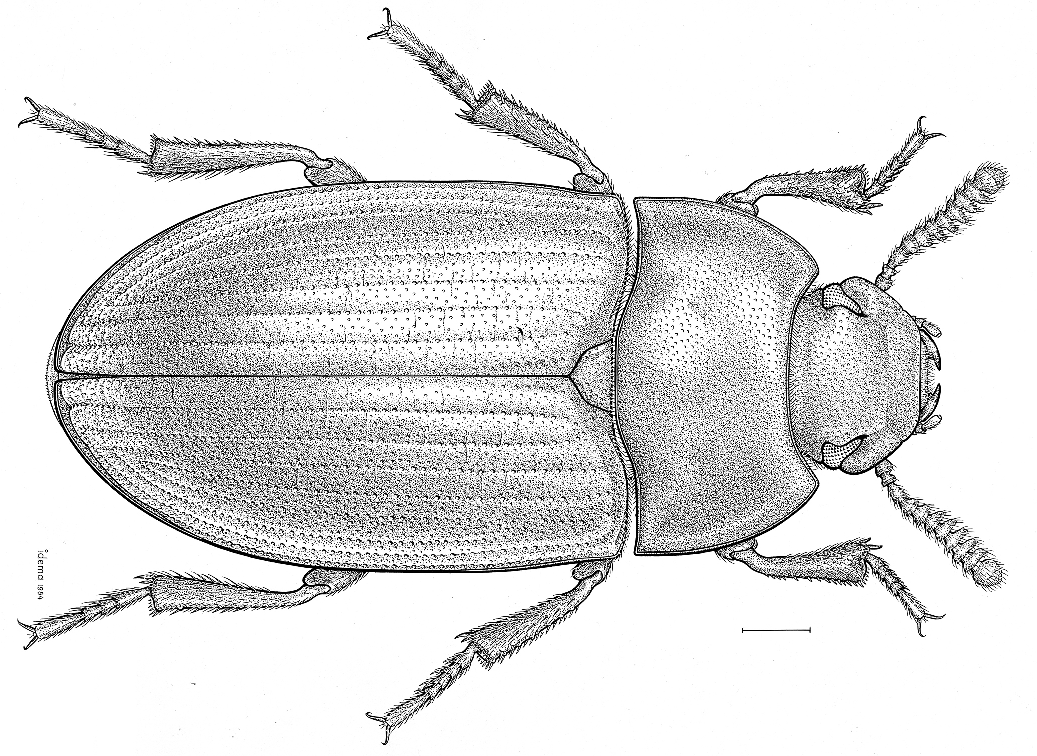
\includegraphics[width=0.55\textwidth]{coleopterida/TenebrionidHabitus}
  \caption{Tenebrionidae habitus (illustration (CC BY 4.0) by Roelof (Ralf) Idema; source: \url{https://doi.org/10.3897/zookeys.728.20602.figure15})}
  \label{fig:tenebrionids}
\end{figure}

\subsubsection{Coccinellidae (ladybird beetles)}\index{Coccinellidae}
\noindent{}\textit{Diagnostic characters:} Tarsi 4-4-4, often apparently 3-3-3 (\textit{i.e.}, pseudotrimerous; antennae short, with weak 3--6-merous club; pronotum wide but often concealing head dorsally; 2 anteriormost sternites connate (fused); first abdominal segment with lines leading from coxa.\vspace{3mm}

\noindent{}\textit{Natural history:} These beetles are primarily predators of other insects, especially soft-bodied ones, like aphids. Like meloids, these beetles are usually capable of reflex-bleeding as a defense; their hemolymph is toxic. About 6,000 species have been described.

\begin{figure}[ht!]
  \centering
\begin{subfigure}[ht!]{0.42\textwidth}
    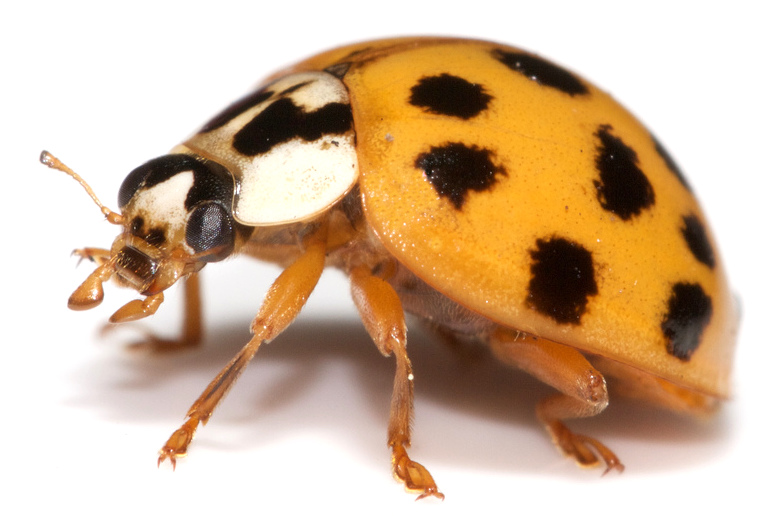
\includegraphics[width=\textwidth]{coleopterida/CoccinellidLateral}
  \caption{}%need line drawing or black and white
  \label{fig:coccinellid1}
\end{subfigure}
    \qquad
\begin{subfigure}[ht!]{0.39\textwidth}
    \reflectbox{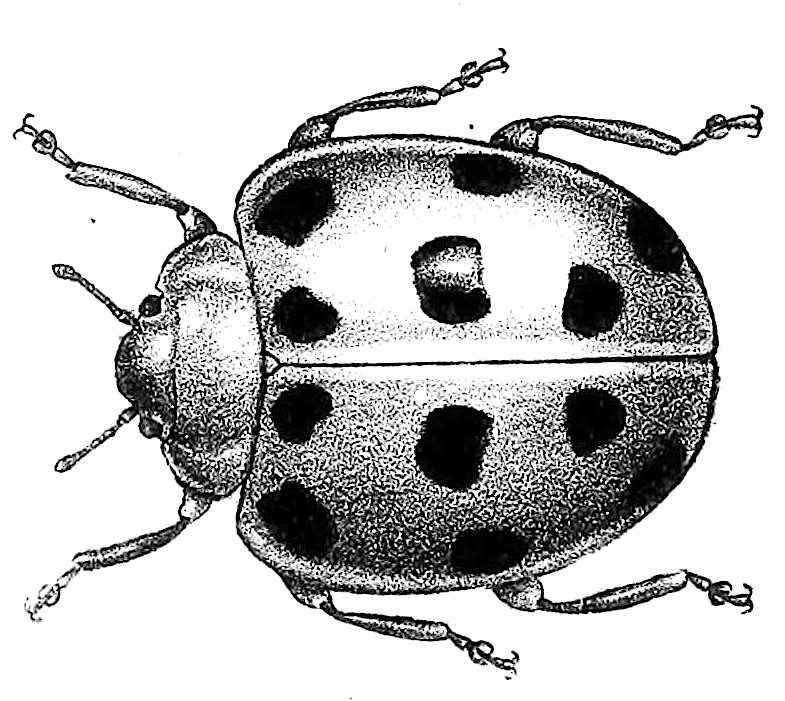
\includegraphics[width=\textwidth]{coleopterida/CoccinellidHabitus}}
  \caption{}
  \label{fig:coccinellid2}
\end{subfigure}
    \caption{Coccinellidae. \textbf{(a)} Lateral habitus, photo (CC BY 2.0) by Brian Gatwicke \url{https://flic.kr/p/HUpi9W}; \textbf{(b)} dorsal habitus \citep[modified from][Plate 10, Fig. 6]{bhlitem112390}}\label{fig:coccinellids}
\end{figure}

\noindent{}The remaining families are classified in a taxon called \textbf{Phytophaga}, and the vast majority of these species feed on plants. All species are 5-5-5 but look 4-4-4. \index{Phytophaga}

\subsubsection{Cerambycidae (longhorn, longicorn beetles)}\index{Cerambycidae}
\noindent{}\textit{Diagnostic characters:} Tarsi 5-5-5, pseudotetramerous; femora often enlarged, palpi often very short and immovable; antennae long, not clubbed, usually longer than half the body and often longer than body, capable of reflexing back over body; eyes usually notched, antennal insertion often protruding and arising from notch; tibiae always with 2 large apical spurs; body 3--75 mm long.\vspace{3mm}

\noindent{}\textit{Natural history:} Extraordinarily diverse family, with \textgreater30,000 known species. Larvae usually live inside and feed on dead or dying wood. Adults can be found foraging on pollen, nectar, fungi, and other foods. This family includes many significant forest pests (\textit{e.g.}, the Asian Long-horned Beetle, \textit{Anoplophora glabripennis} (Motschulsky, 1853)).

\begin{figure}[ht!]%https://flic.kr/p/Dosipm      https://www.biodiversitylibrary.org/page/58020956   https://commons.wikimedia.org/wiki/Category:Arcana_Naturae_(Thomson)#/media/File:Arcana_natur%C3%A6_(VOL._I._Pl._VI)_BHL36104298.jpg    https://commons.wikimedia.org/wiki/Category:Fauna_of_British_India_including_Ceylon_and_Burma_(Coleoptera)#/media/File:Xylotrechus_quadripes_FBI.jpg
  \centering
\begin{subfigure}[ht!]{0.44\textwidth}
    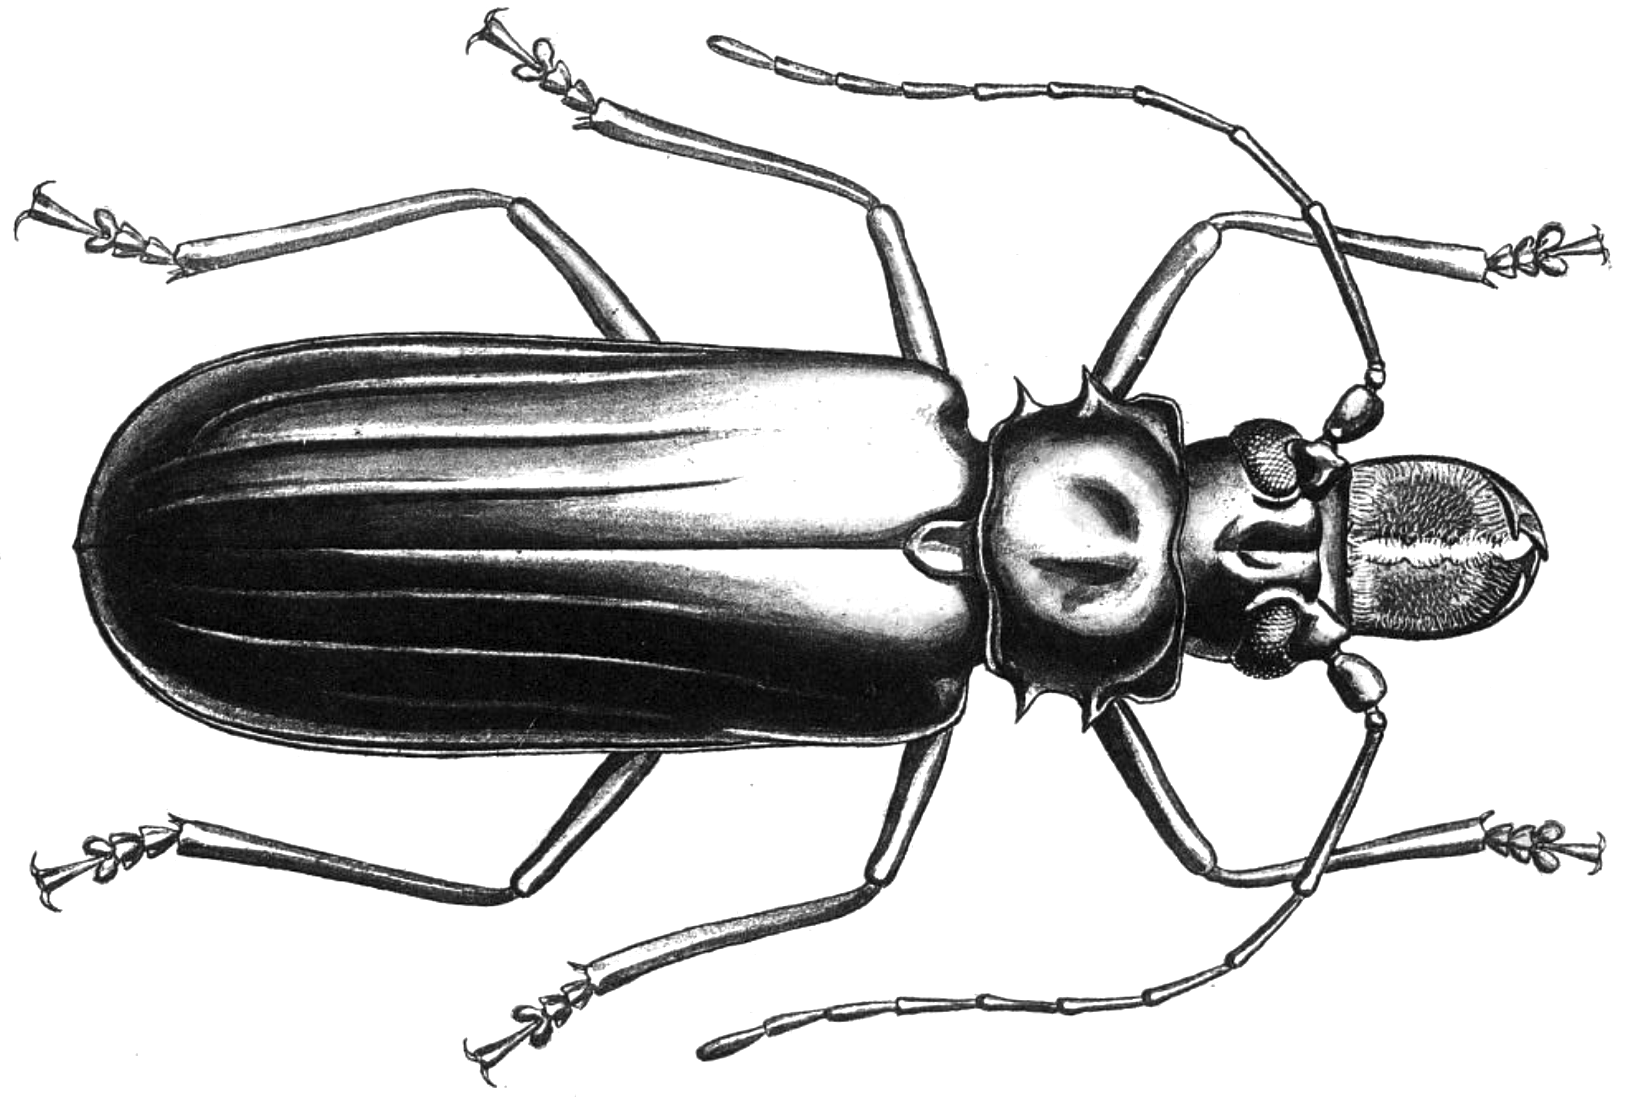
\includegraphics[width=\textwidth]{coleopterida/Cerambycid1}
  \caption{}
  \label{fig:cerambycid1}
\end{subfigure}
\hfill
\begin{subfigure}[ht!]{0.47\textwidth}
    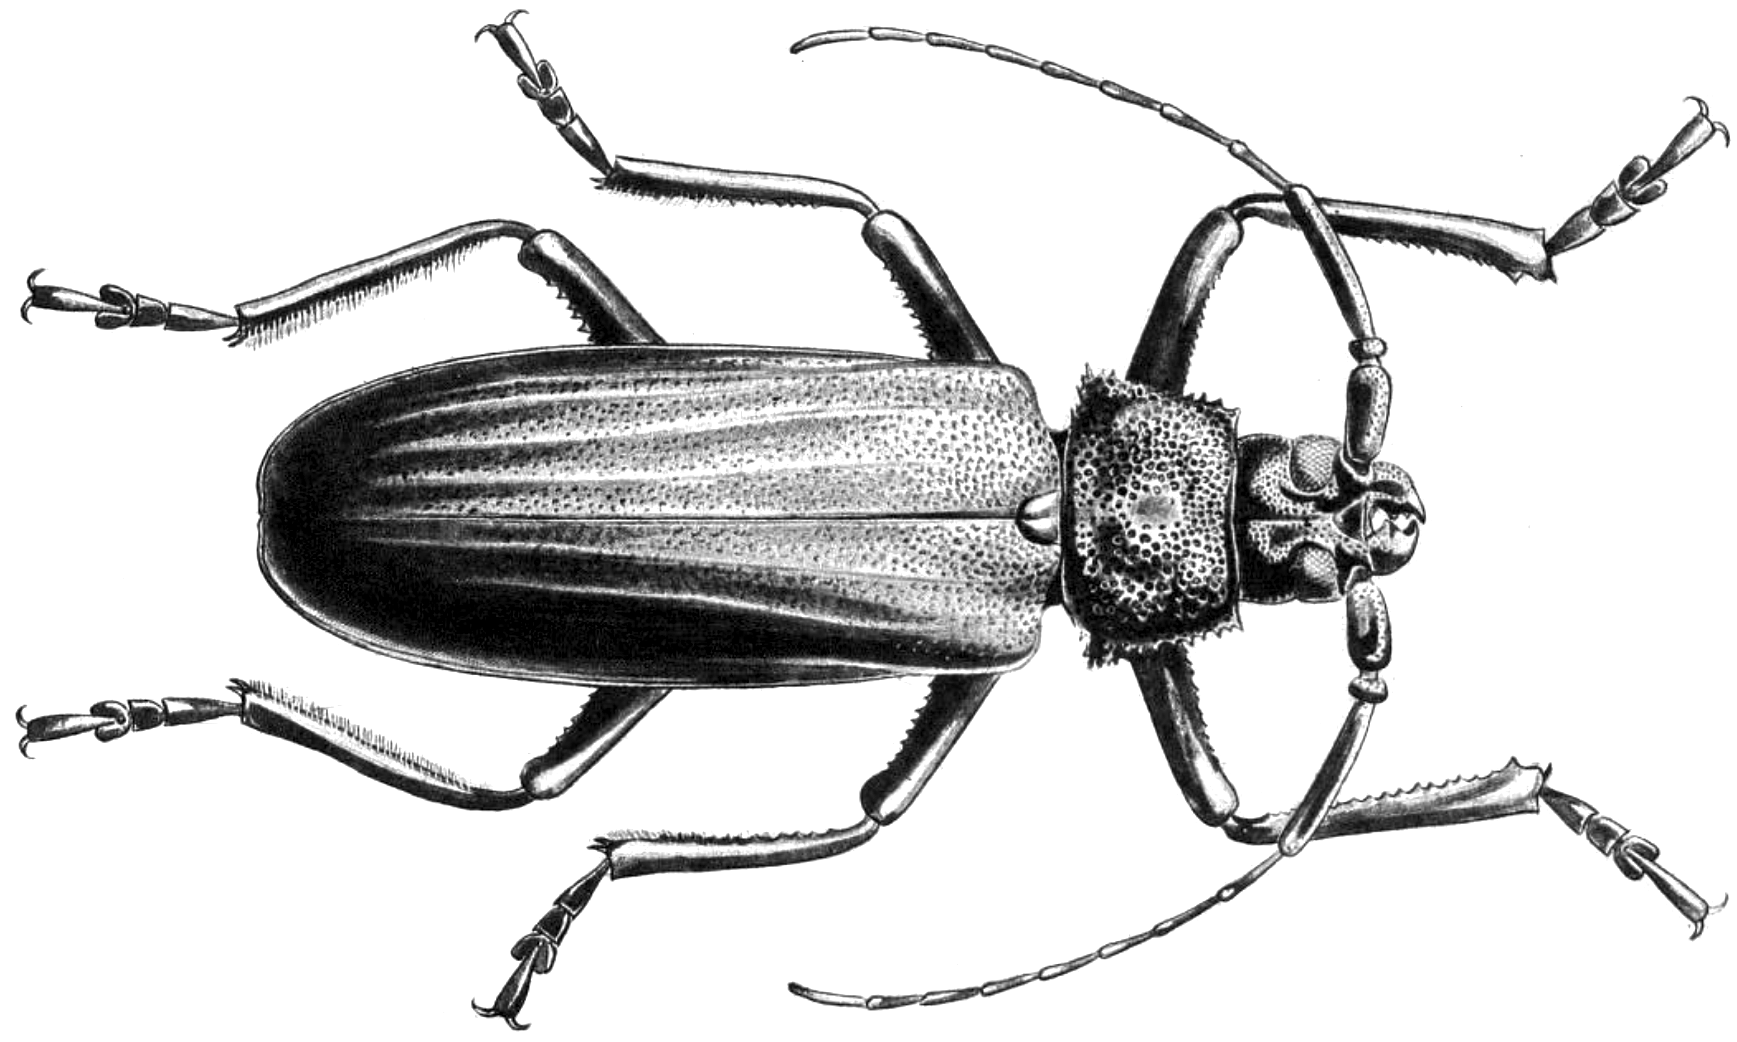
\includegraphics[width=\textwidth]{coleopterida/Cerambycid3}
  \caption{}
  \label{fig:cerambycid3}
\end{subfigure}
    \caption{Cerambycidae \citep[modified from][Plates II-III, Fig. 7]{bhlitem103087}}\label{fig:cerambycids}
\end{figure}

\subsubsection{Chrysomelidae (leaf, bean beetles)}\index{Chrysomelidae}
\noindent{}\textit{Diagnostic characters:} Tarsi 5-5-5, pseudotetramerous; femora often enlarged, palpi often very short and immovable; antennae shorter than half the body, not clubbed, if longer then not arising not prominent notch in eye ; usually at least one tibia with less than 2 apical spurs; can be very difficult to tell apart from Cerambycidae (but antennae are not arising from frontal tubercles); subfamilies often distinctive; usually small, body rarely \textgreater12 mm long.\vspace{3mm}

\noindent{}\textit{Natural history:} Diversely phytophagous beetles, with species foraging on just about every part of the plant imaginable---leaves, seeds, stems, roots, \textit{etc}. At least 37,000 species are known, and they are phenotypically quite diverse.

\begin{figure}[ht!]
  \centering
    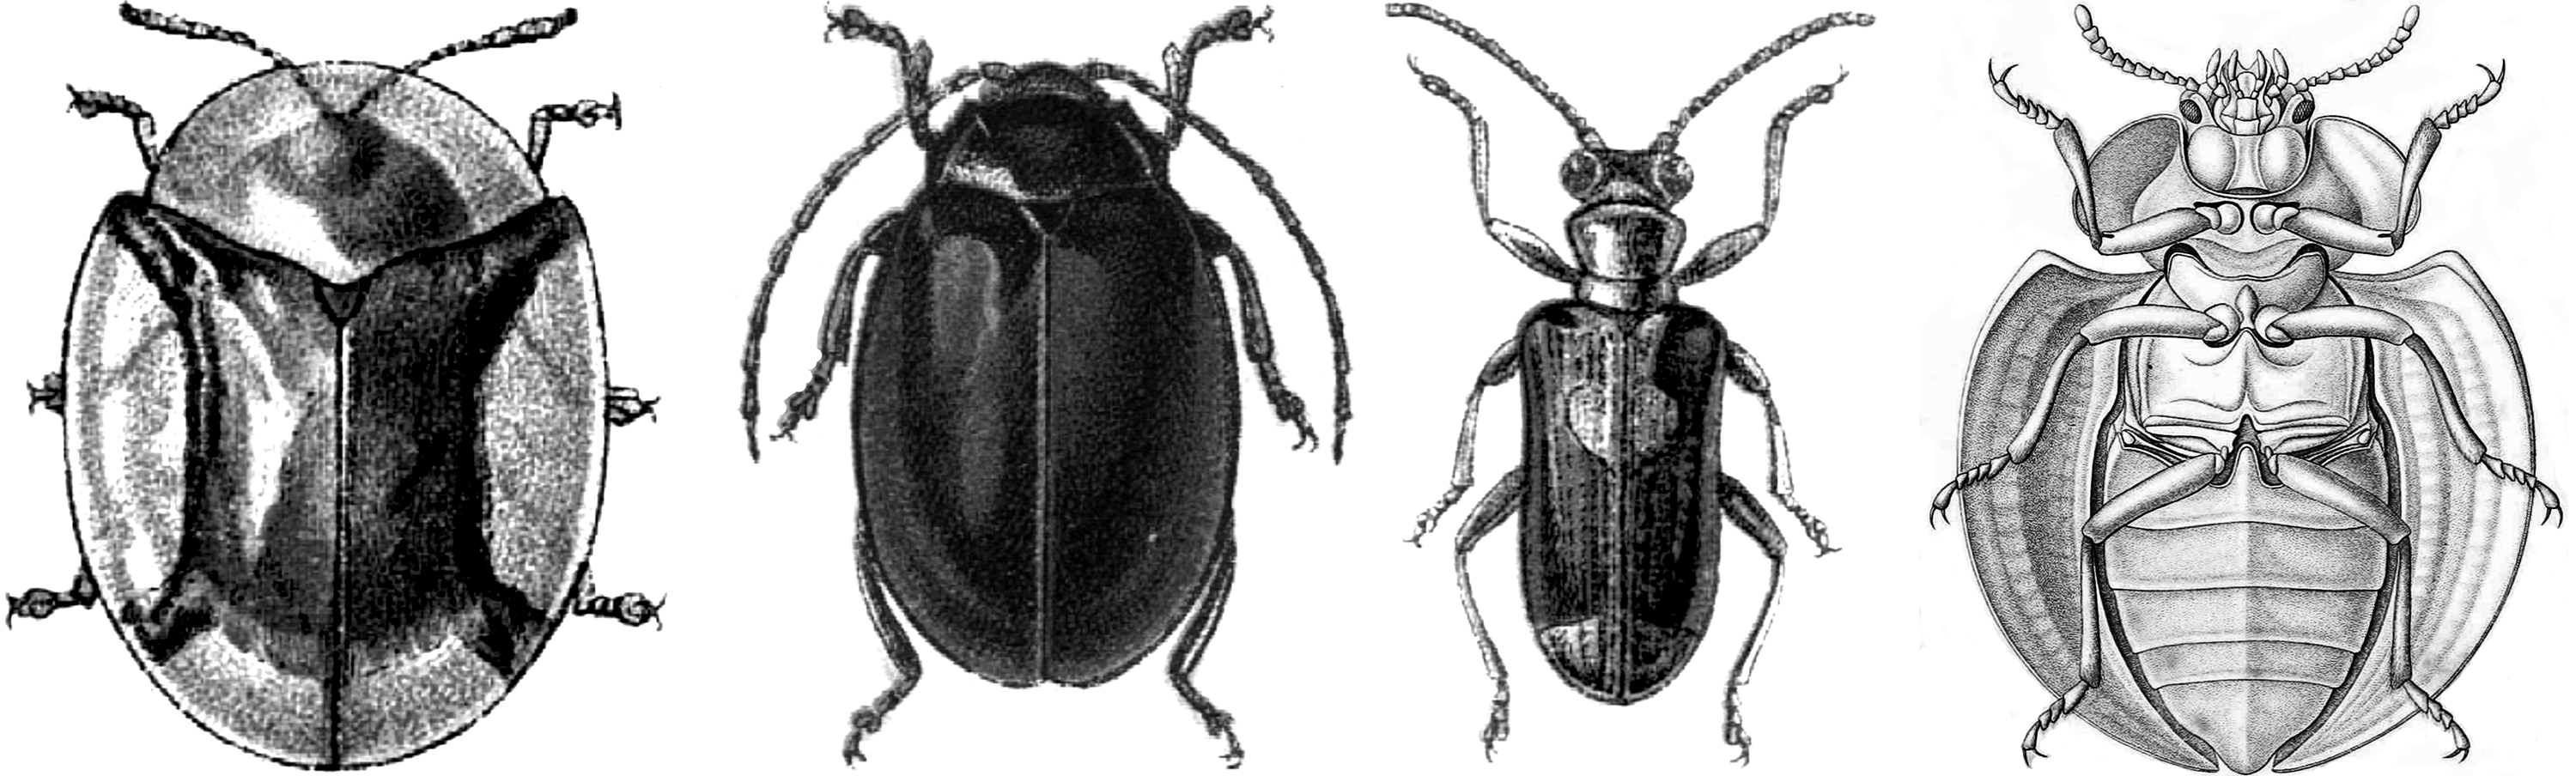
\includegraphics[width=0.98\textwidth]{coleopterida/chrysomelids}
  \caption{Chrysomelidae dorsal habitus \cite[redrawn from][Plate 61, Figs. 18, 24, 33]{bhlitem240513beetles}; ventral habitus \citep[modified from][Plate 1, Fig. 1]{bhlitem35775}}
  \label{fig:chrysomelids}
\end{figure}

\subsubsection{Curculionidae (weevils, bark beetles)}\index{Curculionidae}
\noindent{}\textit{Diagnostic characters:} Tarsi 5-5-5, pseudotetramerous; femora often enlarged; snout usually well developed, flat or slender, mandibles often tiny, palpi very short and immovable; antennae elbowed, with compact 3--4-merous club, usually arising on snout. This lineage includes numerous important pests.\vspace{3mm}

\noindent{}\textit{Natural history:} Easily the most diverse family of insects (and likely of anything living), with \textgreater80,000(!) described species. They are diversely phytophagous, although many species (ambrosia beetles; formerly Platypodidae and Scolytidae) cultivate fungi in galleries inside trees. Several other families of weevil-like beetles in this region are not covered in this manual; be sure to key your specimens!

\begin{figure}[ht!]
  \centering
    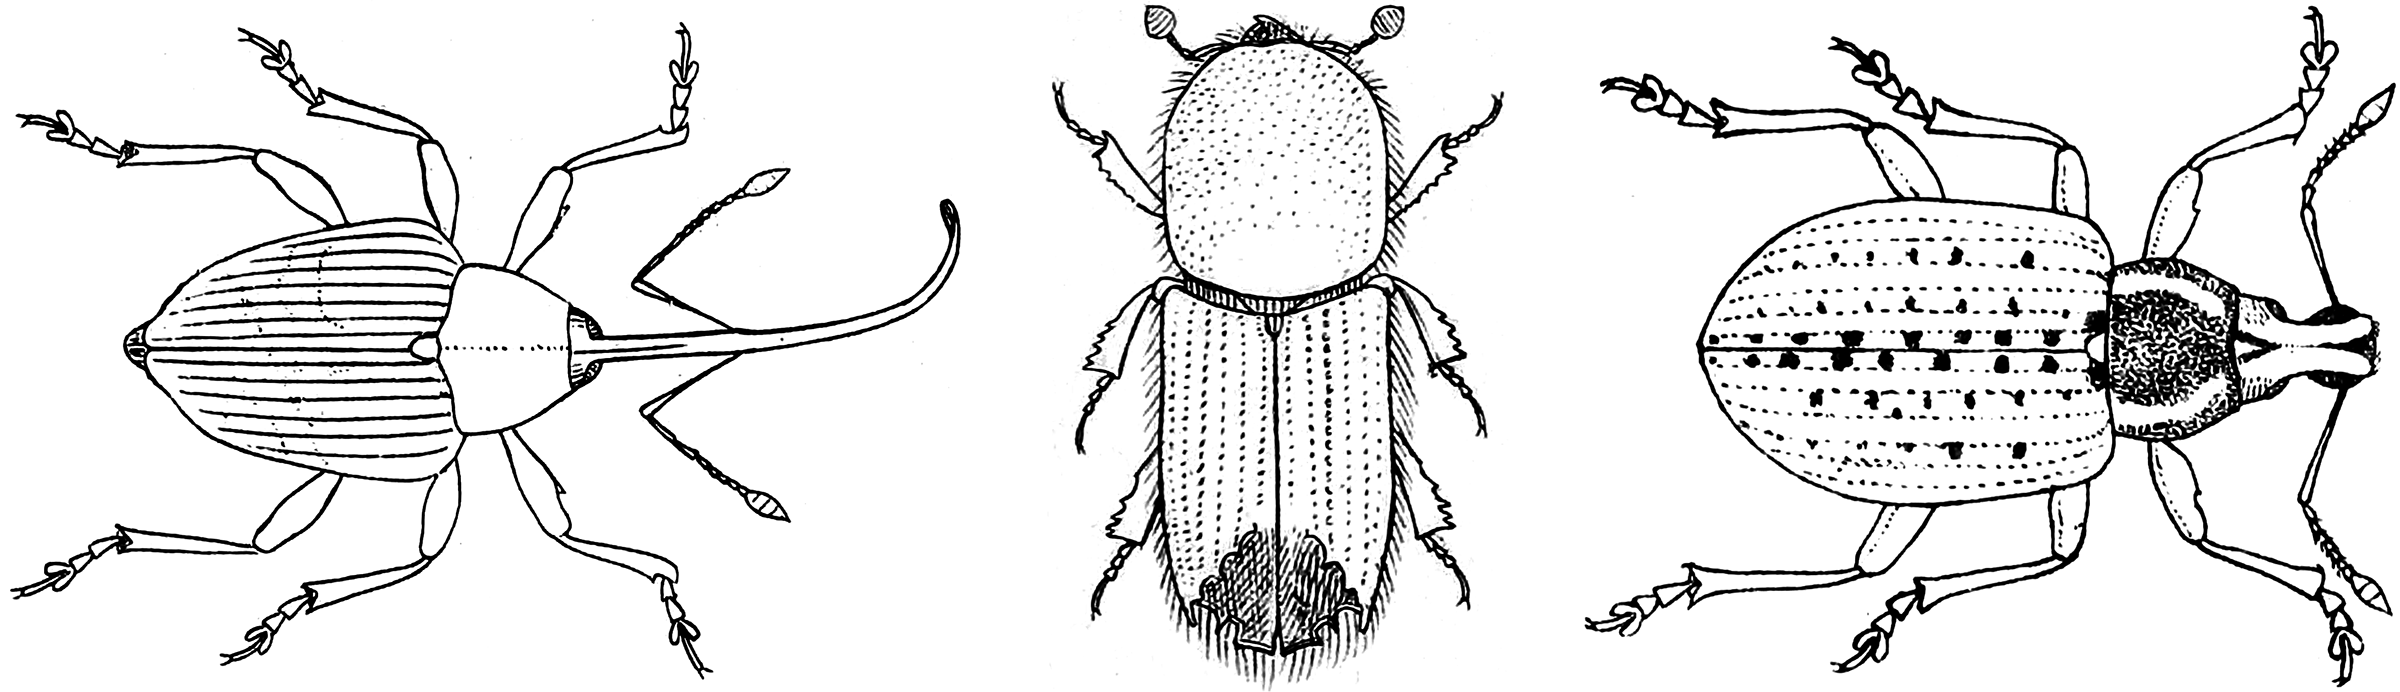
\includegraphics[width=0.98\textwidth]{coleopterida/curculionids}
  \caption{Curculionidae \cite[redrawn from][Plate 67, Fig. 8; Plate 73, Fig. 7; Plate 71, Fig. 6]{bhlitem37317beetles}}
  \label{fig:curculionids}
\end{figure}

\FloatBarrier
\section{Strepsiptera (twisted-wing parasites)}\index{Strepsiptera}
Coleoptera's sister, \textbf{Strepsiptera}, includes relatively few species, all of which are parasitic on other insects. We will learn them only at the ordinal level.
\begin{itemize}
\item fore wing reduced to short club-like structures (like hind wing halteres of Diptera)
\item hind wing large and fan-like, with few veins
\item antennae 4--7-segmented, usually branched
\item eyes bulging or on stalks
\item females usually do not leave the host and look more or less like a legless engorged tick embedded between the abdominal segments of their host
\item minuscule triungulin first instar larvae (distinctive larval phenotype with 3 tarsal claws)
\end{itemize}

\begin{figure}[ht!]
  \centering
\begin{subfigure}[ht!]{0.5\textwidth}
    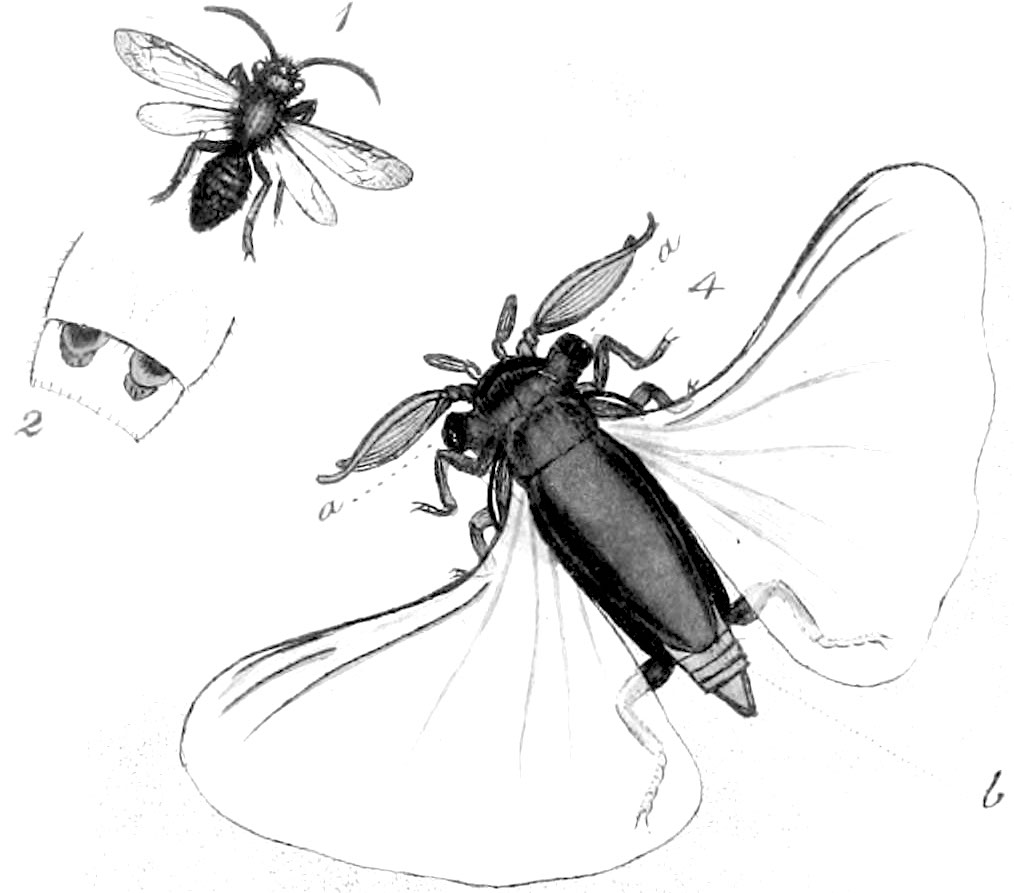
\includegraphics[width=\textwidth]{coleopterida/Strepsiptera1}
  \caption{}
  \label{fig:strep1}
\end{subfigure}
    \hfill
\begin{subfigure}[ht!]{0.45\textwidth}
    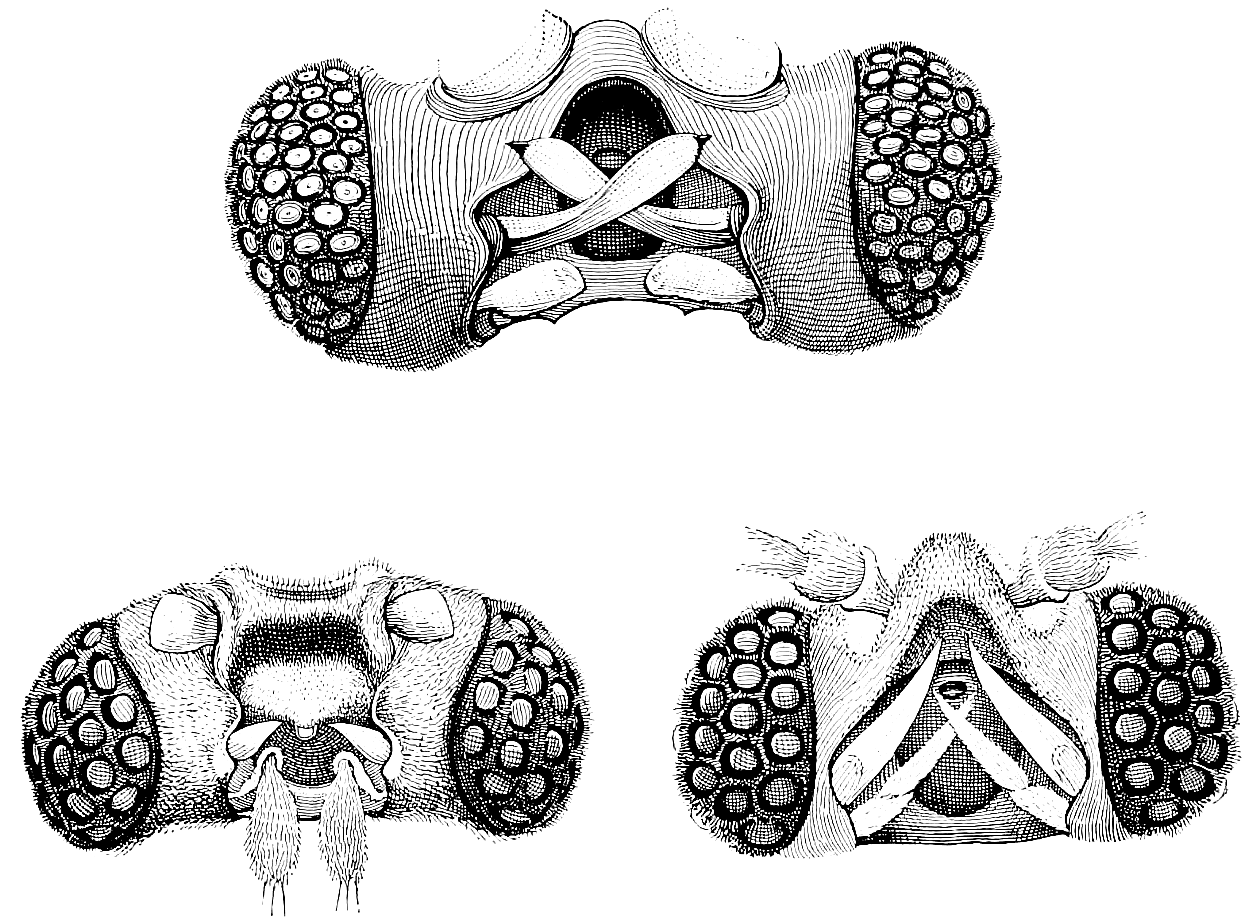
\includegraphics[width=\textwidth]{coleopterida/strepsipteraHead}
  \caption{}
  \label{fig:strep2}
\end{subfigure}
    \caption{Strepsiptera. \textbf{(a)} Inside host (upper left); male (lower right) \citep[Plate 45 in][]{bhl91785}; \textbf{(b)} heads, with distinctive eyes \citep[modified from][Plate I, Figs. 4--6]{bhlitem53053stylopidae}}\label{fig:strepsipterans}
\end{figure}

\section*{Test yourself}
Before moving on to the next unit make sure you are comfortable with the following concepts. Could you write a couple sentences that explain each term? Can you provide examples?\vspace{3mm}

\noindent{}What selective advantages do elytra confer to these insects? What factors \textit{besides} the presence of elytra might explain the extraordinary diversity of beetles?\vspace{3mm}

\noindent{}What adaptations do we see in Adephaga, and how do they contribute to the diversity of the lineage and its classification?\vspace{3mm}

\noindent{}Would you describe strepsipterans as parasites or parasitoids? Why?\vspace{3mm}

\noindent{}Familiarize yourself with the following taxon names, which refer to organisms you are likely to encounter in the northeastern USA and/or which are phylogenetically relevant. Can you describe how these arthropods live (natural history) and roughly how diverse they are? Do you know how they're related to one another? If you had to choose a family to study from the taxa below which one would it be and why?
\begin{enumerate} 
\item Archostemata
\item Adephaga
\item Coleoptera  
\item Phytophaga
\item Polyphaga
\item Strepsiptera
\end{enumerate}

\clearpage
\thispagestyle{empty}